\RequirePackage{lineno}
\documentclass[12pt,a4paper]{article}
\usepackage[T1]{fontenc}
\usepackage{graphicx}
\usepackage{hyperref}
\usepackage{caption}
\usepackage{mathptmx}
\usepackage[absolute,overlay]{textpos}
\usepackage{fancybox}
\usepackage{multirow}
\usepackage[dvipsnames]{xcolor}
\usepackage{amsmath, amsthm, amssymb,amsfonts}
\usepackage{float}
\usepackage{fullpage}
\usepackage{units}
\usepackage{xspace}
\usepackage{caption}
\usepackage{subcaption}

%%% Code to enter C++ code
\usepackage{listings}
\linenumbers % Include line numbers
\lstset{language=C++,
        basicstyle=\ttfamily,
        keywordstyle=\color{blue}\ttfamily,
        stringstyle=\color{red}\ttfamily,
        commentstyle=\color{green}\ttfamily,
        morecomment=[l][\color{magenta}]{\#}
}

\usepackage{hyperref}
\hypersetup{
    colorlinks,
    citecolor=blue!90!black,
    filecolor=black,
    linkcolor=blue!50!black,
    urlcolor=blue!50!black
}

\author{Robert Kralik\\\small{University of Sussex}}
\title{NOvA Test Beam detector calibration\\ \vspace*{5mm}
\Large{Technical Note}}
\date{\today}

\begin{document}
\maketitle
\begin{abstract}
What is this about and what will I describe in here
\end{abstract}
\tableofcontents
\newpage

\section{Introduction}
TO DO:
\begin{itemize}
\item Divide the motivation to abstract (why do we care about test beam calibration, what did we do and how did we do it. What are the results)
\item and introduction (brief history of test beam calibration, maybe a bit more detail into why is test beam calibration imporant)
\end{itemize}

Why is Test Beam?
"The idea, as with any test beam experiment, is to expose a detector to a beam of very well-characterized particles, so that we can improve our understanding our how the detector responds to such particles. We make use of upstream detectors to collect data on the beam particles before they interact in the NOvA detector. For example, we will be able to see what a 1 GeV proton actually looks like in our detector, without having to simulate it, and we can test how well we would have reconstructed the energy using our existing techniques. We may find we are able to make improvements to our tools to better match what we see in the detector with how we reconstruct it. Or we may find we already do a pretty good job. Either way, with a full cross-comparison like this, we can be more confident in our analysis of the data and reduce the level of uncertainty we consider are associated with the relevant measured quantities. Ultimately, the aim will be to reduce the level of uncertainty on the neutrino oscillation analyses and to make even better, more accurate measurements of the Standard Model."%[https://cdcvs.fnal.gov/redmine/projects/novatestbeam/wiki/Introduction_to_Test_Beam_for_Analyzers]
Why is Test Beam calibration done:
\begin{itemize}
\item To be able to directly compare TB to the standard detectors
\item To be able to verify our calibration procedures using TB data
\item To study the particle response as a function of energy 
\item To determine an energy resolution
\item To compare currently used energy scales to data and understand if we can use TB data for absolute energy scale in all NOvA detectors
\end{itemize}

%Only considering improvement in the calibration systematic uncertainty, the NOvA Test Beam program can reduce the overal systematic uncertainty for the main NOvA measurements by about 10\% [docdb:33012] (talk also contains a list of other talks on impact of TB in different NOvA areas). 
For DeltaM2: By increasing exposure, total syst. error decreases by (+) 18.5% (-) 25%; By increasing exposure and reducing calib systs., total syst. error decreases by: (+) 26% (-) 32%; Difference between the above (reducing calib systs. with large exposure): (+) 9.6% (-) 9.4%.
For sin2Th23: Difference by reducing calib syst.: (+) 10.8% (-) 9.4%.
Statement: “The NOvA Test Beam will improve the total systema6c error on the final measurement of the oscilla6on parameters Dm232 and sin2Th23 by 10% from reduc6on of calibra6on systema6cs alone. Further, NOvA analyses will benefit from the detailed understanding of detector response to hadronic, electromagne6c, and muon energy provided by the Test Beam, which will be essen6al to solidify understanding of systema6cs, uncover poten6ally new uncertain6es, tune the simula6on modeling, and improve reconstruc6on and PID algorithms.”
Potential Test Beam impacts: Check modeling of hadronic interacOons in detector (check GEANT systemaOcs), Using Test Beam data as “single-parOcle MC” to train CVN prong-like algorithms, GeneraOve Adversarial Networks for MC improvements using Test Beam data, Check ND calibraOon procedure to try and understand causes of 3-5% discrepancy between data and MC for muons and protons  (Birks suppression measurement), Data/MC comparisons of observed and clustered visible energy to improve dead material correcOons and energy esOmators, Acquire beier understanding of gain and photon transport, aienuaOon, Cherenkov light modeling, [DifferenOal] charged pion and proton cross secOon measurements would be extremely useful!, CalibraOng with test beam muons vs. cosmic muons (differences between horizontal vs. verOcal muons? - possibly shed “light” on the calib shape uncertainty), Study path length inside cell, take beam data with non-orthogonal incidence, Cross-check pi0 invariant mass reconstrucOon and Michel tagging efficiency/spectra, Use neutron source to study modeling of neutron capture (I don't think this was done in the end...), Playing with different GEANT physics lists to boost our confidence in the MC (pions? neutrons?)

%[docdb:25074 - The NOvA Test Beam program paper for DOE] Improvements which enable these physics milestones include reduction of the experiment systematic uncertainties of which many are related to the energy calibration of the detector... Achieving 3sigma CP sensitivity requires all of the above factors; a failure to reduce systematic uncertainties puts this opportunity out of reach. The NOvA test beam effort will provide tagged electron, muon, pion, and proton beams which will enable a detailed understanding of the detector’s muon energy scale, electromagnetic and hadronic response in addition to providing real data for the detailed study of particle identification techniques. Muon energy scale, hadron energy scale, and scintillation model uncertainties combine to contribute 90% of the total systematic error budget for sin2 th23 and would directly benefit from test beam data. A reduction by half would keep them comparable to the final statistical precision of the experiment. Recent oscillation analyses have had to account for large differences between data and simulation in the hadronic energy recorded in the near detector through changes to the detector response and neutrino cross-sections. Our calibration systematic uncertainty is dominated by a 5% difference between the calibrated detector response for muons and protons. Energy calibration and detector response contribute 50% of the total systematic error in electron neutrino appearance. Improved understanding of the detector response will help factor the product (flux × cross-section × detector response) improving future cross-section measurements. The most important impact on the electron-neutrino appearance measurement will likely be the opportunity to verify and improve particle identification algorithms.

%[docdb:15750 - NOvA Test Beam task force report]: The test beam program was included in the NOvA proposal [1] and was considered as an essential part of the experiment since its inception. The main tangible result of these initial plans and later discussions was a production of special small extrusion modules, made at the end of the modules production stage, as possible components of a future test beam detector. In fact, this production followed and was based on initial simulations of a possible test beam experiment [5]. rimary goals are oriented toward measurements of detector response to different particles with a range of momenta most relevant to NOvA beam physics studies, establishing of the absolute and relative energy scale of both NOvA detectors, and validating detailed and fast detector simulations code. [List all possible desired studies with Test Beam copied below] Two 31-layer 2 × 2 blocks, with approximate dimensions of 2.6 × 2.6 × 4 m3 were produced at the Minnesota factory before its shutdown (as a comparison, the 3 × 3 NOvA ND has 6 × 32 layers). In addition, 96 1 × 1 layers, with approximate total dimensions of 1.3 × 1.3 × 6.2 m3 were produced. Both 2 × 2 blocks and all the 1 × 1 layers were leak-tested. The 2 × 2 blocks are currently stored at the MINOS surface building, while the 1 × 1 layers are stored at the CDF building(?). The proposed detector to be deployed for the test beam run consists of the two 2 × 2 blocks. The NDOS decommissioning yielded 25000 gallons of scintillator. Since storage available is limited to 12000 gallons, it was decided to blend most of the 5000 gallons of existing ND/FD scintillator with the NDOS scintillator. 200 gallons of ND/FD scintillator, which has a slightly higher photon yield, are reserved for special studies. We also plan to reuse the NDOS secondary containment tub to provide oil+scintillator containment in case the test beam detector undergoes a catastrophic structural failure. Based on MINERvA’s experience, it is anticipated that two months of data taking would provide the necessary samples to carry out the test beam objectives.
\begin{itemize}
\item Hadronic response and comparison with MC modeling
\begin{itemize}
\item response as a function of energy
\item establishing of an absolute energy scale
\item determination of energy resolution
\item studies of topological features and resolution
\begin{itemize}
\item pion tracking and showers
\item proton tracking and showers
\end{itemize}
\item studies of timing features and resolution
\end{itemize}
\item Electromagnetic response and comparison with MC modeling
\begin{itemize}
\item response as a function of energy
\item establishing of an absolute energy scale
\item determination of energy resolution
\item studies of topological features and resolution
\begin{itemize}
\item electron signatures
\item gamma signatures
\end{itemize}
\item studies of timing features and resolution
\item studies of $\pi^0$ from $\pi^-$ charge-exchange
\end{itemize}
\item Muon response and comparison with MC modeling
\begin{itemize}
\item comparison with detailed optical simulations
\item determination of energy resolution
\item studies of topological features and resolution
\item cross-talk studies
\item comparison to cosmic ray muons (requires a special trigger)
\item studies of the muon calibration protocol
\end{itemize}
\item Light yield and response studies as a function of particle type and detector configuration
\begin{itemize}
\item understanding the Cherenkov light contribution
\item vertical and horizontal responses and comparison with simulations
\item data with selected planes rotated by 45 and 90 degrees
\item slanted (angle) plane response (and subset of programs as above)
\item fiber attenuation studies
\item Birks’ constant studies
\end{itemize}
\item Near / Far readout comparison
\item Gather large libraries of particles at known energies and multiple angles of incidence to help develop a CNN prong ID. Also allows training of a particle-based CVN-like PID.
\end{itemize}

Also use information from:
\begin{itemize}
\item NOvA Test Beam Technical Statement of Work
\item NOvA Test Beam program (paper for DOE) [docdb:25074]
\item NOvA Test Beam task force report [docdb:15750]
\item Overview presentation of NOvA Test Beam [docdb:20495]
\item Test Beam support document [docdb:22172]
\item NOvA Test Beam program proceedings [docdb:55808]
\end{itemize}

Mike's proceedings from ICHEP 2020 \cite{WallbankProceedingsICHEP2020}.

%%%%%%%%%%%%%%%%%%%%%%%%%%%%%%%%%%%%%%%%%%%%%%%%%%%%%%%%%%%%%%%%%%%%%%%%%%%%%%%
%%%%%%%%%%%%%%%%%%%%%%%%%%%%%%%%%%%%%%%%%%%%%%%%%%%%%%%%%%%%%%%%%%%%%%%%%%%%%%%
%%%
%%%                       Test Beam detector description
%%%
%%%%%%%%%%%%%%%%%%%%%%%%%%%%%%%%%%%%%%%%%%%%%%%%%%%%%%%%%%%%%%%%%%%%%%%%%%%%%%%
\section{Overview of the Test Beam detector}
%What is Test Beam, how does the detector and beamline look like.
%Placed in MC7b together with a beamline instrumentation (no need to describe beamline).

The NOvA Test Beam detector is a scaled down version of the Near and Far Detectors shown on figure \ref{figTBDetector}. It is placed in the MC7b enclosure of the Fermilab Test Beam Facility in the path of the MCenter beamline with a variety of beamline detectors to measure and identify a range of particles with various momenta \cite{NOVA-doc-22172-v2}.

\begin{figure}[!ht]
\centering
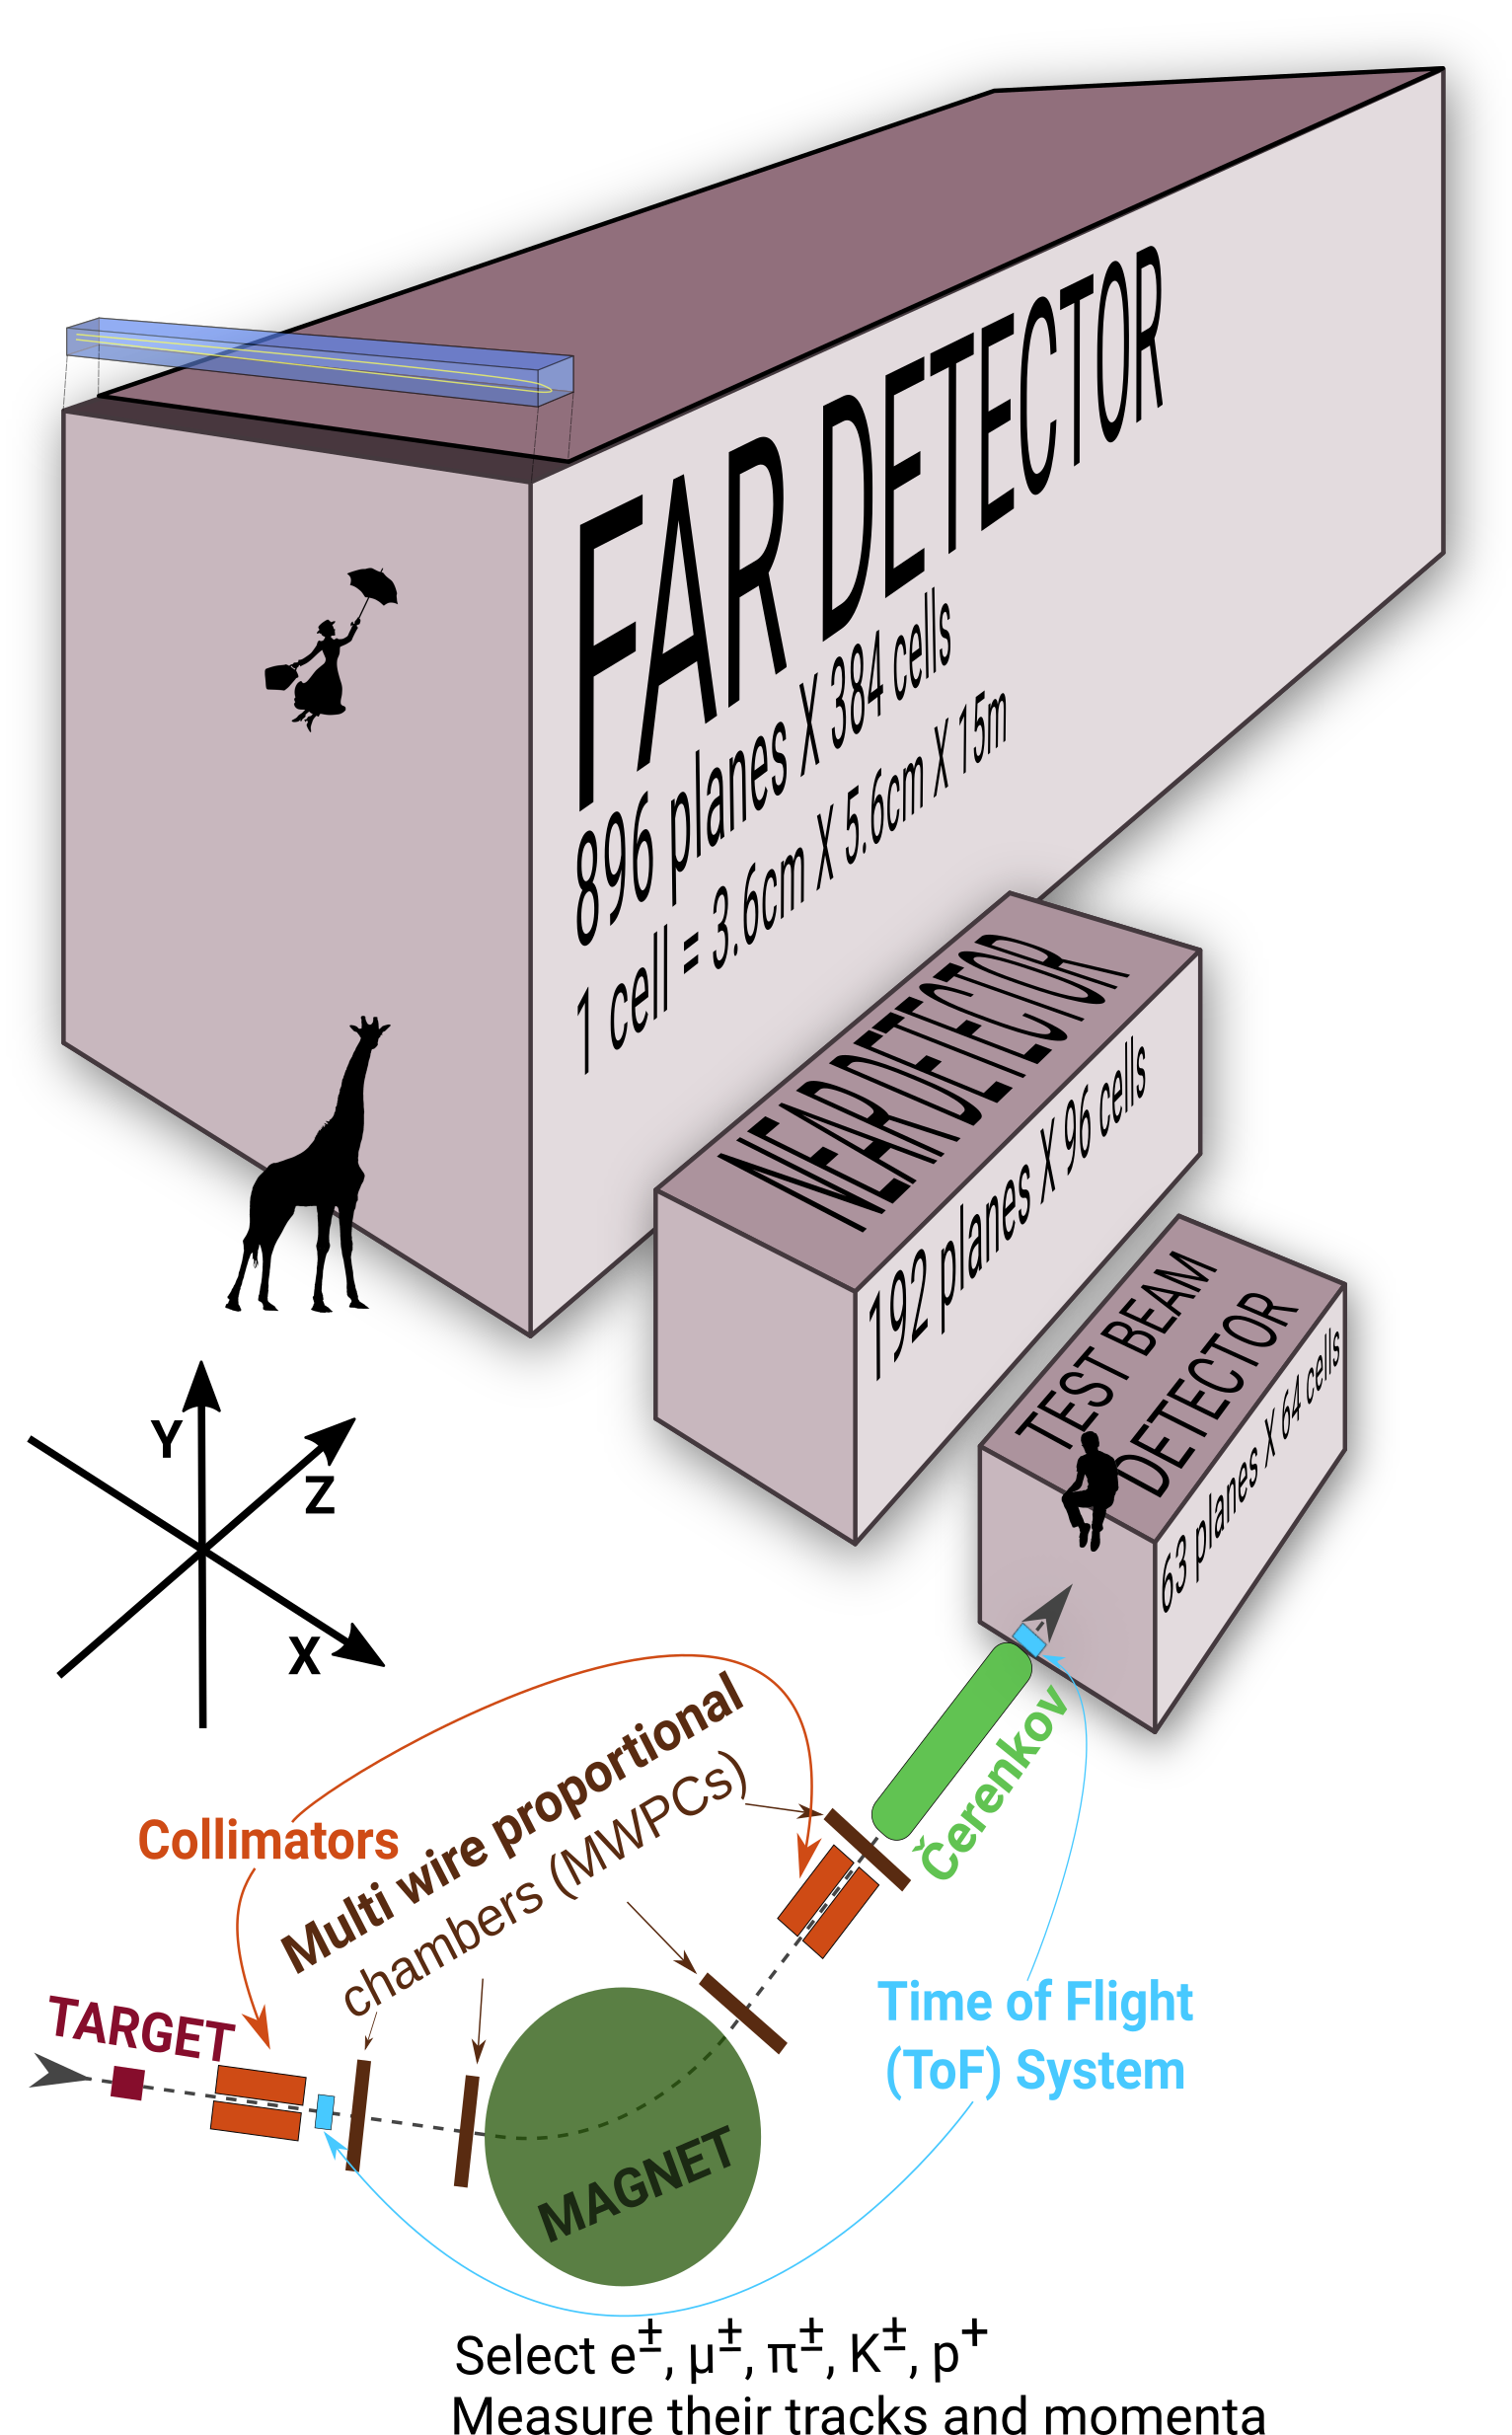
\includegraphics[width=.7\textwidth]{Plots/TestBeamDetectorWithArrows.png}
\caption{Comparison of Test Beam detector scale to the Near and Far NOvA detectors (and a man, giraffe, or Mary Poppins). Also shown are the Test Beam beamline detectors and components (not to scale), with arrows showing the direction of the beam. The three black arrows show the orientation fo the detector coordinate system.}
\label{figTBDetector}
\end{figure}

Maybe also mention the specific times Test Beam detector was operational.

Majority of the Test Beam detector and it's instrumentation is identical to the other NOvA detectors, but there are a few differences, including size, scintillator oil used, readout electronics, or environmental controls, that we're discussing in this section.

\subsubsection*{General parameters}
The NOvA Test Beam detector consists of two 31-plane blocks, each beginning and ending with a vertical plane, with an additional horizontal plane glued inbetween them to preserve the alternating arrangement \cite{NOVA-doc-29543}. Each plane consists of 2 modules side-by-side and each module is made up of 32 cells. Each cell has an inner (without the PVC) depth and width of $5.9\,\unit{cm}$ and $3.8\,\unit{cm}$ respectively, same as for the other NOvA detectors, and a length of $2.6\,\unit{m}$. This brigns the final dimensions of the Test Beam detector to 63 planes $\times$ 64 cells, or $2.6\times 2.6\times 4.1\,\unit{m^3}$.

The 63 planes are numbered from 0 to 62, with even numbers corresponding to vertical planes and odd numbers to horizontal planes. Cells are numbered 0 to 63, going from bottom to top for horizontal planes and left to right, when facing the front of the detector, for vertical planes.

The detector coordinate system is illustrated on figure \ref{figTBDetector}. It is centered with $\left(0,0,0\right)$ in the centre of the first plane \cite{NOVA-doc-58388}. The x axis runs left to right when facing the front of the detector, y axis bottom to top, and z axis goes along the beam direction from front to the back of the detector. The exact geometry of the Test Beam detector from several alignment surveys is saved in gdml files and used in our analyses \cite{NOVA-doc-57955}.

In the past we encountered an issue when aligning the Test Beam detector with the beamline measurements broke several assumptions within the Test Beam geometry \cite{NOVA-doc-58388}, which manifested as uncalibrated cells in the back of the detector \cite{NOVA-doc-57516-v2}. This was fixed by realigning both the detector and the beamline based on the last alignment survey and implemented in the production tag R23-04-05-testbeam-production.a and there after \cite{NOVA-doc-58388}.

%FD: maxPlane=900, maxCell=390. ND: maxPlane=220, maxCell=100. TB: maxPlane=63, maxCell=64

\subsubsection*{Scintillator}
The Test Beam detector is filled with (more than) three different versions of the NOvA scintillator, which differ mainly in the way they were stored since the filling of the near and far detectors. This is illustrated on figure \ref{figScintillators}.

\begin{figure}[!ht]
\centering
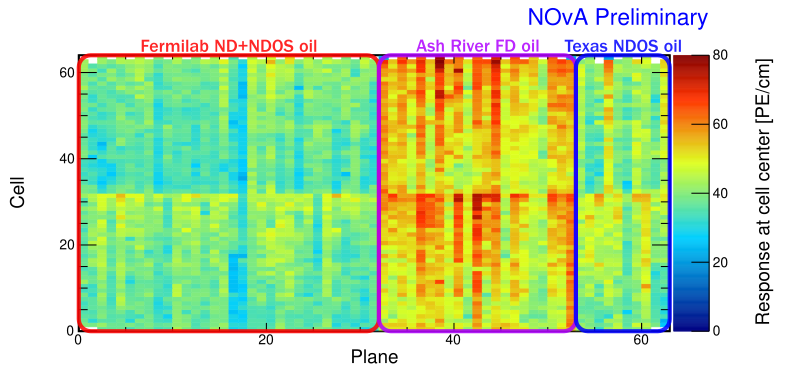
\includegraphics[width=\textwidth]{Plots/TestBeamScintillatorOils.png}
\caption{Uncorrected energy response in the centre of cells across the Test Beam detector showing a clear distinction between the different scintillator oils.}
\label{figScintillators}
\end{figure}

The original plan \cite{NOVA-doc-34196} was to use the scintillator from a tanker and one of the tanks located outside in Fermilab. First tests showed acceptable results and the tanker oil was used to fill out almost the entirety of the first block of the detector (first 32 planes) \cite{NOVA-doc-38349}. However, when we loaded the oil from tank two into the tanker, it became extremely cloudy and unusable, possibly due to contamination with water accumulated at the bottom of the tanks, which was mixed with oil by the pump. The rest of the first block was the topped up with high quality scintillator from NDOS, which has been stored inside in barelles at MiniBooNE \cite{NOVA-doc-33012}. This is labeled as "Fermilab ND+NDOS oil" on figure \ref{figScintillators}.

%NDOS+ND scin3llator were stored in MEast tank farm in translucent tanks open to the atmosphere in 2016 [docdb:41229]
%docdb:41229 actually contains a pretty good description of the whole story

%First Tanker (2730 gallons pumped) used to fill 97.5% of first block ... Missing ~2.5 gallon top-off... Decided to use reserved NDOS 55-gallon drums... Used 65 gallons for detector, 11 gallons to clean up fill lines

Even before the extreme cloudiness was discovered, it was known that the oil from the tanks has lost much of its original light yield properties. Reasons vary from water contamination to insects and dirt contamination \cite{NOVA-doc-34046-v2}. Yet it was still decided to use the tank 2 oil \cite{NOVA-doc-34196}. It was also decided not to mix the various oils (tanker/tank/NDOS/Ash River) as studying energy deposition in different types of oils could lead to some interesting insights \cite{NOVA-doc-34046-v2}.

%"One of the promising studies we see coming out of this is to understand the differences in performance for different type of energy depositions of scintillator A vs B vs C. " [docdb:34046]

The first 21 planes of the second block (planes 32 to 52) were filled with the Far Detector production scintillator shipped in from Ash River \cite{NOVA-doc-41961}. This oil has been stored in "totes" inside a building and under several layers of black plastic \cite{NOVA-doc-34067}. Also used a little (70 gallons) scintillator from NDOS to fill these planes (compared to 1900 gallons from Ash River) \cite{NOVA-doc-41961}.

The last 10 planes (planes 53 to 62) \cite{NOVA-doc-41961} were filled with scintillator drained from NDOS stored in Texas A\&M University and University of Texas at Austin \cite{NOVA-doc-38740, NOVA-doc-39088}. This scintillator has higher light yield than the one from the tanker, but lower than the Ash River one \cite{NOVA-doc-38740}.

%[docdb:38349] 2730 gallons of scintillator transferred to detector from the tanker. On April 16, circulated 20 gallons from tanker, and took scintillator sample. Extreme cloudiness meant 0\% light transmission (>=95\% required). Strongly suspect problem due to water accumulated at the bofom of tankers vented to the atmosphere since 2016, mixed with oil by pump. Used 2/4 reserved NDOS 55-gallon drums for top-off...  completed top-off of all Block 0 modules

In total the Test Beam detector is filled with 5418 gallons of scintillator oil with a weight of approximately 28.6 tons \cite{NOVA-doc-29543}.

\subsubsection*{Readout}
The Test Beam detector uses in total 126 front end boards (FEBs), each reading out signal from 32 cells (half of a plane) \cite{NOVA-doc-29543}. The readout is located on the top and right (looking on the front) side of the detector. 118 FEBs are version 4.1, same as in the Far Detector, and 8 FEBs, located on planes 16, 17, 48 and 49, are version 5.2, same as in the Near Detector. The Near Detector FEBs are designed to read out data in a fester rate and we used a mix of FEB types to study the difference in their response and to validate both versions in the same environment \cite{TeresaThesis}.

%The Near and Far Detectors use different front-end electronics since they handle different data volumes; the Test Beam Detector is instrumented with both types to facilitate a complete characterization of both NOvA neutrino detectors. [NOvATestBeam.pdf - Mike's proceedings]

\subsubsection*{Environment}
Unlike the near and the far detector, the Test Beam detector does not have any overburden to shield it from cosmic particles. 

%Is the HVAC the only systema that is controling the environment at MC7b?

%From docdb:29543
Temperature very stable during winter months (heaCng is installed at MC7). However, dew point went over 10C ND shutdown threshold several times.
%Alex'es summary in docdb:30750:
%Ordered HVAC unit with electric reheat and dewpoint control, in essence over-cooling to maintain dewpoint then reheat to maintain temperature.

%Can I describe what is the shielding in MC7b? What is the white stuff from? It's basically the only thing shielding the detector from the cosmics and temperatures. Also need to say there is an HVAC system

%Placed in the Fermilab Test Beam Facility with no overburden. Describe environmental controls, temperature dependence etc. Maybe add plots from environmental control (temperature differences etc.) with descriptions of where were the readings taken.

\subsubsection*{Underfilled cells issue}
The Test Beam detector is slightly tilted around the Z axis by about 0.7$^{\circ}$ towards the readout. This caused the top cells of both modules of all the horizontal planes (cells 31 and 63) to be underfilled, creating an air bubble on the left side of the detector and severly affecting the energy response in those cells \cite{TeresaThesis}. This has been fixed \cite{NOVA-doc-49439} by adding extensions to the filling ports and overfilling the horizontal cells with the NDOS scintillator stored in drums Fermilab (not the scintillator store in a tanker or tanks). This scintillator was also used in the first half of the detector (Fermilab ND+NDOS oil on figure \ref{figScintillators}), but is different from the "Ash River oil" used in part of the second half of the detector (bright part of figure \ref{figScintillators}). The overfilling was done in April 2021 in 3 stages in between the full operation of the Test Beam detector.

%The detector is tilted around z axis towards the readout by about 0.7 degrees (the largest tilt is for the 11th plane of 0.79330 degrees. The ND has an oposite tilt of -0.2515 degrees on average (but also the readout is on the opposite side, so is it actually the same tilt?). Correcting this by 8 degrees would require lifting the east edge by at least 3.66cm, or to correct it to the ND tilt by lifting the east edge by 4.17cm. [docdb:47491 - this is the original talk by Teresa explaining the tilt on 21st Sep 2020]

%Also need to mention that the detector was then overfilled [docdb:49439 or 49827] but with a scintillator from the NDOS drums, causing the discrepancy between the high quality Ash River scintillator and the NDOS scintillator. But need to mention this after the scintillator part.
%The overfilling was done in three stages:
%\begin{enumerate}
%\item Overfilling the back 9 horizontal and the 7th horizontal from the front by April 21st
%\item Overfilling of the 15 front cells (except the 7th, which was already done, and the 14th, %with problems drilling vent hole) by April 27th
%\item Overfilling of the remaining 8 horizontals by April 30th
%\end{enumerate}

%From Teresa's thesis:
%The pitch and yaw of the detector was 2.464◦ around x and 0.487◦ around z. Roll (around beam direction) of each plane. Unfortunately, the direction of the roll means the east side of the detector is slightly lower than the west side. The east side is where the readout and fill ports for the scintillator are. As a result, the top cell in each horizontal module is underfilled, with an air bubble on the west side.

%%%%%%%%%%%%%%%%%%%%%%%%%%%%%%%%%%%%%%%%%%%%%%%%%%%%%%%%%%%%%%%%%%%%%%%%%%%%%%%
%%%%%%%%%%%%%%%%%%%%%%%%%%%%%%%%%%%%%%%%%%%%%%%%%%%%%%%%%%%%%%%%%%%%%%%%%%%%%%%
%%%
%%%                         Calibration description
%%%
%%%%%%%%%%%%%%%%%%%%%%%%%%%%%%%%%%%%%%%%%%%%%%%%%%%%%%%%%%%%%%%%%%%%%%%%%%%%%%%
\section{The NOvA calibration process}
Test Beam is intentionally following the same calibration procedures as the standard NOvA detectors. This section intends to provide a brief overview of the general NOvA calibration process and introduce basic utilities used.

At some point I could also list all the important variables and their description. Define PE, PECorr, MEU, w...

Maybe also talk that generally calibration is trying to get the GeV response from the original ADC signal and write an equation of how is this done.

Describe that the results of the calibration process are store in csv tables and loaded during processing of each event.

Talk about fiber brightness, what it is and why do we have 12 fb bins and how do we get them now. Why are we doing a consolidated planes for simulation.

Give links to other calibration technotes so that people can go take a look if they want more information. This should be just a general overview, stating the facts, no really describing how we got to where we are.

from Calibration\_Meta\_READFIRST.pdf
pclist = list of \textbf{p}re-\textbf{c}alibrated hist; these	have a position and PE count
pcliststop = pclist files only containing events that look like stopping muons

Should I talk about the timing calibration? This is done prior to the attenuation when making the pclist/pcliststop files.
How do you go from the APD/ADC signal and TDU signal into PE? How do we calculate PE?
The timing calibration itself serves to make each detector use the same time...

\begin{figure}[hbtp]
\centering
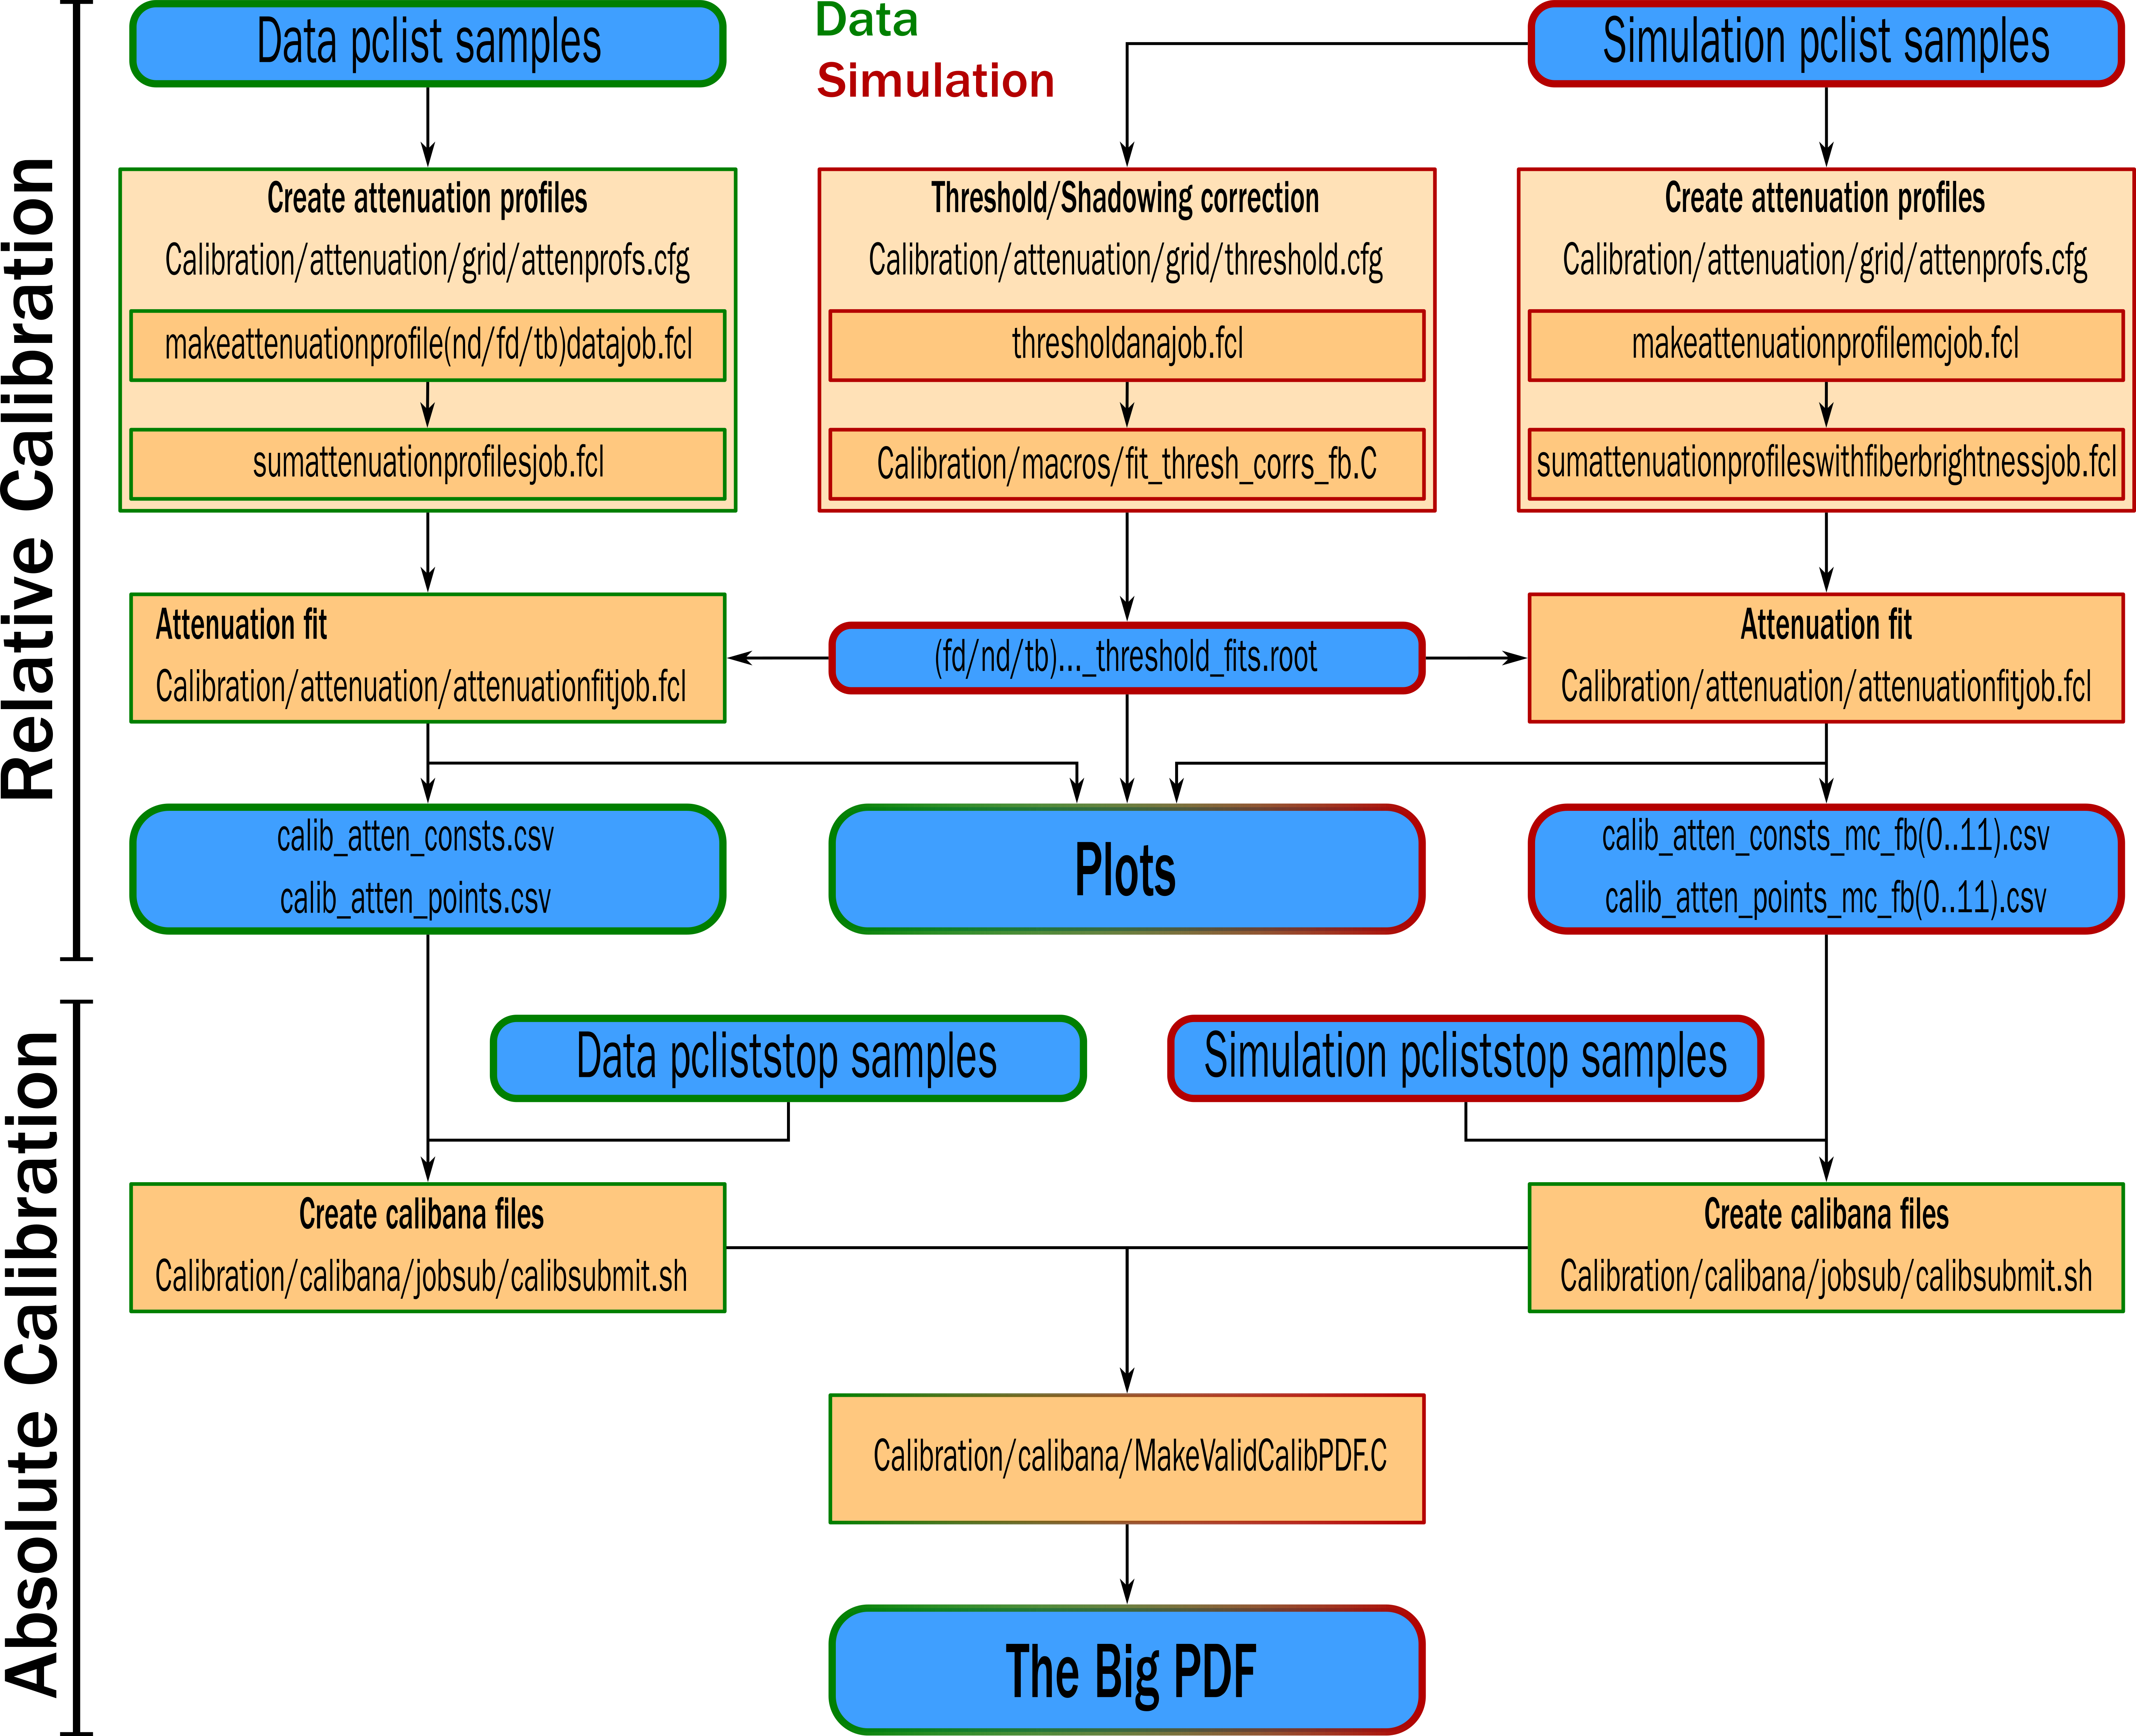
\includegraphics[width=\textwidth]{Plots/CalibrationFlowChart.png}
\caption{Flow chart showing the jobs (orange background) and files (blue background) needed and produced during the full NOvA calibration process. The left chain is showing the data calibration process (with green border) and is applied to every data calibration sample separately (periods or epochs). The center and right chains are showing the simulation calibration proces, which is redone only if there's a change to the detector simulation. The absolute calibration at the bottom combines data and simulation. The entire process is done separately for each NOvA detector.} 
\end{figure}

\subsection{Creating calibration samples}
How do we create the calibration samples and what cuts are applied?

Mention exactly the name and the location of the fcl files to create the TB pclist/pcliststop files. (Or should I only do this in the next section when mentioning the TB calibration?)

What are the main variables that are in the calibration samples? Specifically the PE and such.

When should I talk about the ADC to PE conversion? Here?

\begin{figure}[hbtp]
\centering
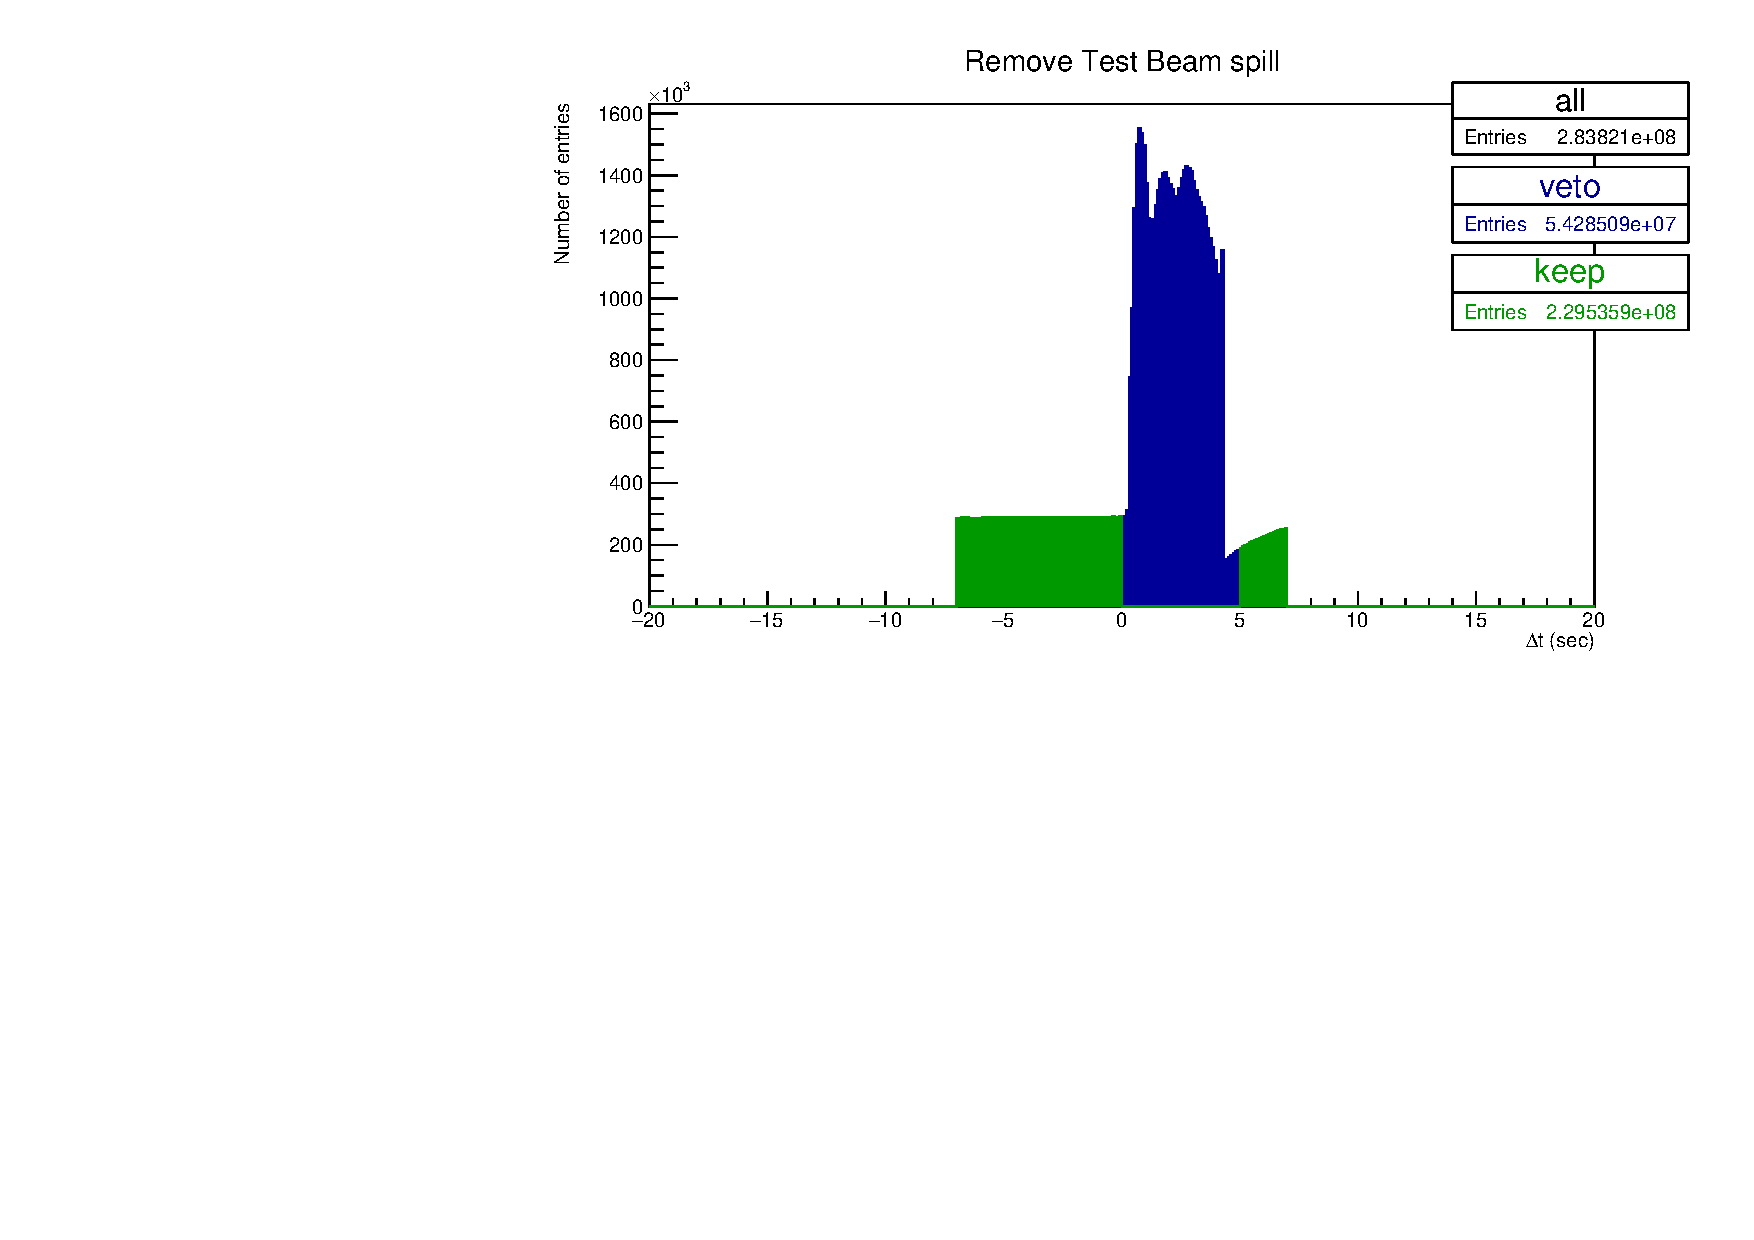
\includegraphics[width=\textwidth]{Plots/RemoveTBSpills.pdf}
\caption{Test Beam beam spill events removed from the calibration samples. Test Beam beam spill is 4.2 seconds long and we remove events (in blue) within a 5 seconds window from the start of the beam spill. The remaining events (green) should mostly consist of cosmic particles. This example and the numbers of entries are for the full period 4 Test Beam sample.}
\end{figure}

\subsubsection*{Tricell condition}
\begin{figure}[hbtp]
\centering
\begin{subfigure}[b]{0.49\textwidth}
\centering
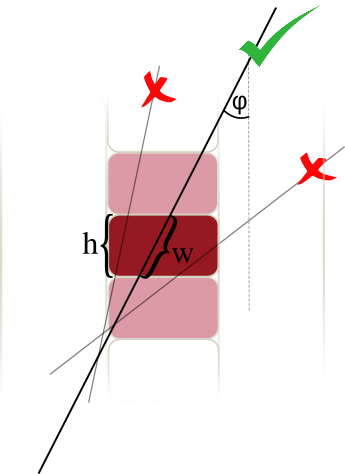
\includegraphics[width=0.6\textwidth]{Plots/TricellConditionWithDescription.png}
\caption{}
\end{subfigure}
\begin{subfigure}[b]{0.49\textwidth}
\centering
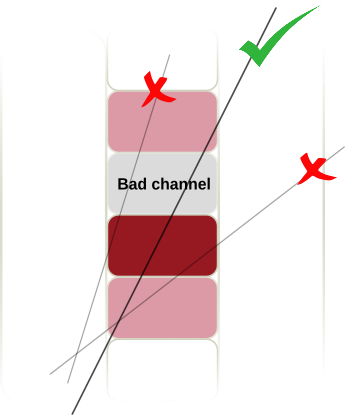
\includegraphics[width=0.6\textwidth]{Plots/TricellConditionWithBadChannel.png}
\caption{}
\end{subfigure}
\caption{Illustration of the tricell condition (a). We only use hits that have two surrounding hits in the same plane to be used in the NOvA calibration. This is to ensure a good quality of the pathlength (w) reconstruction, which is calculated from the known cell height (h) and the reconstructed track angle $\left(\varphi\right)$. In case the hit is next to a bad channel (b), we ignore this bad channel and require a hit in the next cell over.}
\label{figCalibrationFlowchart}
\end{figure}

Adding the underfilled cells to the bad channels which are automatically skipped for the tricell condition

\subsection{Relative calibration}

Detailed description can be found in the "Instructions for the Attenuation Calibration Job" technote from Prabhjot from docdb:13579 (list of all calibration technotes).

Relative calibration/attenuation correction (the exact commands are shown on figure \ref{figCalibrationFlowchart}.
\begin{enumerate}
\item Create the threshold/shadowing corrections
\item Create profile histograms of PE/cm over w for each cell in each plane. The job is \texttt{makeattenuationprofileXjob.fcl}, where \texttt{X} is \texttt{nddata}, \texttt{fddata}, \texttt{tbdata}, or \texttt{mc}.
\item Analyse the calibhist files and draw the histograms
\item Do the attenuation fit using the \texttt{attenuationfitjob.fcl}
\end{enumerate}

Create attenuation profiles
Attenutation profiles have a constant binnin fNBins=100 (in w), same for ND, FD and TB. This results in an effectively finer binning for TB compared to ND and FD. For FD w = (-900,+900), ND: (-250,+250), TB: (-150,+150).
TB: 3cm/bin, ND: 5cm/bin, FD: 18cm/bin.
What effect could this have on the relative calibration results? Particularly on the calibration shape?

Apply the threshold/shielding correction.

Do the fit. What exact fits are we using and in what order? Exponential, fit to residuals...

Now we have the relative calibration done and the constants saves. What are the const and points files that we get? What do they mean?

\subsection{Absolute calibration}

Apply cuts and get an average PECorr response for each epoch/period individually and for each view. Get an average over the two views.

Save the results.

\subsection{Calibration uncertainties}


%%%%%%%%%%%%%%%%%%%%%%%%%%%%%%%%%%%%%%%%%%%%%%%%%%%%%%%%%%%%%%%%%%%%%%%%%%%%%%%
%%%%%%%%%%%%%%%%%%%%%%%%%%%%%%%%%%%%%%%%%%%%%%%%%%%%%%%%%%%%%%%%%%%%%%%%%%%%%%%
%%%
%%%                      Test Beam calibration description
%%%
%%%%%%%%%%%%%%%%%%%%%%%%%%%%%%%%%%%%%%%%%%%%%%%%%%%%%%%%%%%%%%%%%%%%%%%%%%%%%%%
\section{NOvA Test Beam detector calibration}
\subsection{Overview}
History of TB calibration. What led to the final version of TB calibration. What can be done next.

Dates and times when the data taking occured.

From Calibration\_Meta\_READFIRST.pdf:
Validations	of any calibration correction take the same basic form:
\begin{enumerate}
\item What deficency are you correcting for? (For Test Beam this would be the difference between the different scintillators, also the faulty FEBs, distribution of w is not flat, especially in the overfilled cells. The energy response between the different cells and planes is not the same. Maybe I should talk about this for each period separately when I have the calibhist plots which show the non-linearities. Also the PhotonTransport plots don't really show the PECorr but the PE/cm itself but with the fit!!!
\item What correction factors/scales have you found? Show them in plot form. (This is basically the PhotonTransport plots for the relative calibration and the pecorrcm distributions for the absolute calibration)
\item Now generate the same plots as in (1) but with the corrections applied. Technically this is the absolute calibration validation plots. Does this mean that the PE/cm plots from the absolute calibration should be/are exactly the same as the calibhist plots? Not entirely as those are only for the stopping muons, whereas the calibhist are for the through-going muons. Does it mean I should maybe generate the calibhist plots with the relative calibration applied?
\item Ratios of plots in (3) to (1) to highlight any patterns or difficult-to-spot discrpancies between what we think should happen when the constants are applied, and what does happen. But what does this tell us? It's basically just an average of the attenuation correction...
\end{enumerate}


Period naming, possibly epochs (for P3).
List of data samples, plus MC samples that were used and pointer to the data-based simulation technote.
%Possibly refer to https://cdcvs.fnal.gov/redmine/projects/novatestbeam/wiki/Period_and_Epoch_Naming

Specific running conditions: - maybe enough to mention this in the individual descriptions of the test beam periods
Underfilled cells
Faulty FEBs (Period 2 and Period 3)

Why do we do the calibration generally and why do we need to do in for Test Beam specifically - probably in the introduction

Temperature study (small overview)

From Teresa's thesis
Along with setting the energy scale of the detector, we need to calibrate the timing of the readout system for the detector. The Data Concentrator Modules (DCMs) responsible for collating the data from multiple FEBs get their timing information via a daisy chain originating at the detector TDU. Each DCM in the chain has a timing offset relative to the DCM before it, with the last DCM having the earliest ti. Following the procedure described in [66], I used timing information from hits on cosmic ray muon tracks that pass through multiple DCMs to determine the relative offsets between DCMs, shown in Figure 3.20.

\subsubsection{Definitions}
List all final data and simulation definitions used.

From Teresa's thesis:
"For Test Beam, we have three beam-based triggers, one pulsed trigger, and two data-driven triggers. The data-driven triggers are both activity-based triggers. The first is intended to record cosmic ray induced events for use in calibrating the detector.

\subsection{Detector Brightness}

\begin{figure}[hbtp]
\centering
\begin{subfigure}[b]{0.495\textwidth}
\centering
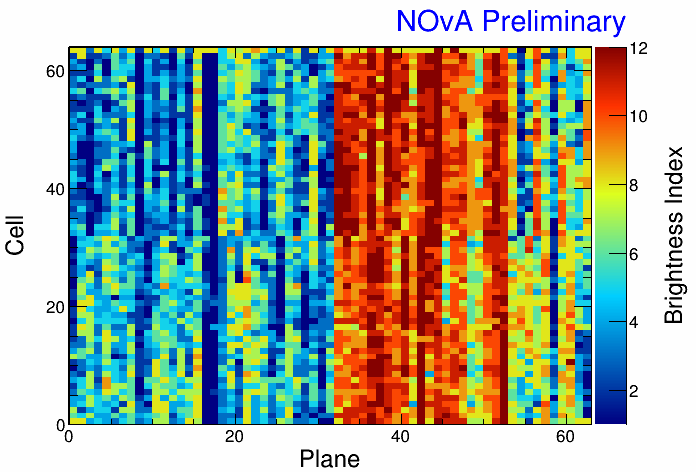
\includegraphics[width=\textwidth]{Plots/BrightnessIndex.png}
\end{subfigure}
%\hfill
\begin{subfigure}[b]{0.495\textwidth}
\centering
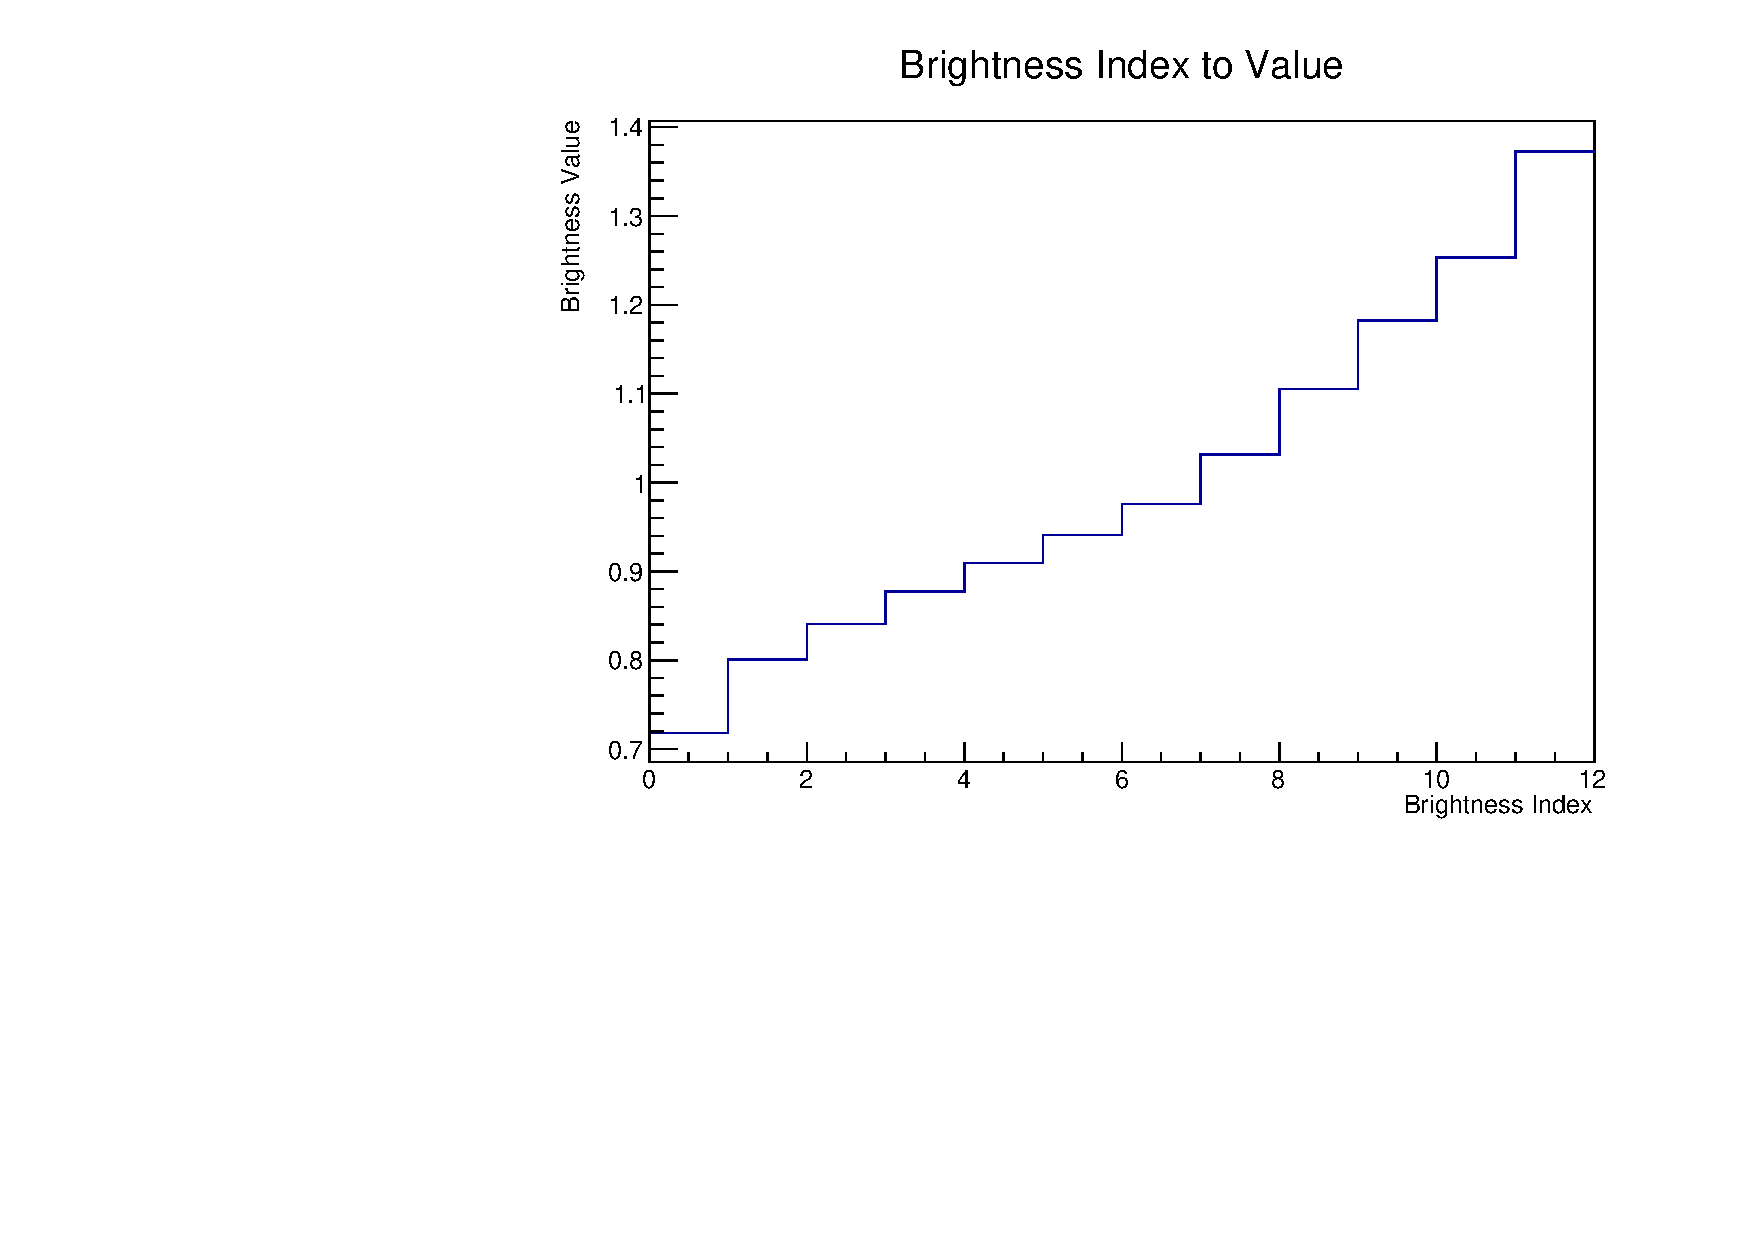
\includegraphics[width=\textwidth]{Plots/BrightnessIndexToValue.pdf}
\end{subfigure}
\caption{The Test Beam detector is (like the standard NOvA detectors) divided into 12 brightness bins (left plot), each representing a relative difference in energy response (right plot) due to different brightnesses of the fibers, scintillators, or readout.}
\end{figure}

\subsection{Simulation}

We originally used Teresa's calibration MC sample, but after we saw disagreement, we developed a new MC based off of the period 3 data, which we ended up using for both period 2 and period 3. For fibre brightness we are also using the same MC from period 3 data as it represents the detector in its best condition.

We used a data-based simulation of cosmic muons for the Test Beam detector calibration. The details are described in the technote XXX. We used this and this data as a basis and this and this data for the fiber brighness file.

\begin{figure}[!hbtp]
\centering
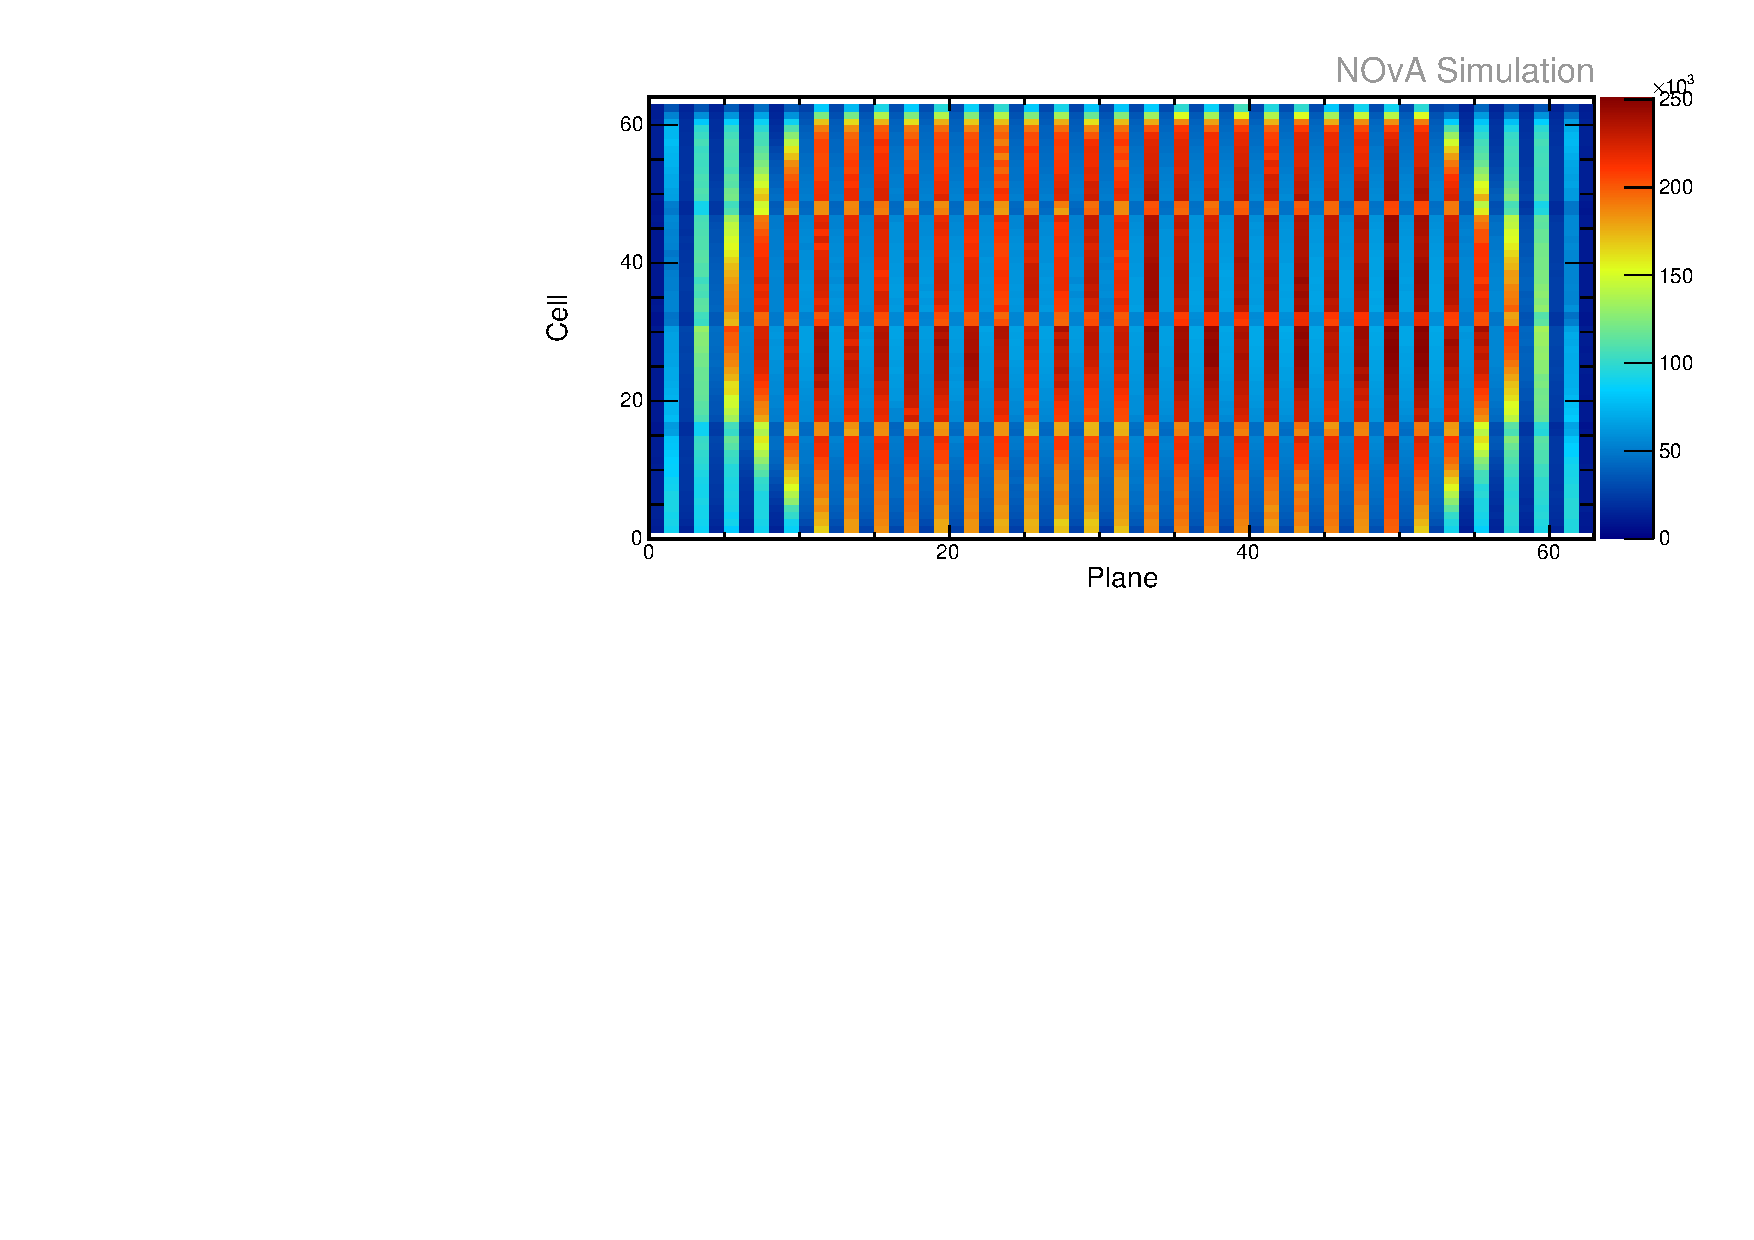
\includegraphics[width=\textwidth]{Plots/Attenprofs_Simulation_CellPlane.pdf}
\caption{Distribution of events in the Test Beam simulation calibration sample.}
\end{figure}

\subsubsection{Relative calibration results}
\begin{figure}[!hbtp]
\centering
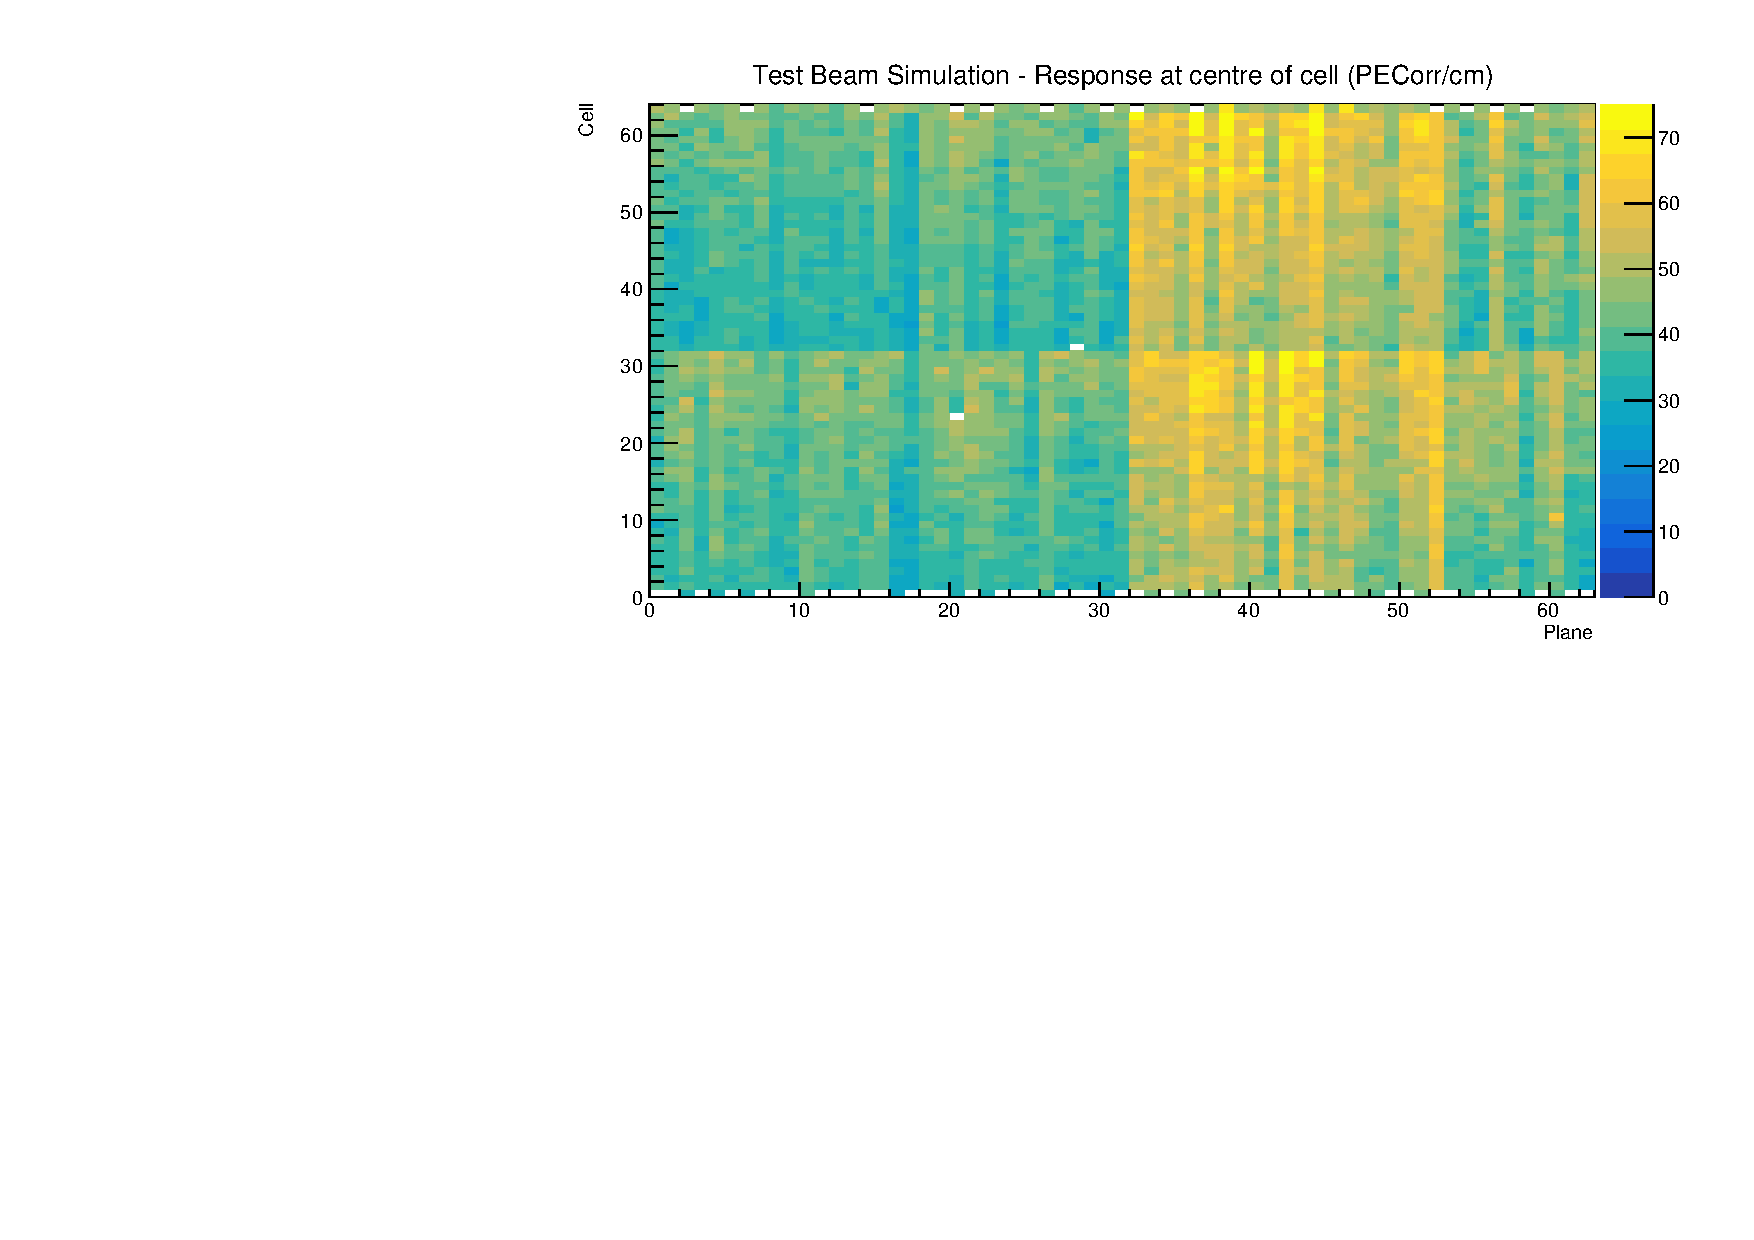
\includegraphics[width=\textwidth]{Plots/CellResponseAtCentre_Prod4DataBasedSim.pdf}
\caption{Overview of the relative calibration results for the Teast Beam detector simulation. Each cell is represents the average corrected energy response (in PECorr/cm) in the centre of each cell. The blank cells are uncalibrated.}
\end{figure}

\subsection{Period 1}
Only a month of data, only first half of detector filled, primary/secondary beam halo, or oversaturation leading to FEB shutoffs [docdb:38349 and 41331].
Only used for comissioning, not used for any data analysis or calibration.

\subsection{Period 2}
What was done for the period 2 tb calibration, short overview of what has been done: test beam data were calibrated all at the same time without splitting them to separate epochs. See figures \ref{figCalibhistWPE_period2},\ref{figCalibhistCellPE_period2} and \ref{figCalibhistPlanePE_period2}.

\begin{figure}[!hbtp]
\centering
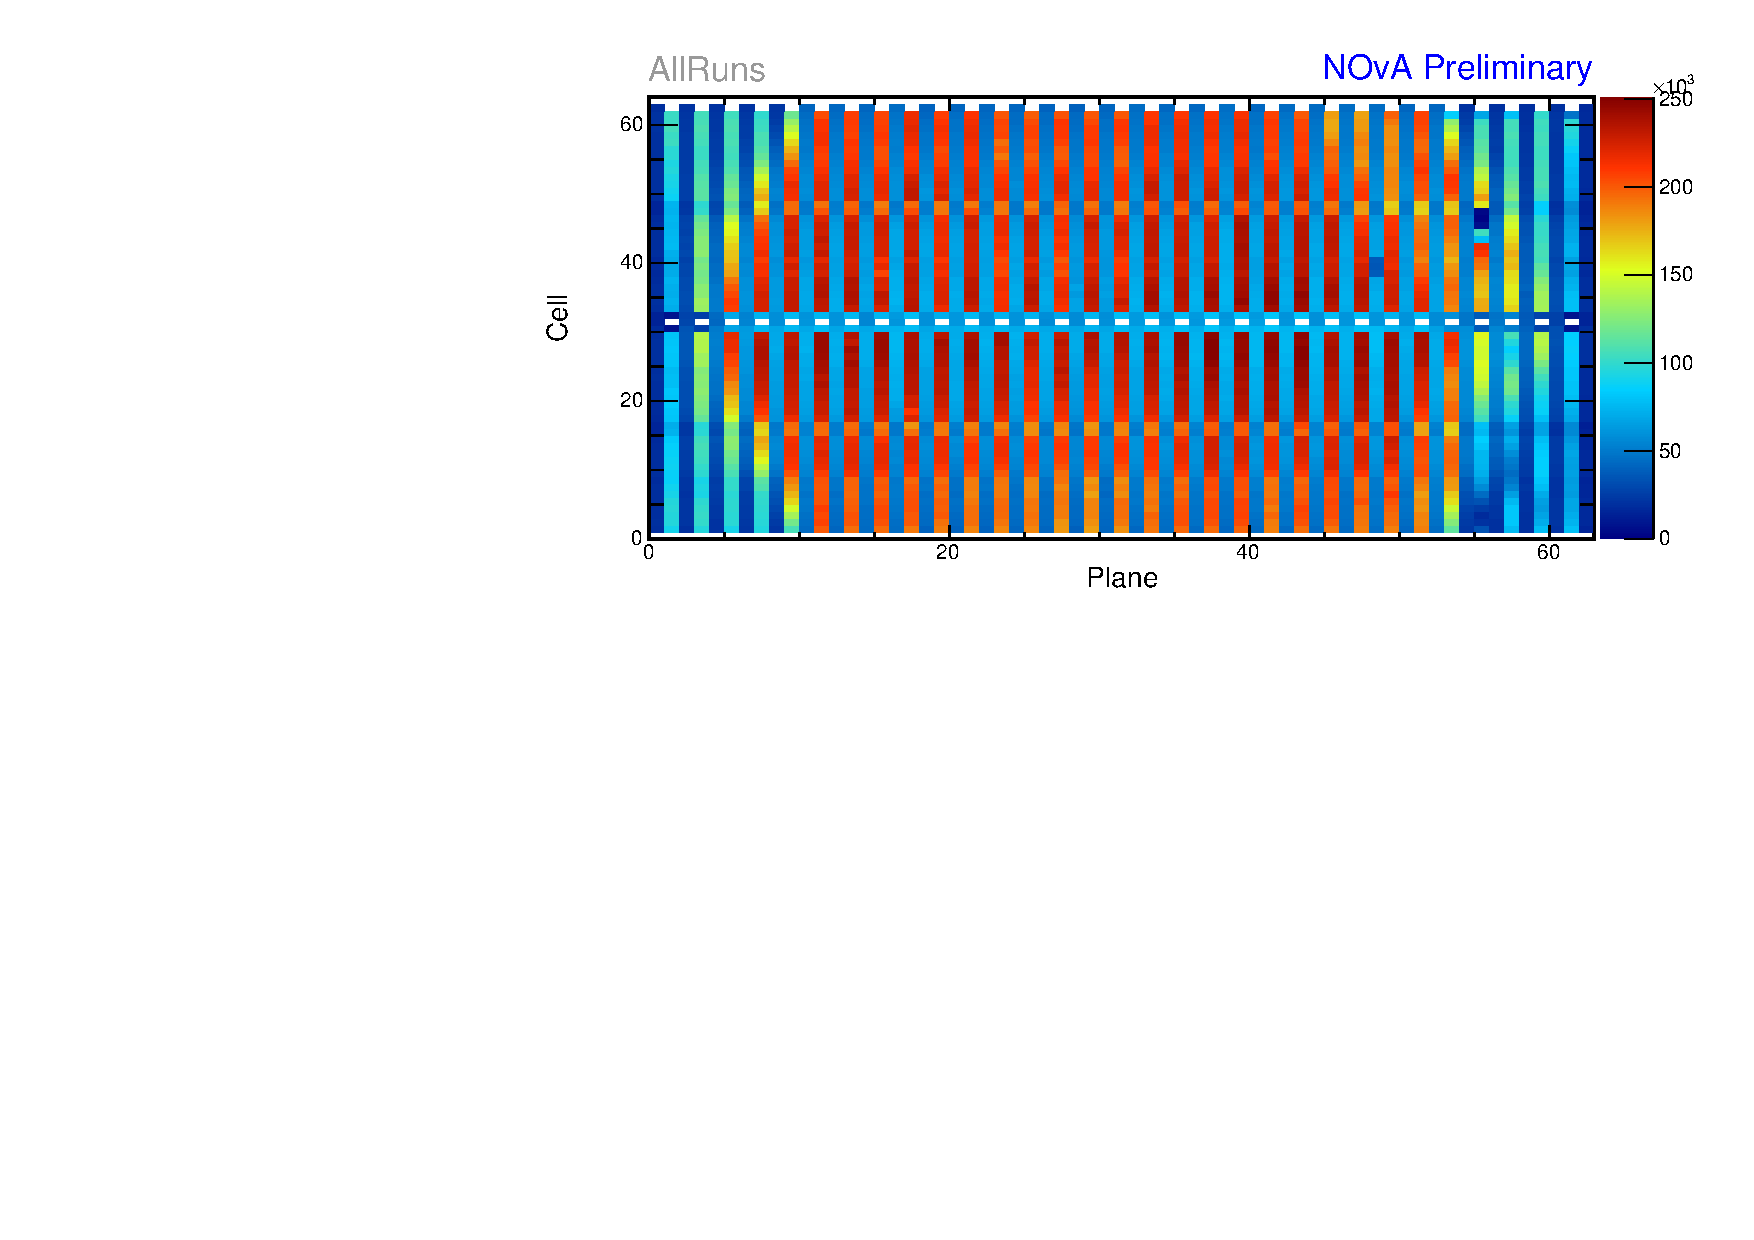
\includegraphics[width=0.9\textwidth]{Plots/Attenprofs_P2Data_CellPlane_AllRuns.pdf}
\caption{Distribution of events in the period 2 Test Beam data calibration sample.}
\end{figure}

\begin{figure}[!hbtp]
\centering
\begin{subfigure}[b]{0.495\textwidth}
\centering
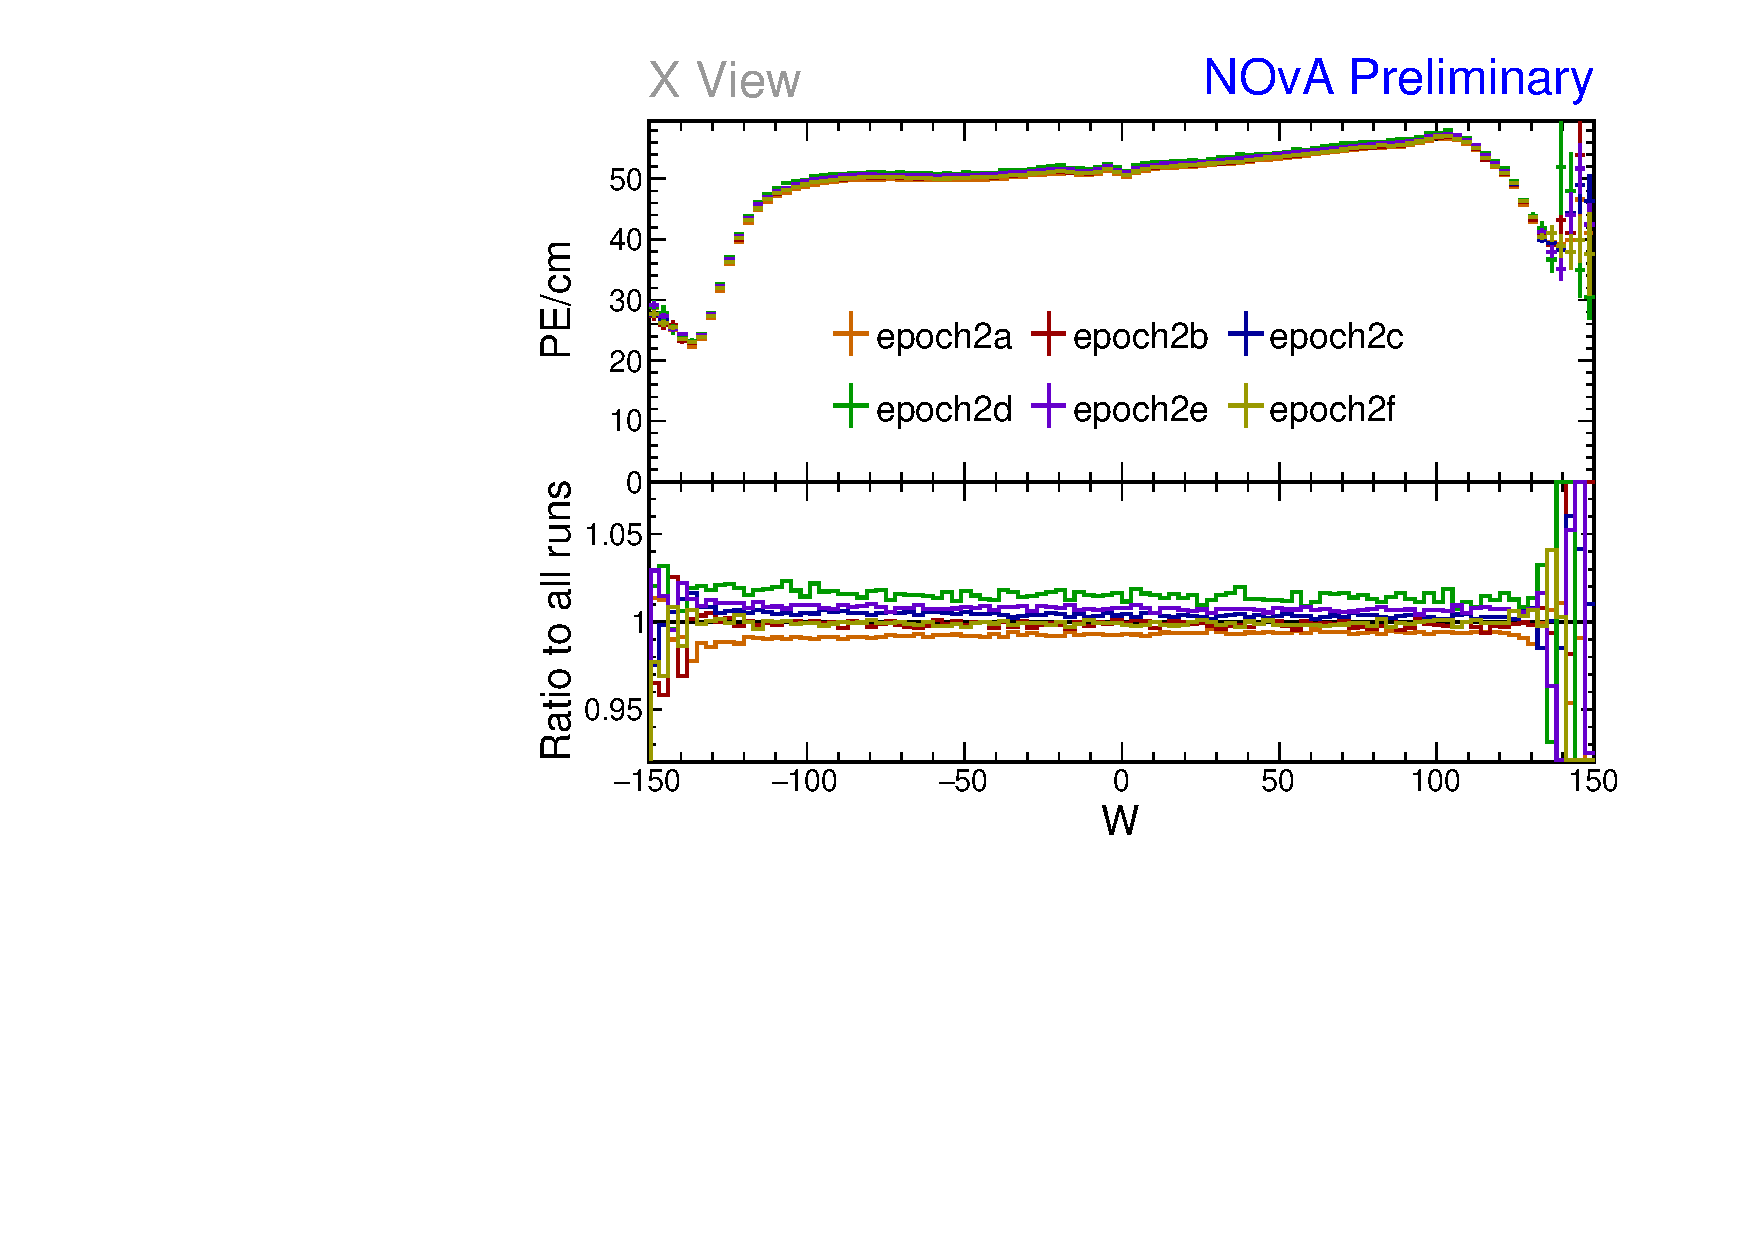
\includegraphics[width=\textwidth]{Plots/Attenprofs_P2Data_WPE_corr_xy_X_Combined.pdf}
\end{subfigure}
\begin{subfigure}[b]{0.495\textwidth}
\centering
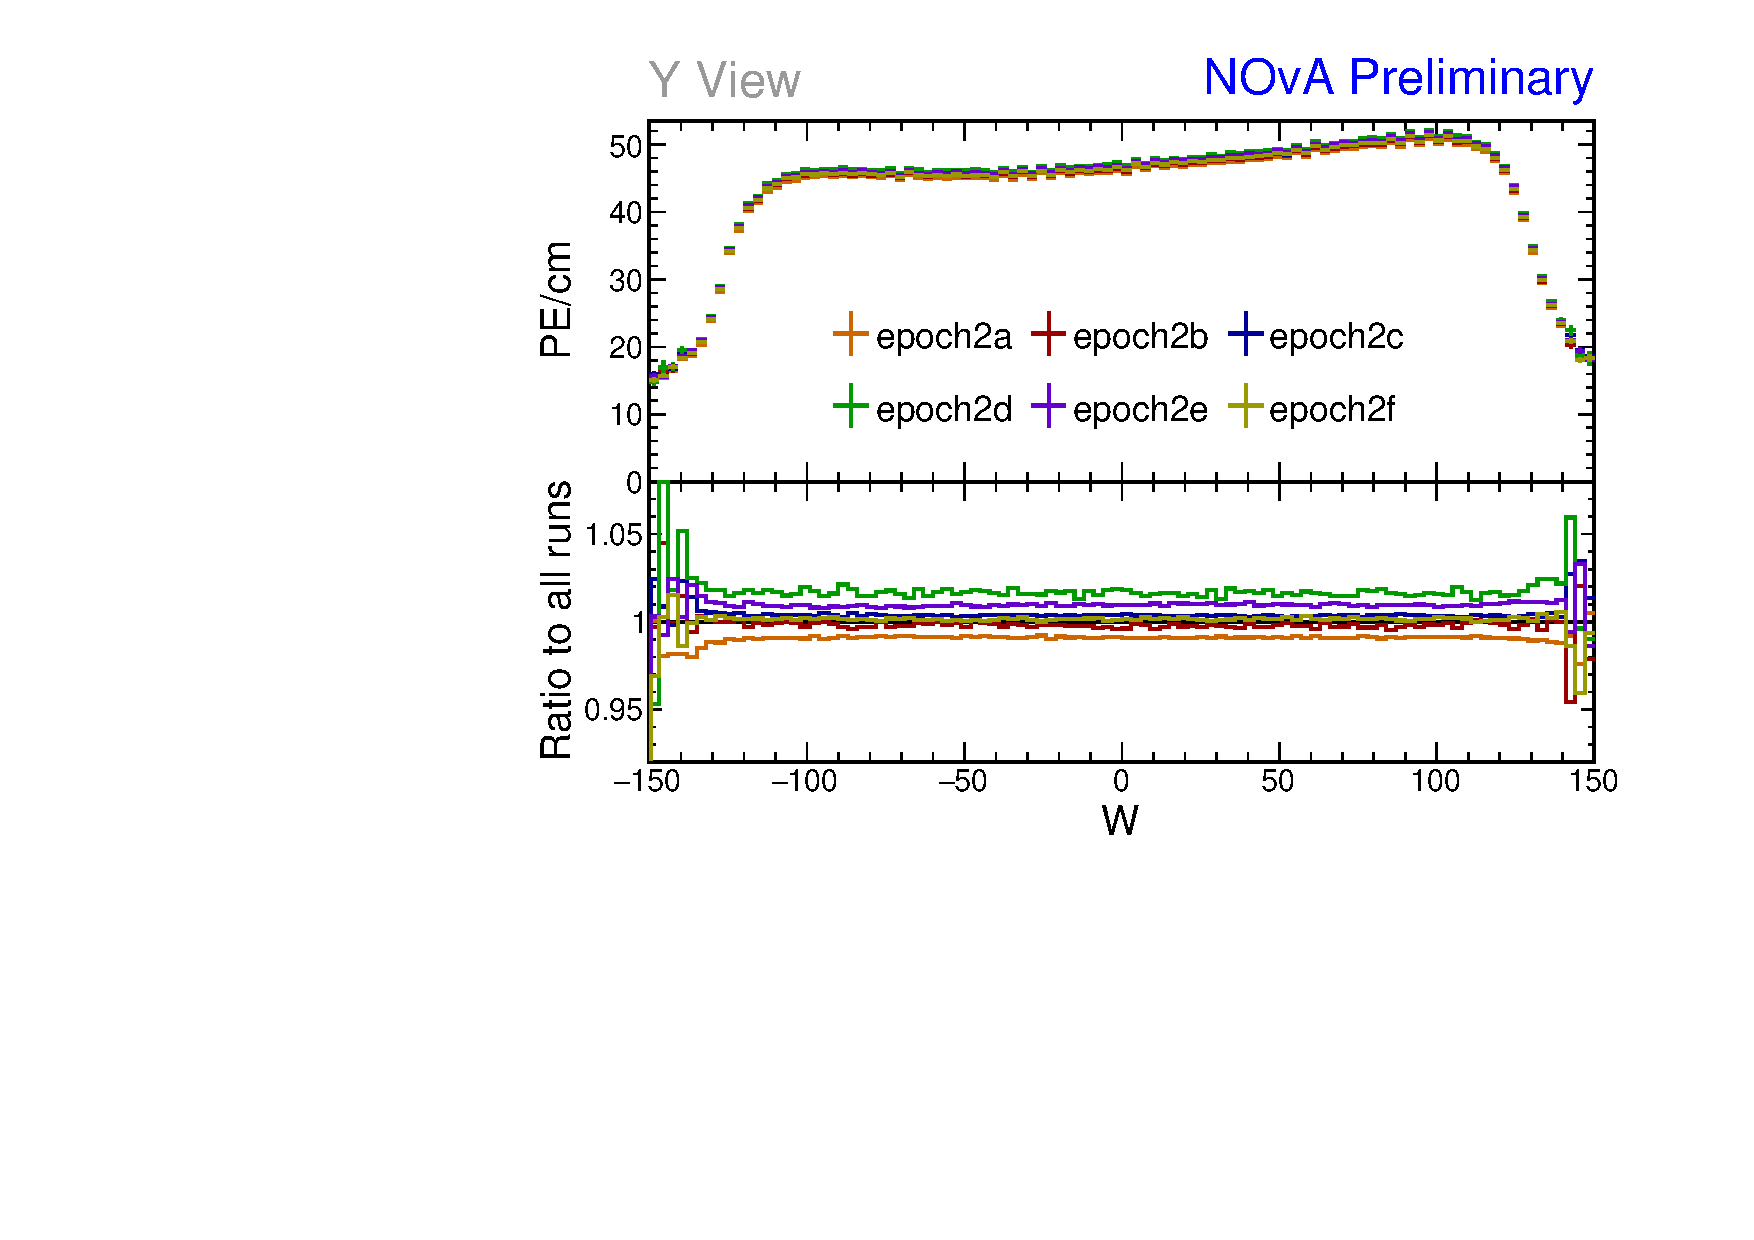
\includegraphics[width=\textwidth]{Plots/Attenprofs_P2Data_WPE_corr_xy_Y_Combined.pdf}
\end{subfigure}
\caption{Uncorrected average energy response as a function of the position within a cell (w) for epochs in period 2. It is clear that there is no significant difference between the various epochs.}
\label{figCalibhistWPE_period2}
\end{figure}

\begin{figure}[!hbtp]
\centering
\begin{subfigure}[b]{0.495\textwidth}
\centering
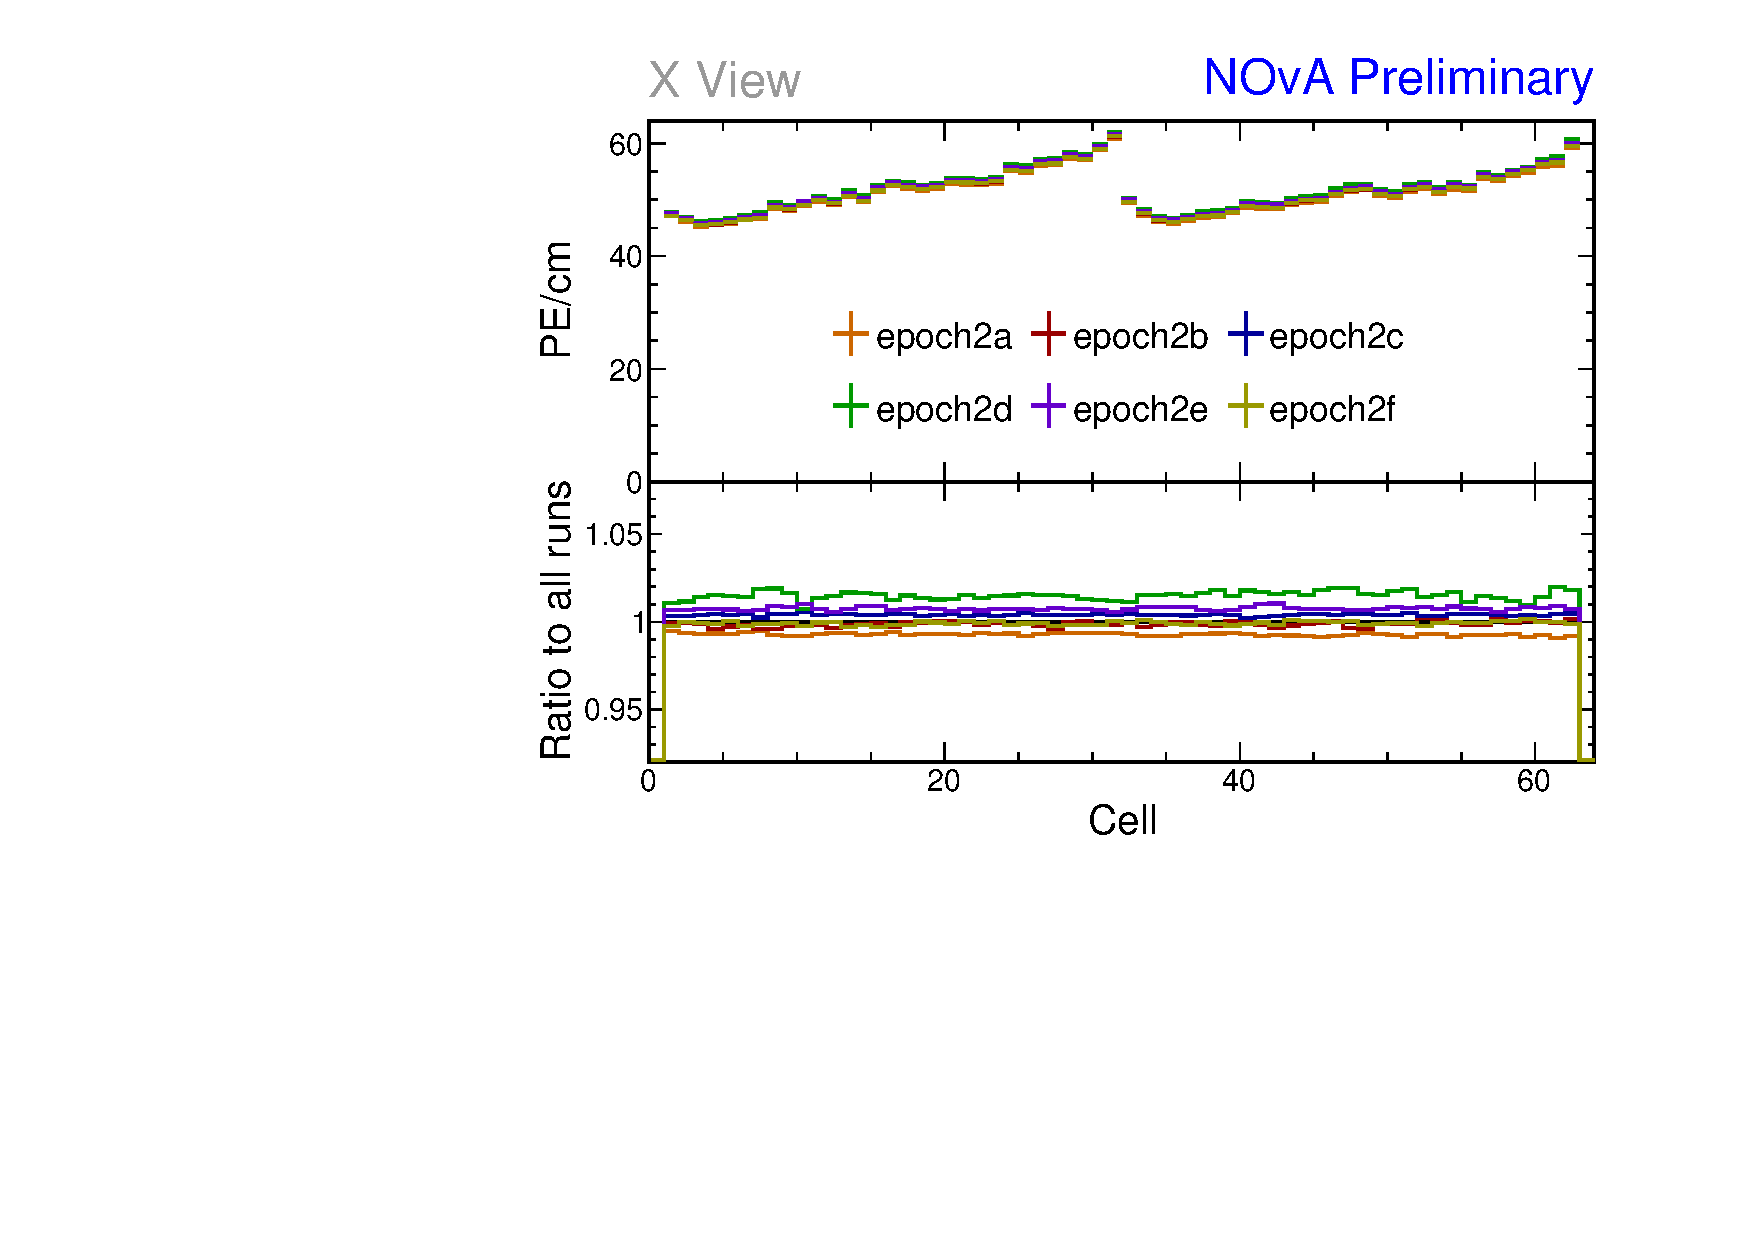
\includegraphics[width=\textwidth]{Plots/Attenprofs_P2Data_CellPE_X_Combined.pdf}
\end{subfigure}
\begin{subfigure}[b]{0.495\textwidth}
\centering
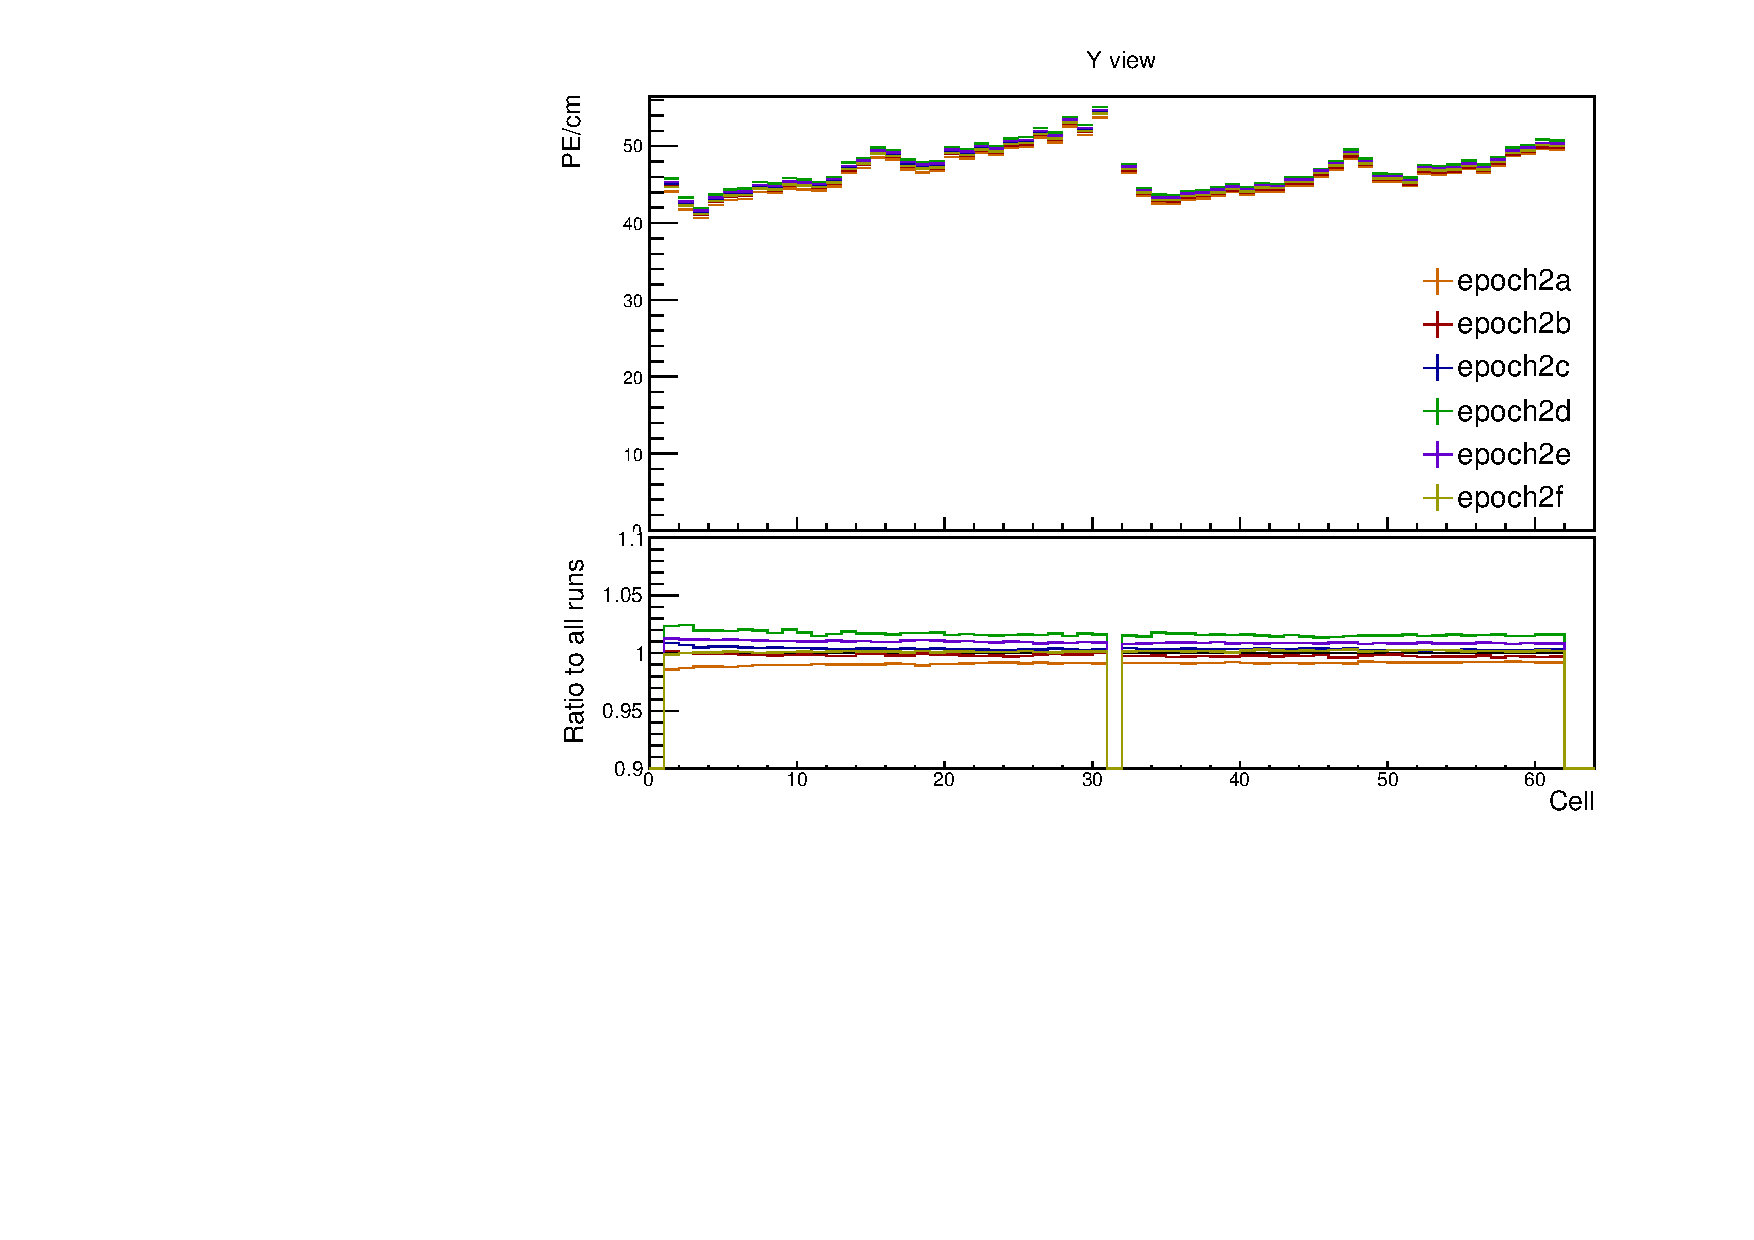
\includegraphics[width=\textwidth]{Plots/Attenprofs_P2Data_CellPE_Y_Combined.pdf}
\end{subfigure}
\caption{Uncorrected average energy response as a function of cells for epochs in period 2.}
\label{figCalibhistCellPE_period2}
\end{figure}

\begin{figure}[!hbtp]
\centering
\begin{subfigure}[b]{0.495\textwidth}
\centering
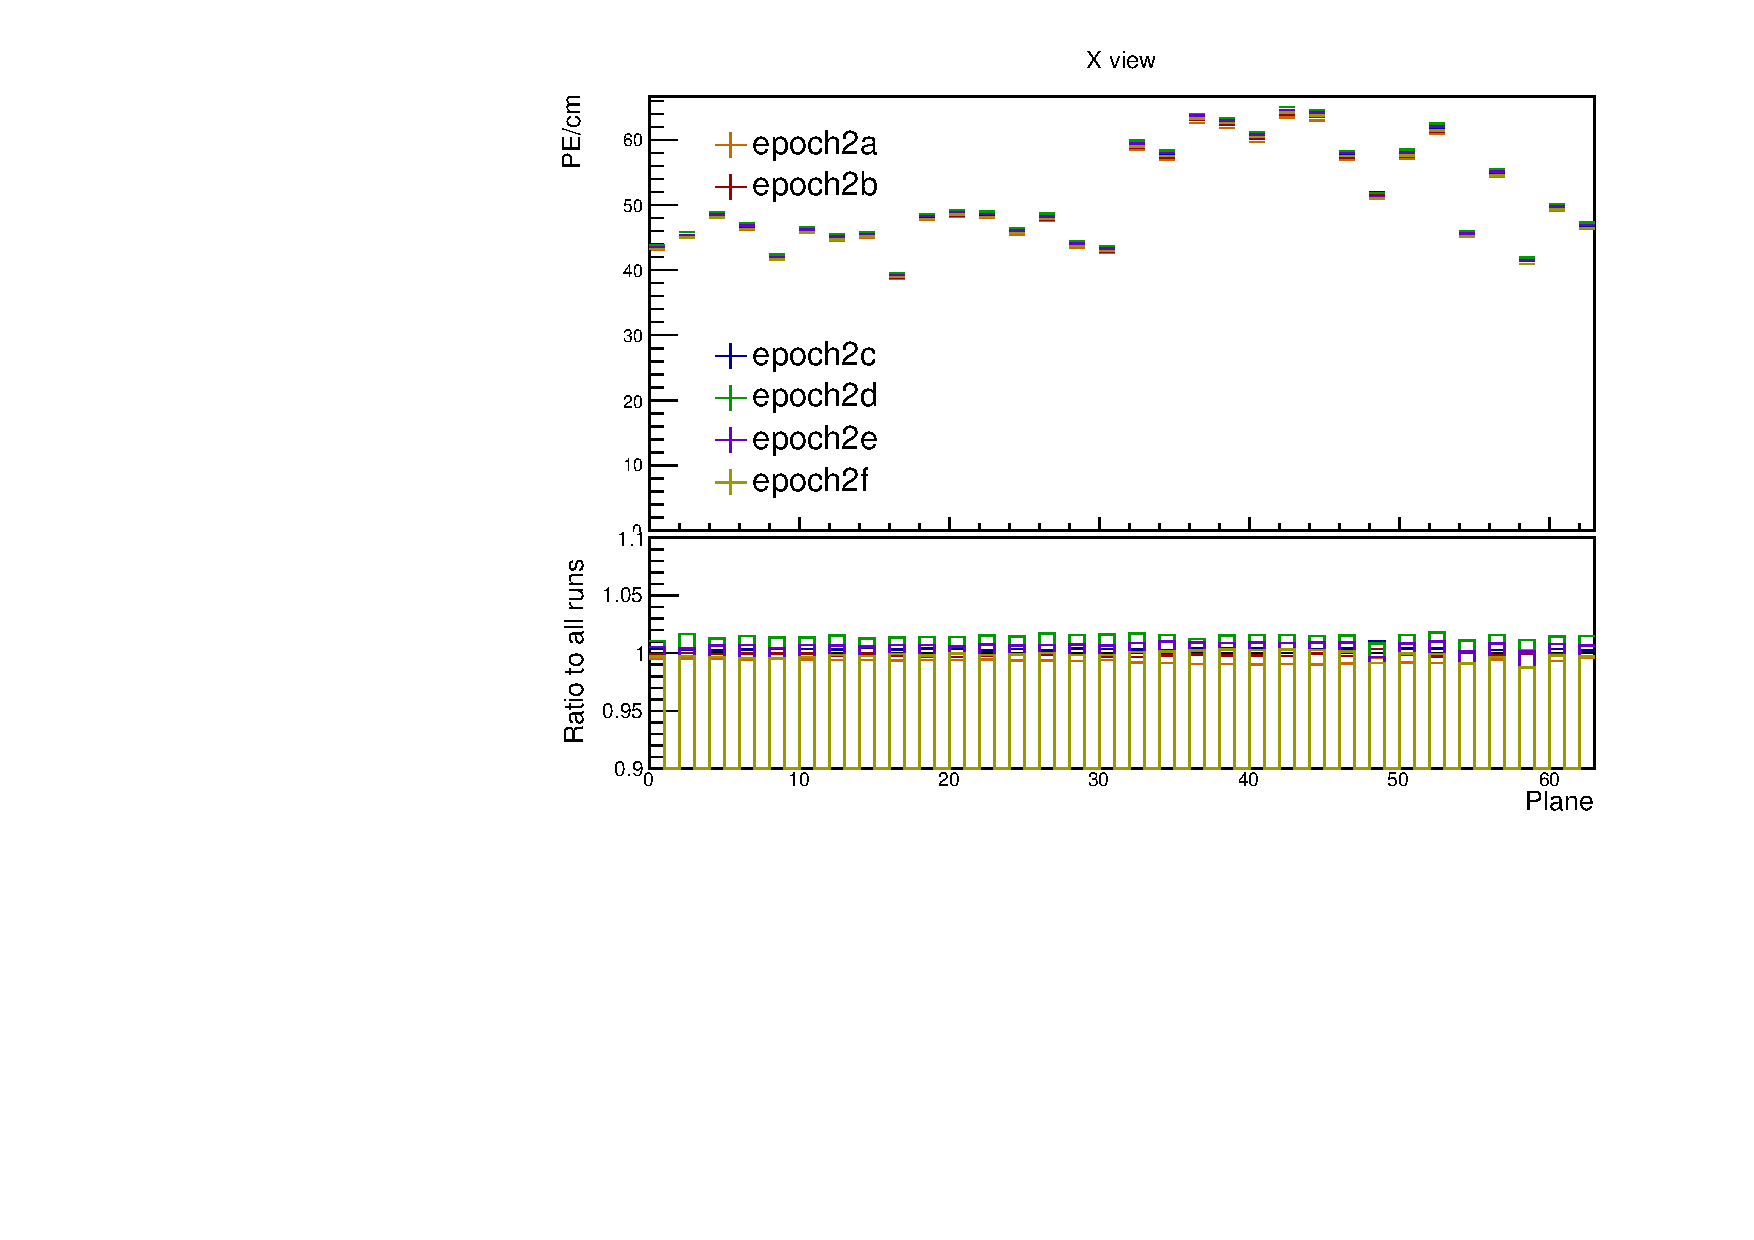
\includegraphics[width=\textwidth]{Plots/Attenprofs_P2Data_PlanePE_X_Combined.pdf}
\end{subfigure}
\begin{subfigure}[b]{0.495\textwidth}
\centering
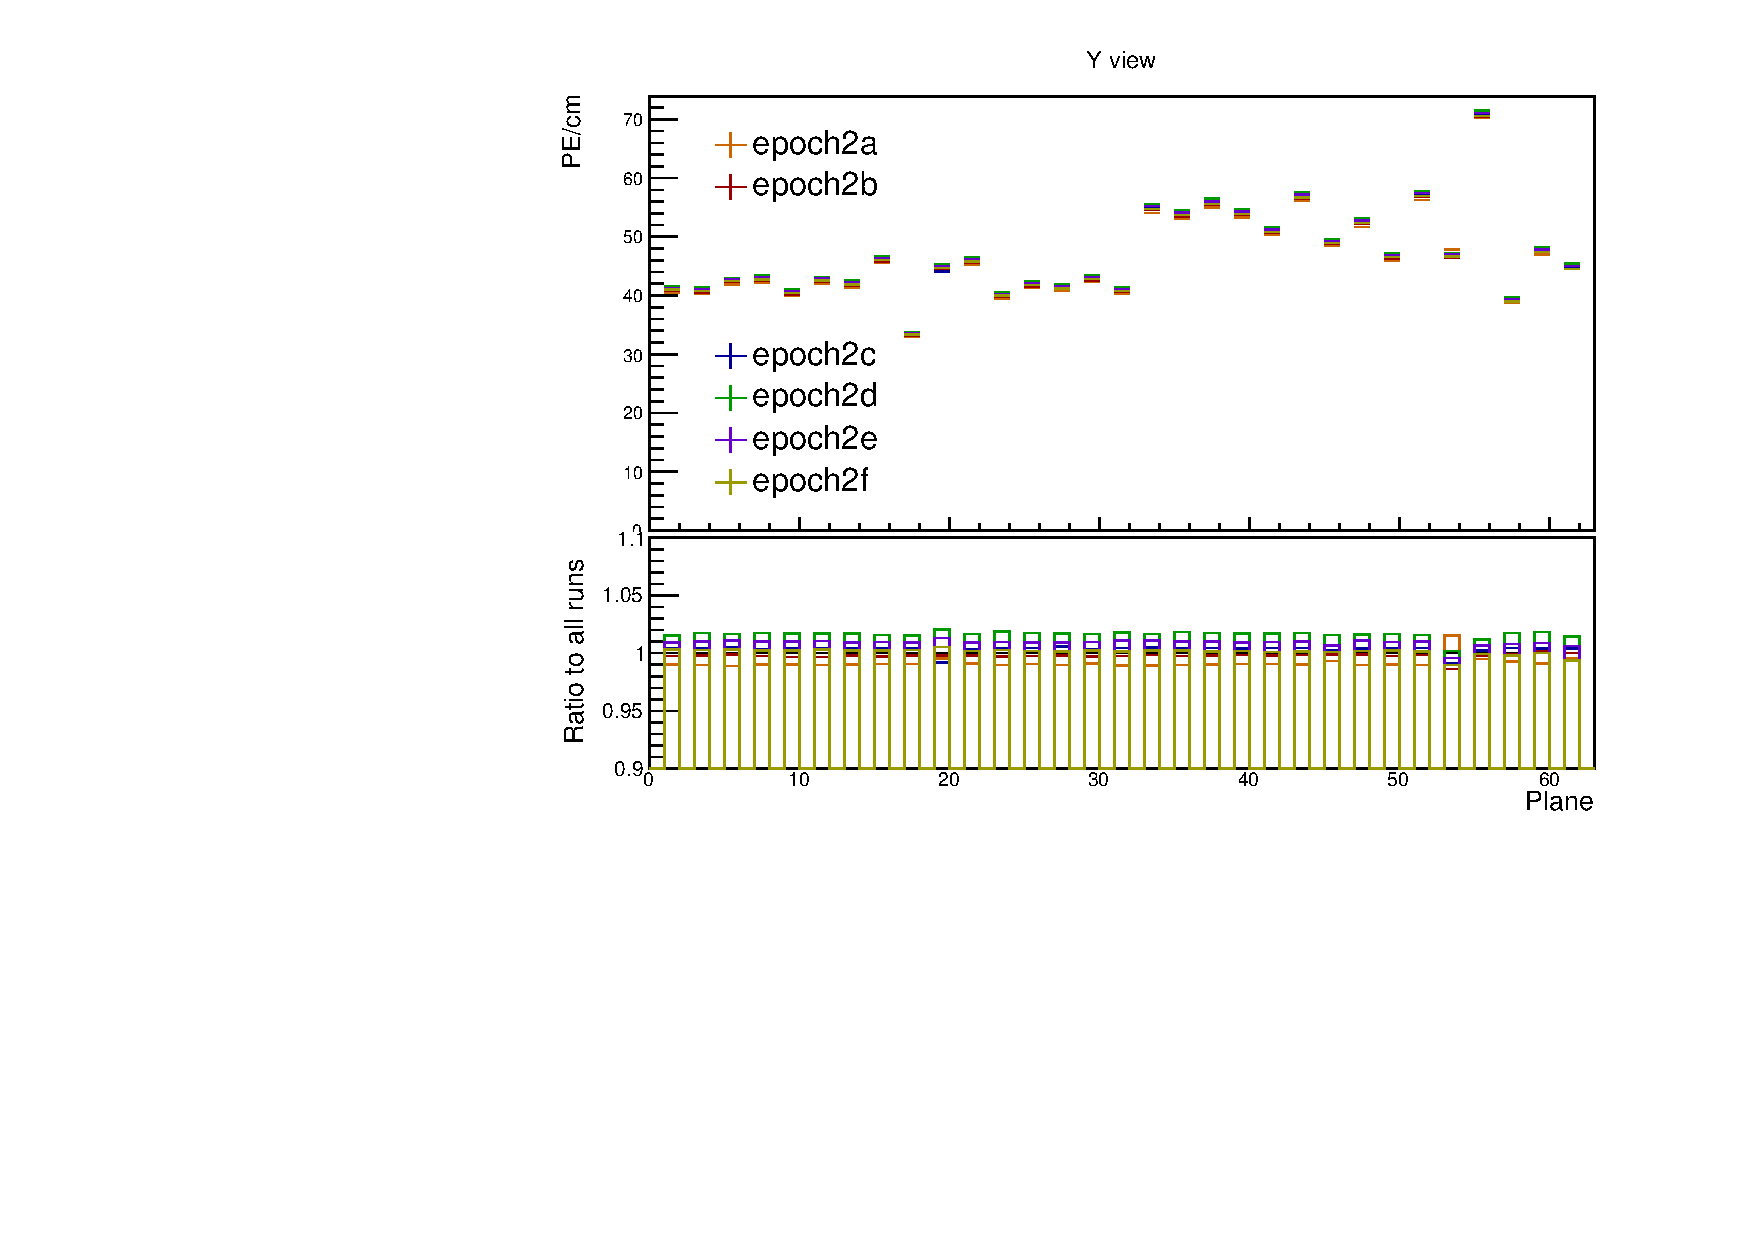
\includegraphics[width=\textwidth]{Plots/Attenprofs_P2Data_PlanePE_Y_Combined.pdf}
\end{subfigure}
\caption{Uncorrected average energy response as a function of planes for epochs in period 2.}
\label{figCalibhistPlanePE_period2}
\end{figure}

\subsubsection{Relative calibration results}

\begin{figure}[!hbtp]
\centering
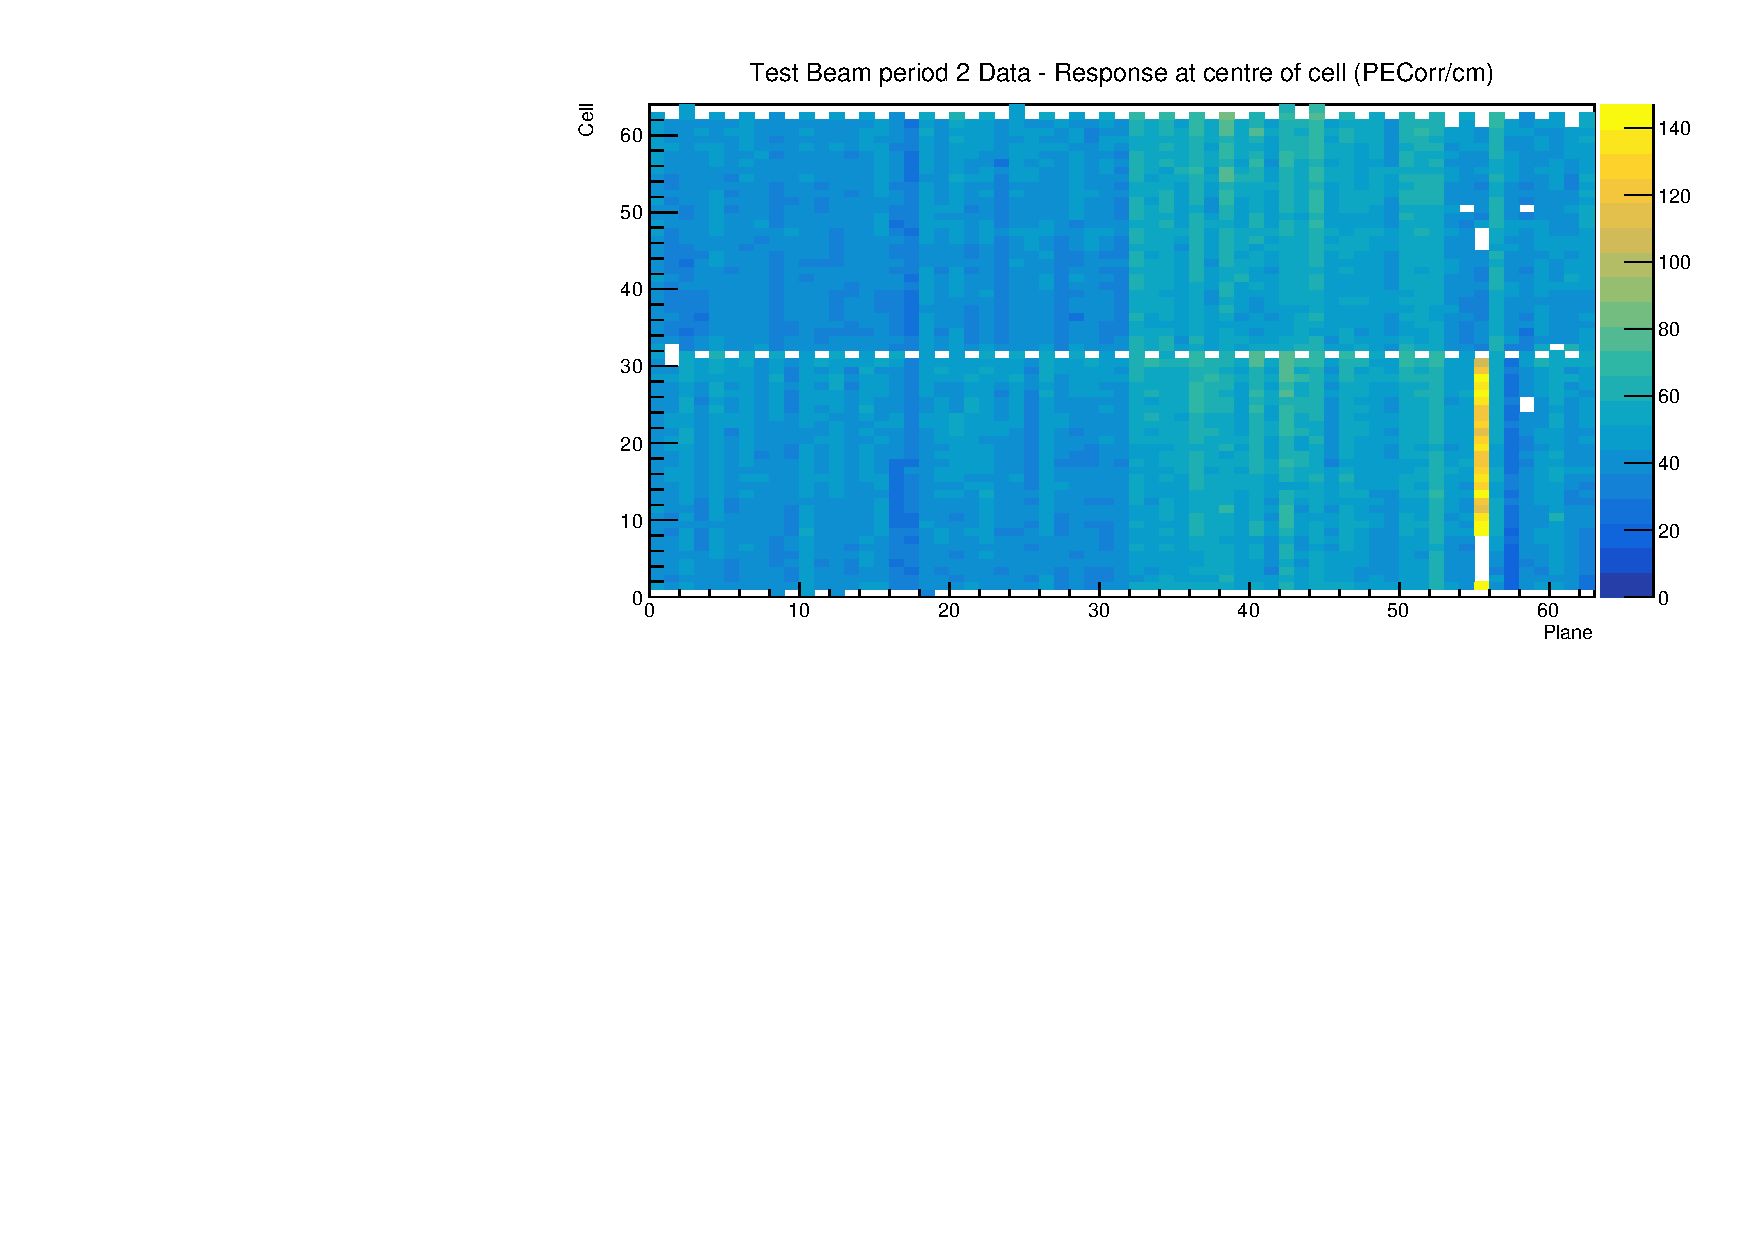
\includegraphics[width=0.9\textwidth]{Plots/CellResponseAtCentre_period2.pdf}
\caption{Overview of the relative calibration results for the Teast Beam detector period 2 data. Each cell is represents the average corrected energy response (in PECorr/cm) in the centre of each cell. The blank cells are uncalibrated.}
\end{figure}

\subsection{Period 3}
Separation of Period 3 data into different epochs based on the running conditions (include plot of the running conditions). We are separating data into pre- and post- filling states. We're using only the fully-refilled post-FEB swap data from period 3 as a basis for the simulation creation.

\begin{figure}[!hbtp]
\centering
\begin{subfigure}[b]{\textwidth}
\centering
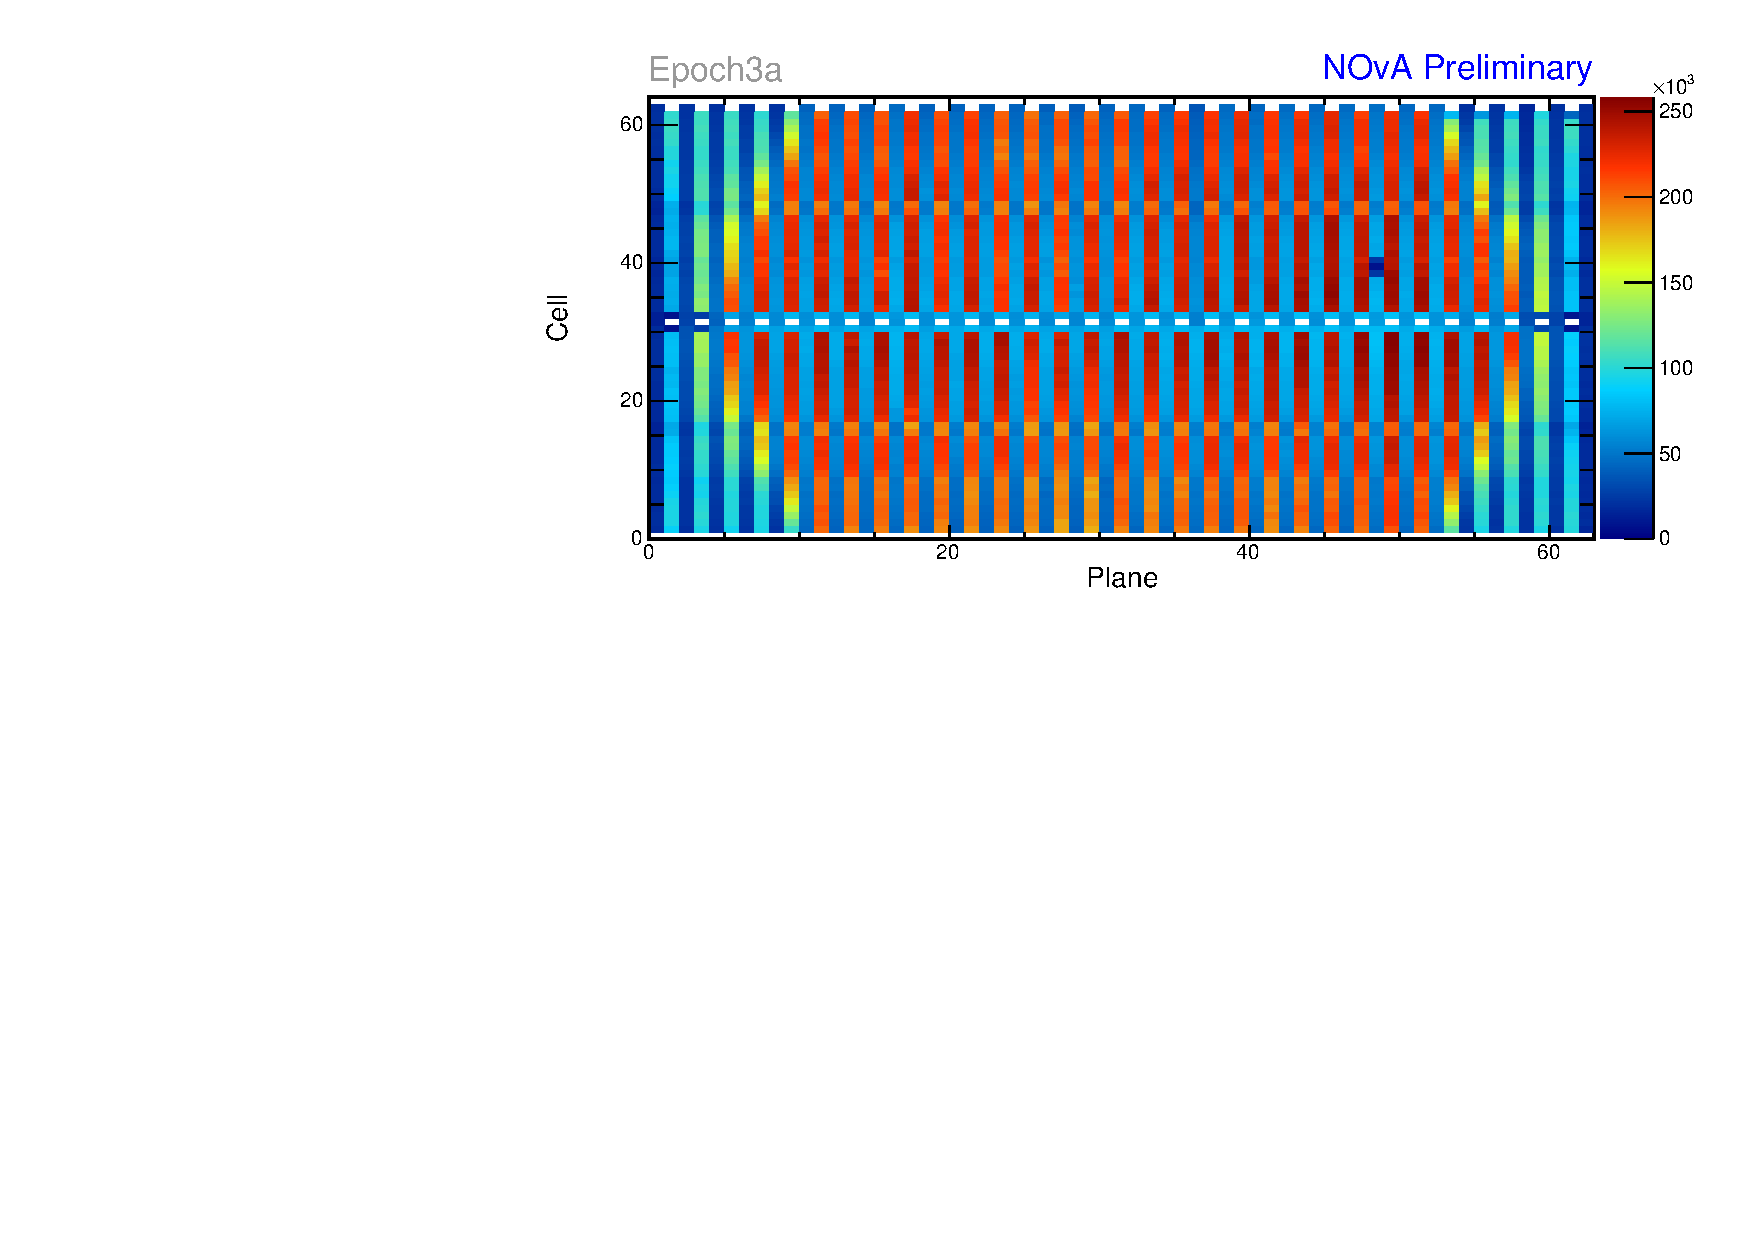
\includegraphics[width=0.9\textwidth]{Plots/Attenprofs_P3Data_CellPlane_Epoch3a.pdf}
\end{subfigure}
\begin{subfigure}[b]{\textwidth}
\centering
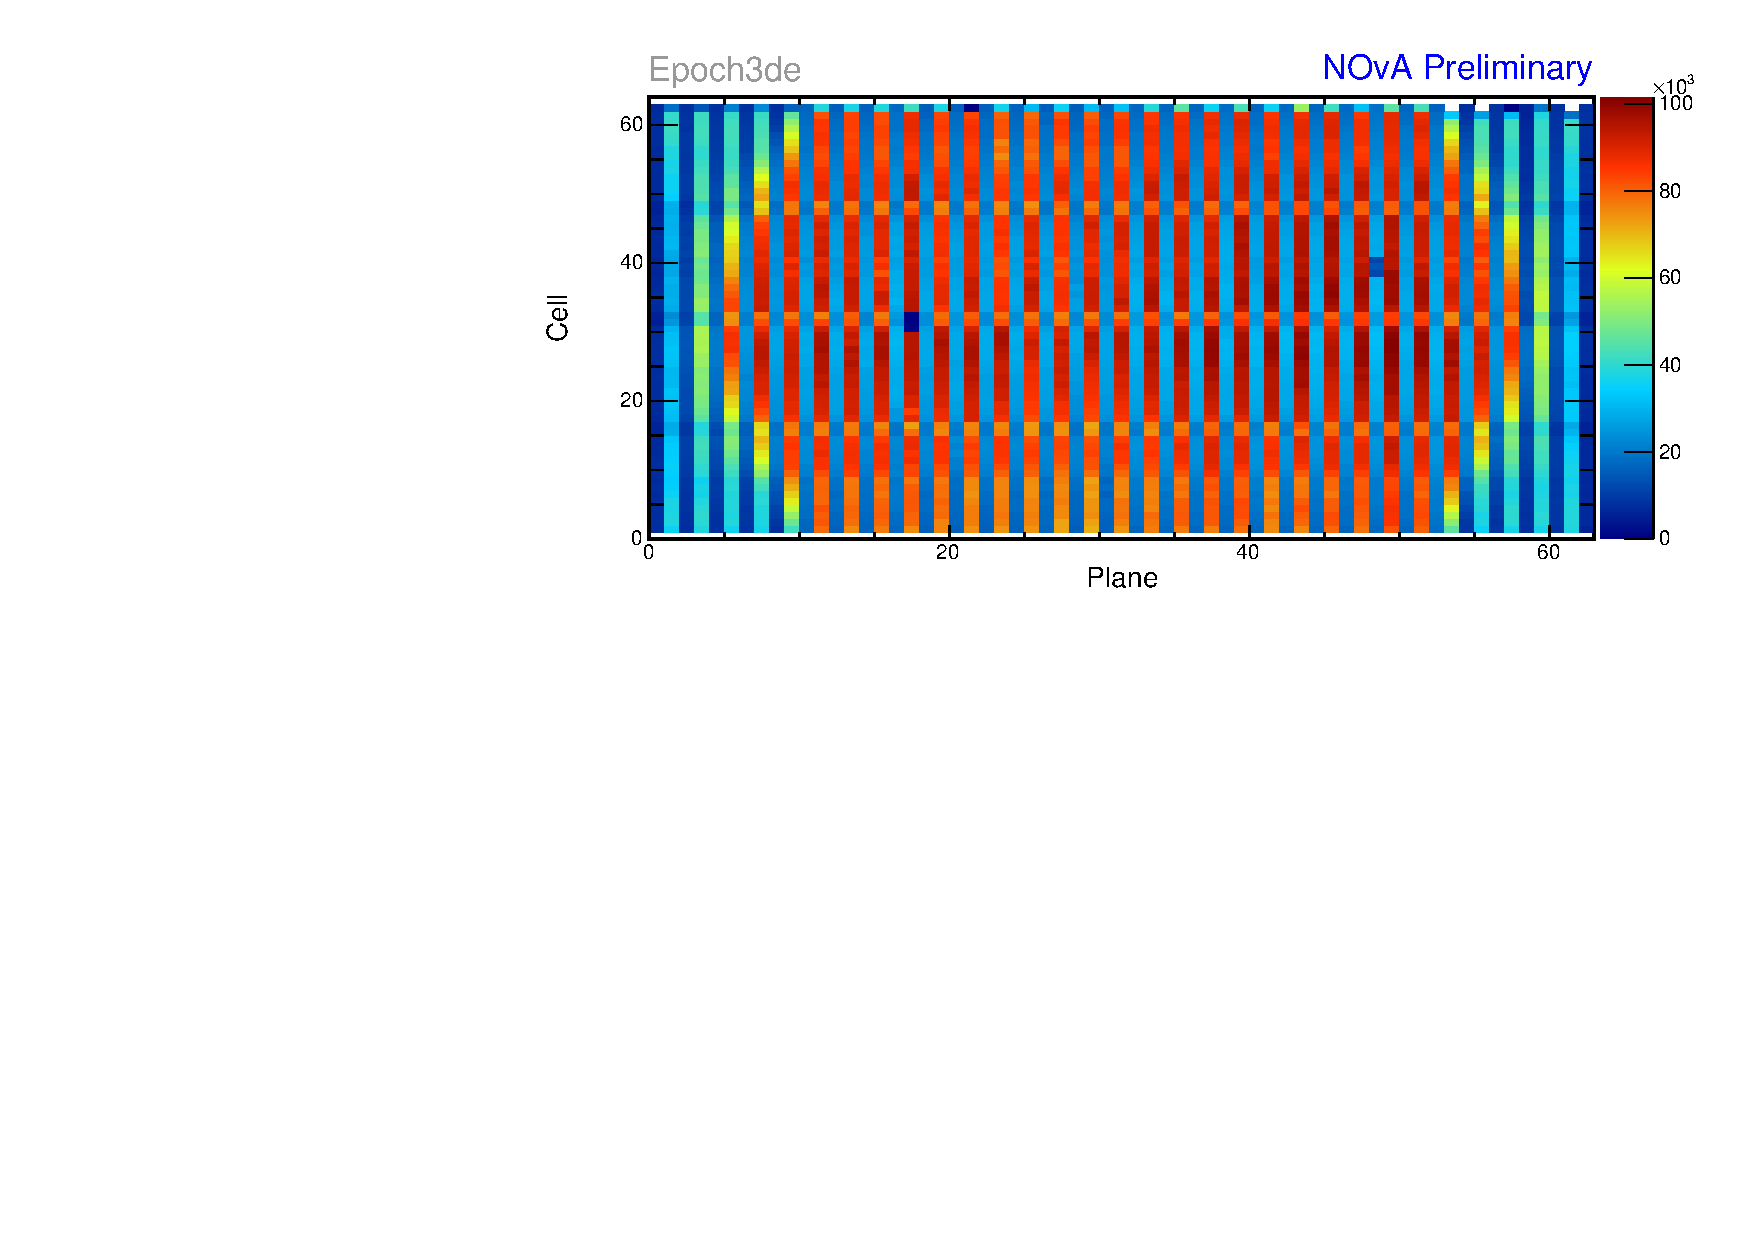
\includegraphics[width=0.9\textwidth]{Plots/Attenprofs_P3Data_CellPlane_Epoch3de.pdf}
\end{subfigure}
\caption{Distribution of events in the period 3, epoch 3a Test Beam data calibration sample.}
\end{figure}

\begin{figure}[!hbtp]
\centering
\begin{subfigure}[b]{0.495\textwidth}
\centering
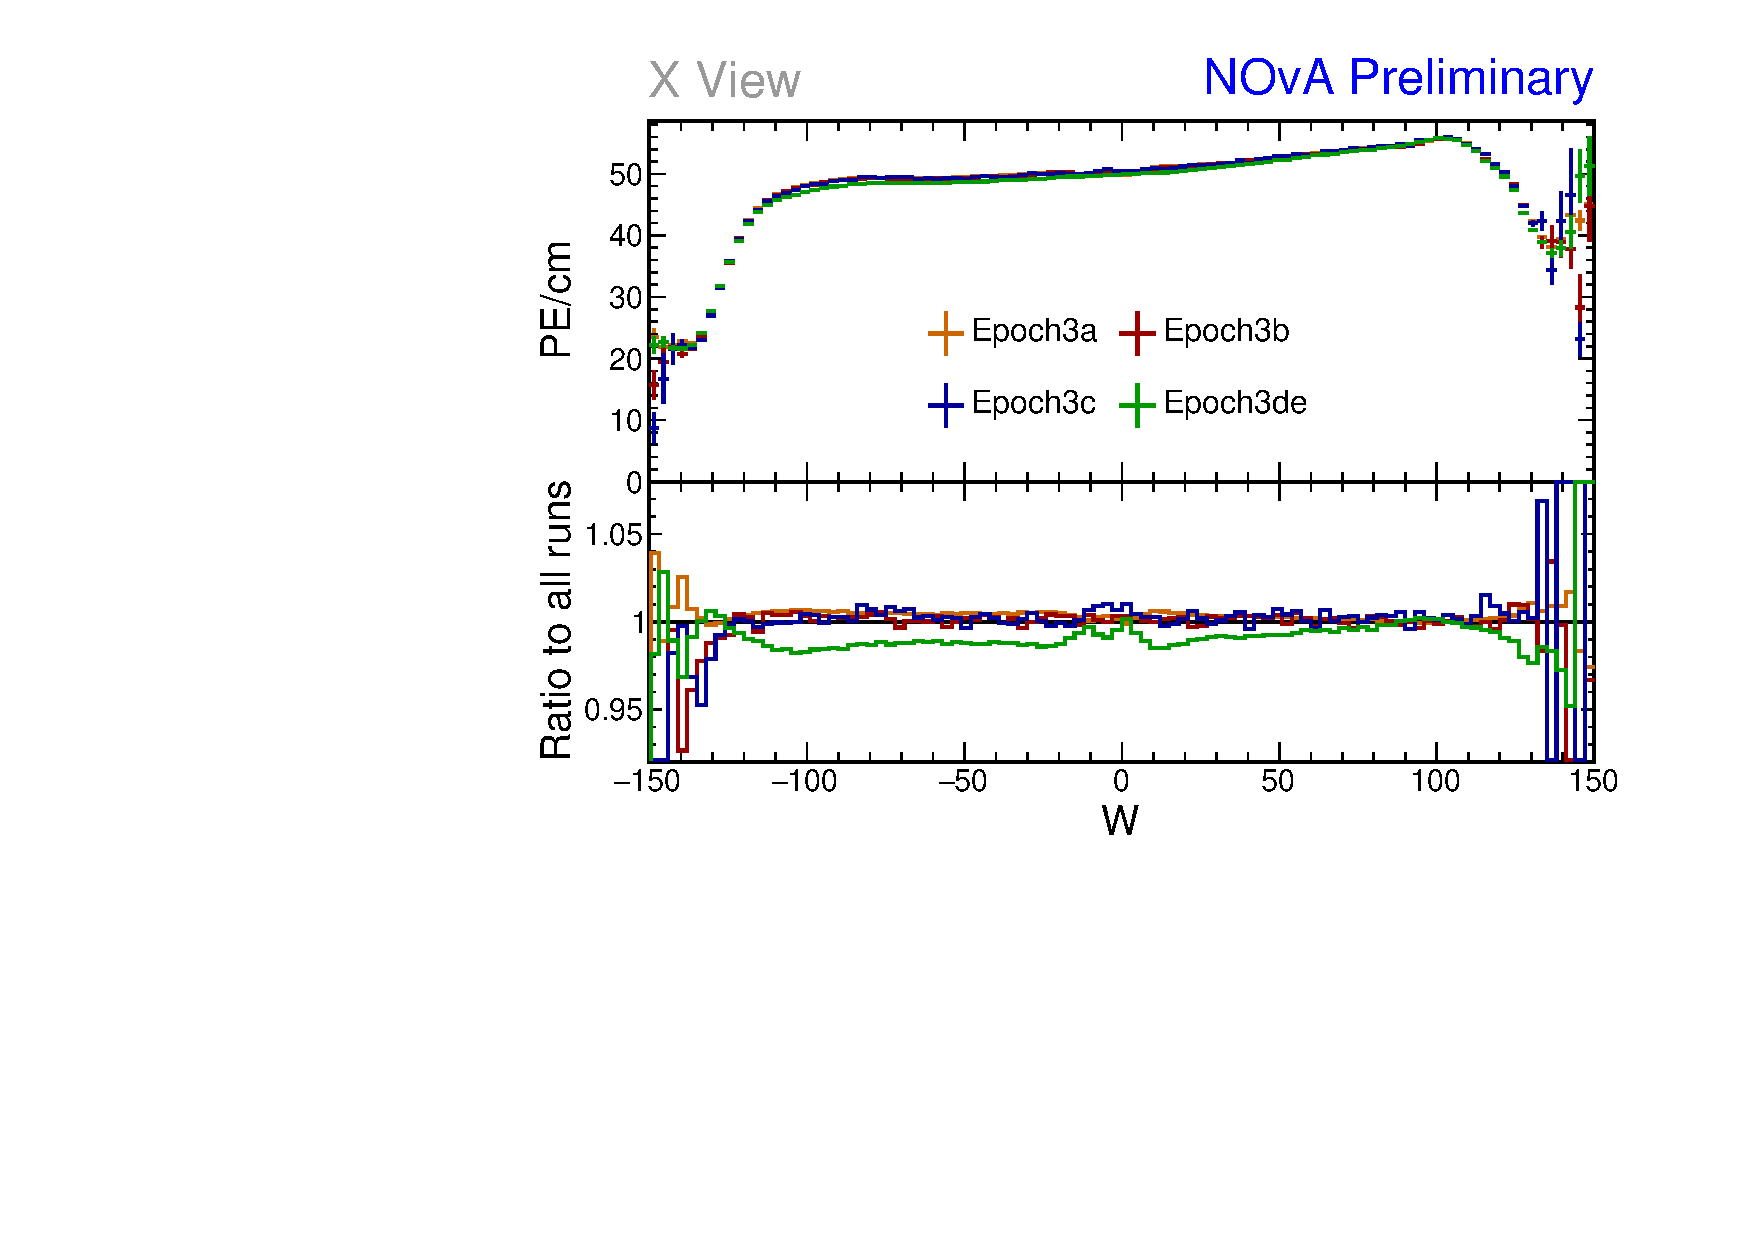
\includegraphics[width=\textwidth]{Plots/Attenprofs_P3Data_WPE_corr_xy_X_Combined.pdf}
\end{subfigure}
\begin{subfigure}[b]{0.495\textwidth}
\centering
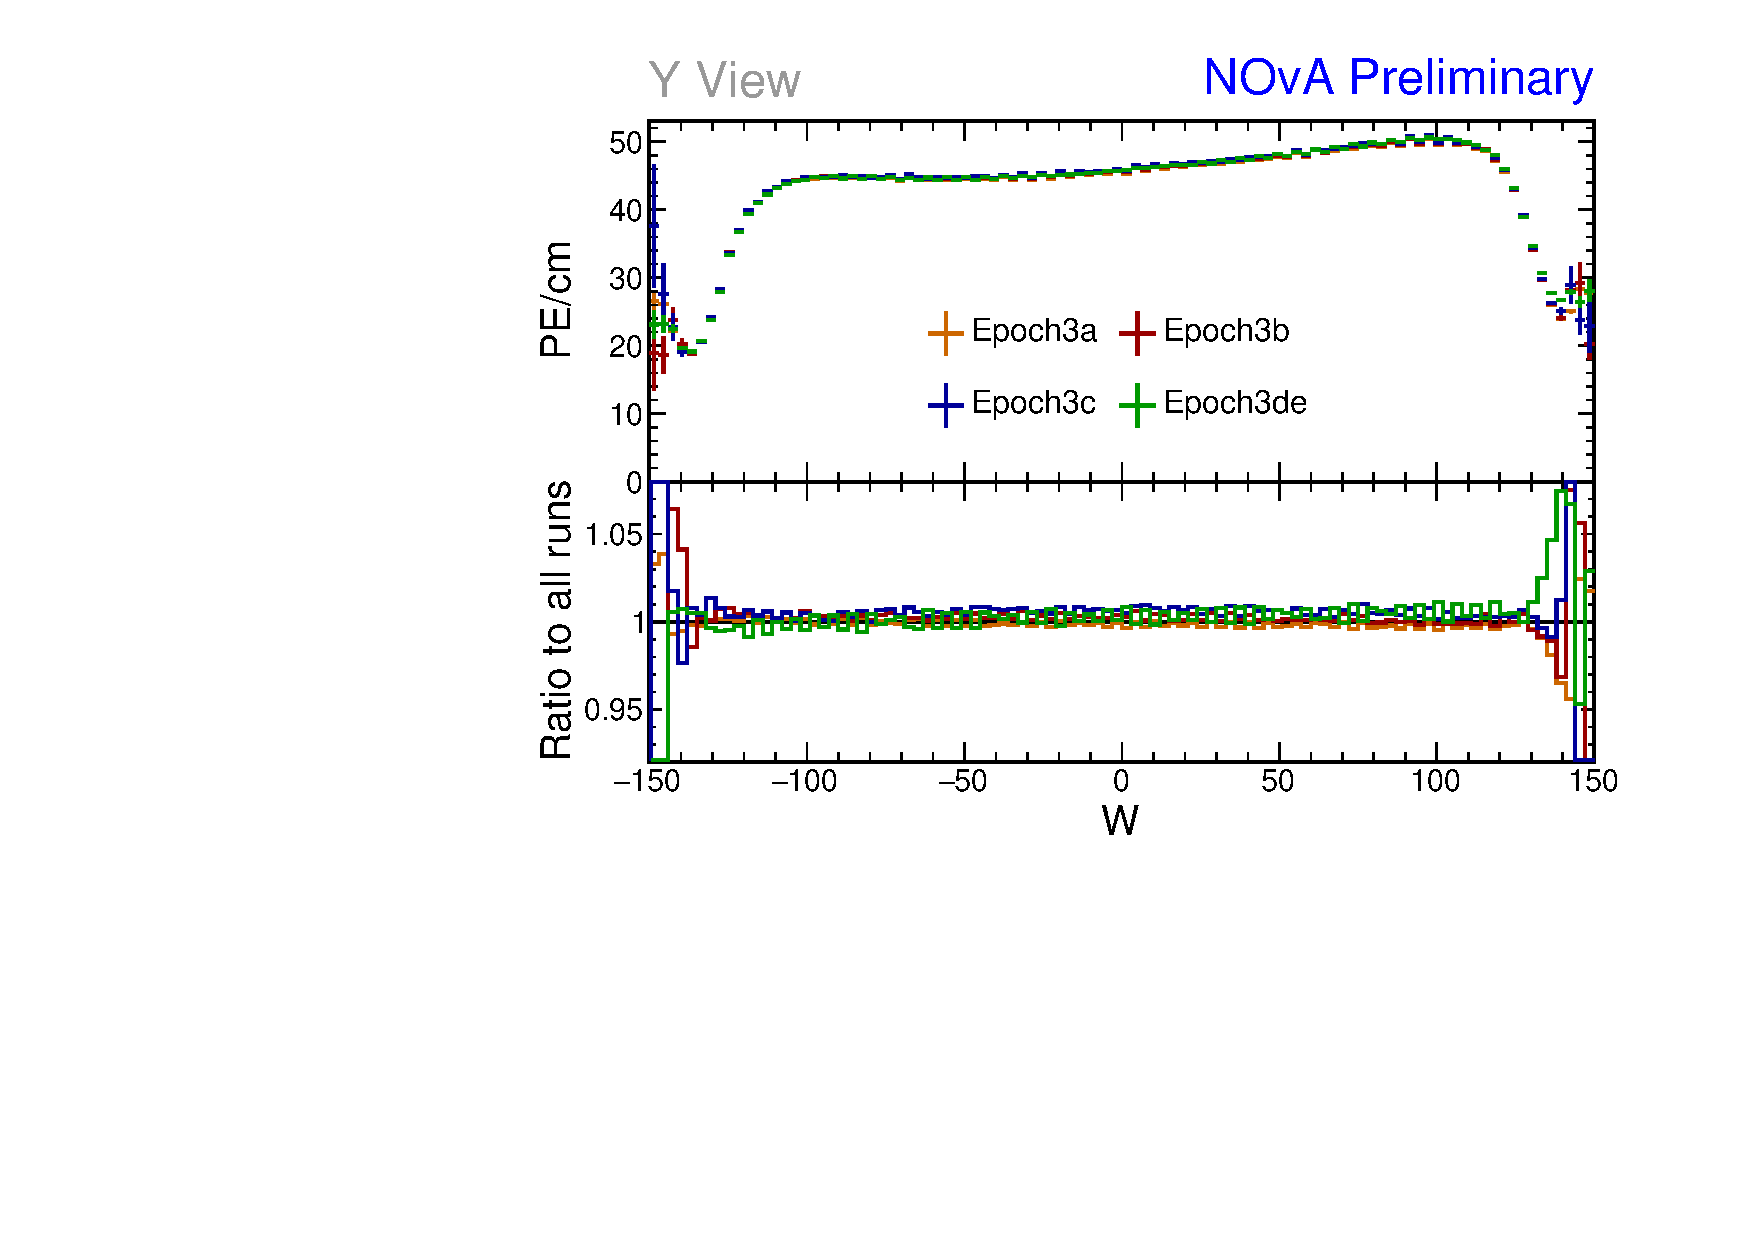
\includegraphics[width=\textwidth]{Plots/Attenprofs_P3Data_WPE_corr_xy_Y_Combined.pdf}
\end{subfigure}
\caption{Uncorrected average energy response as a function of the position within a cell (w) for epochs in period 3.}
\label{figCalibhistWPE_period3}
\end{figure}

\begin{figure}[!hbtp]
\centering
\begin{subfigure}[b]{0.495\textwidth}
\centering
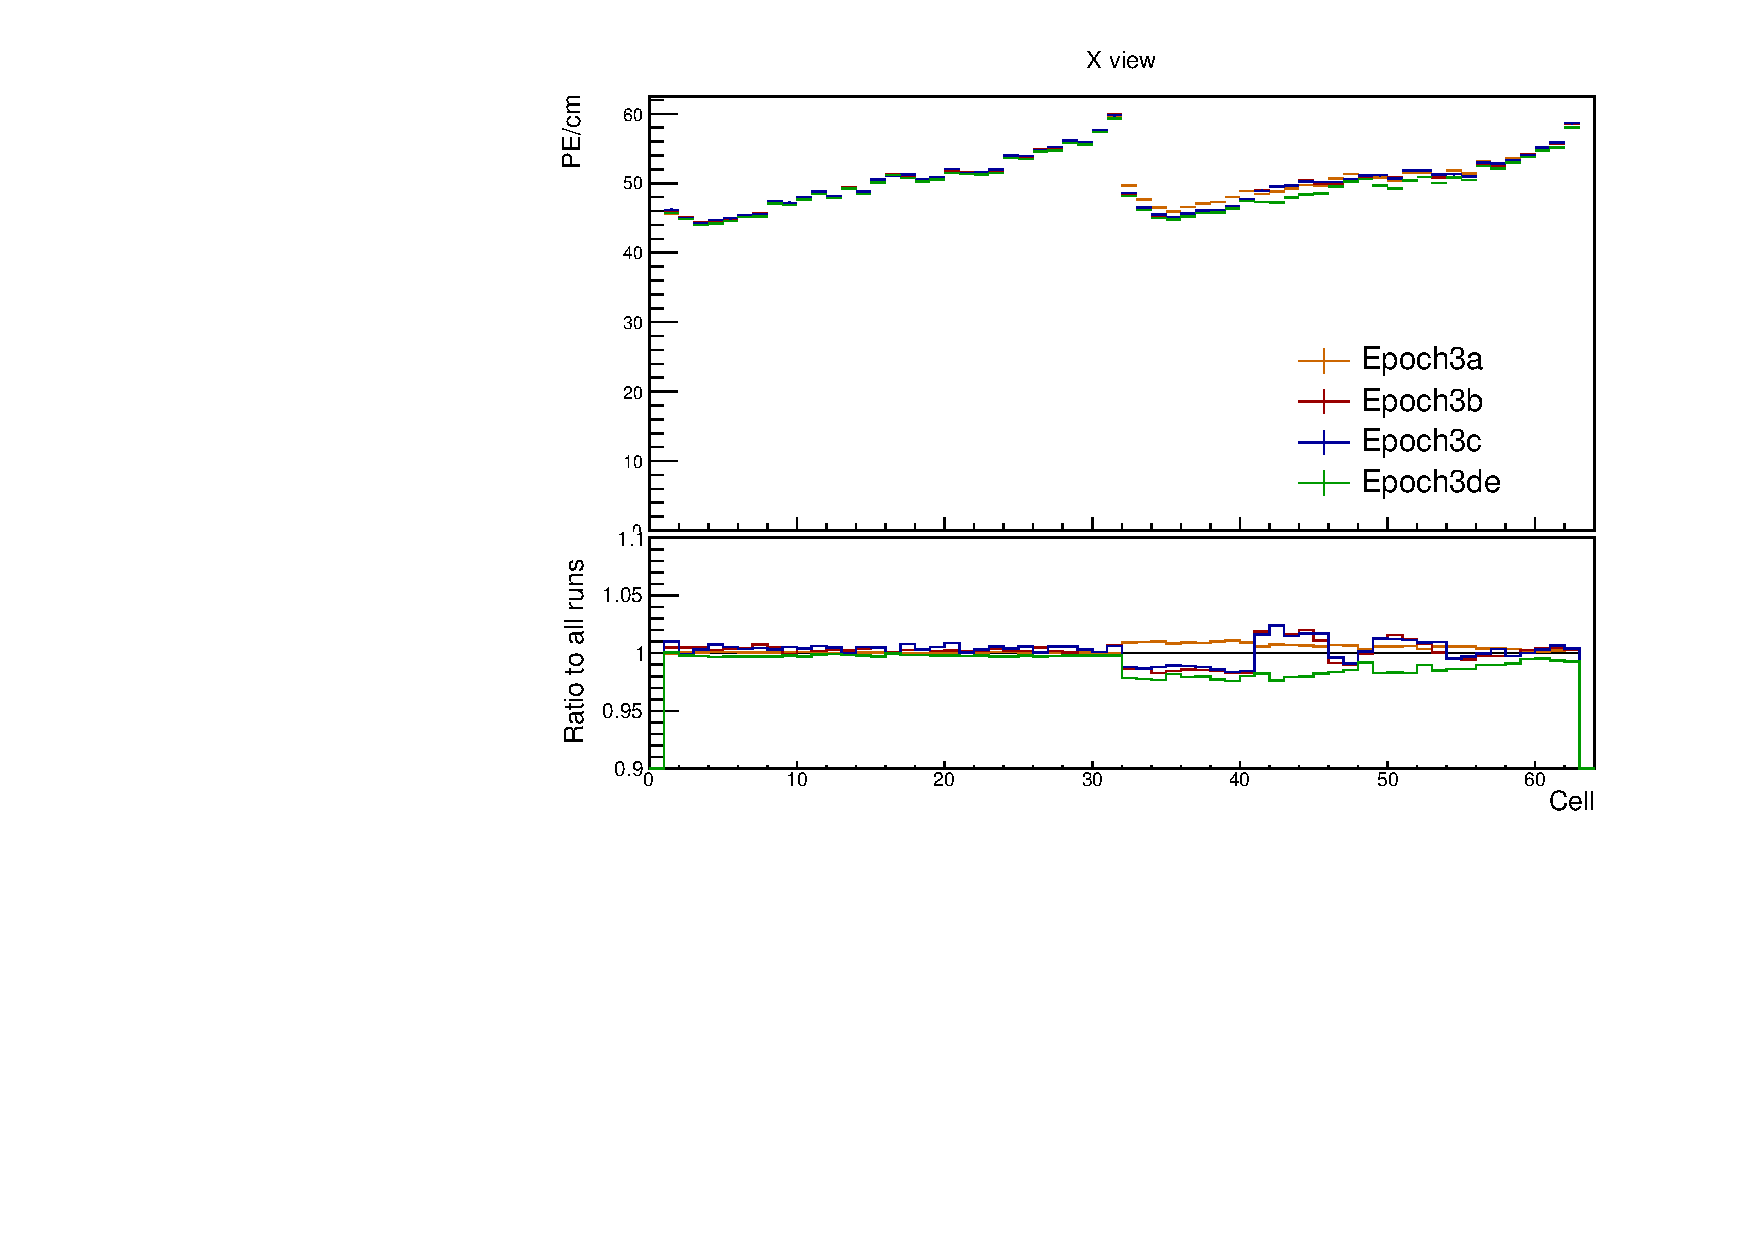
\includegraphics[width=\textwidth]{Plots/Attenprofs_P3Data_CellPE_X_Combined.pdf}
\end{subfigure}
\begin{subfigure}[b]{0.495\textwidth}
\centering
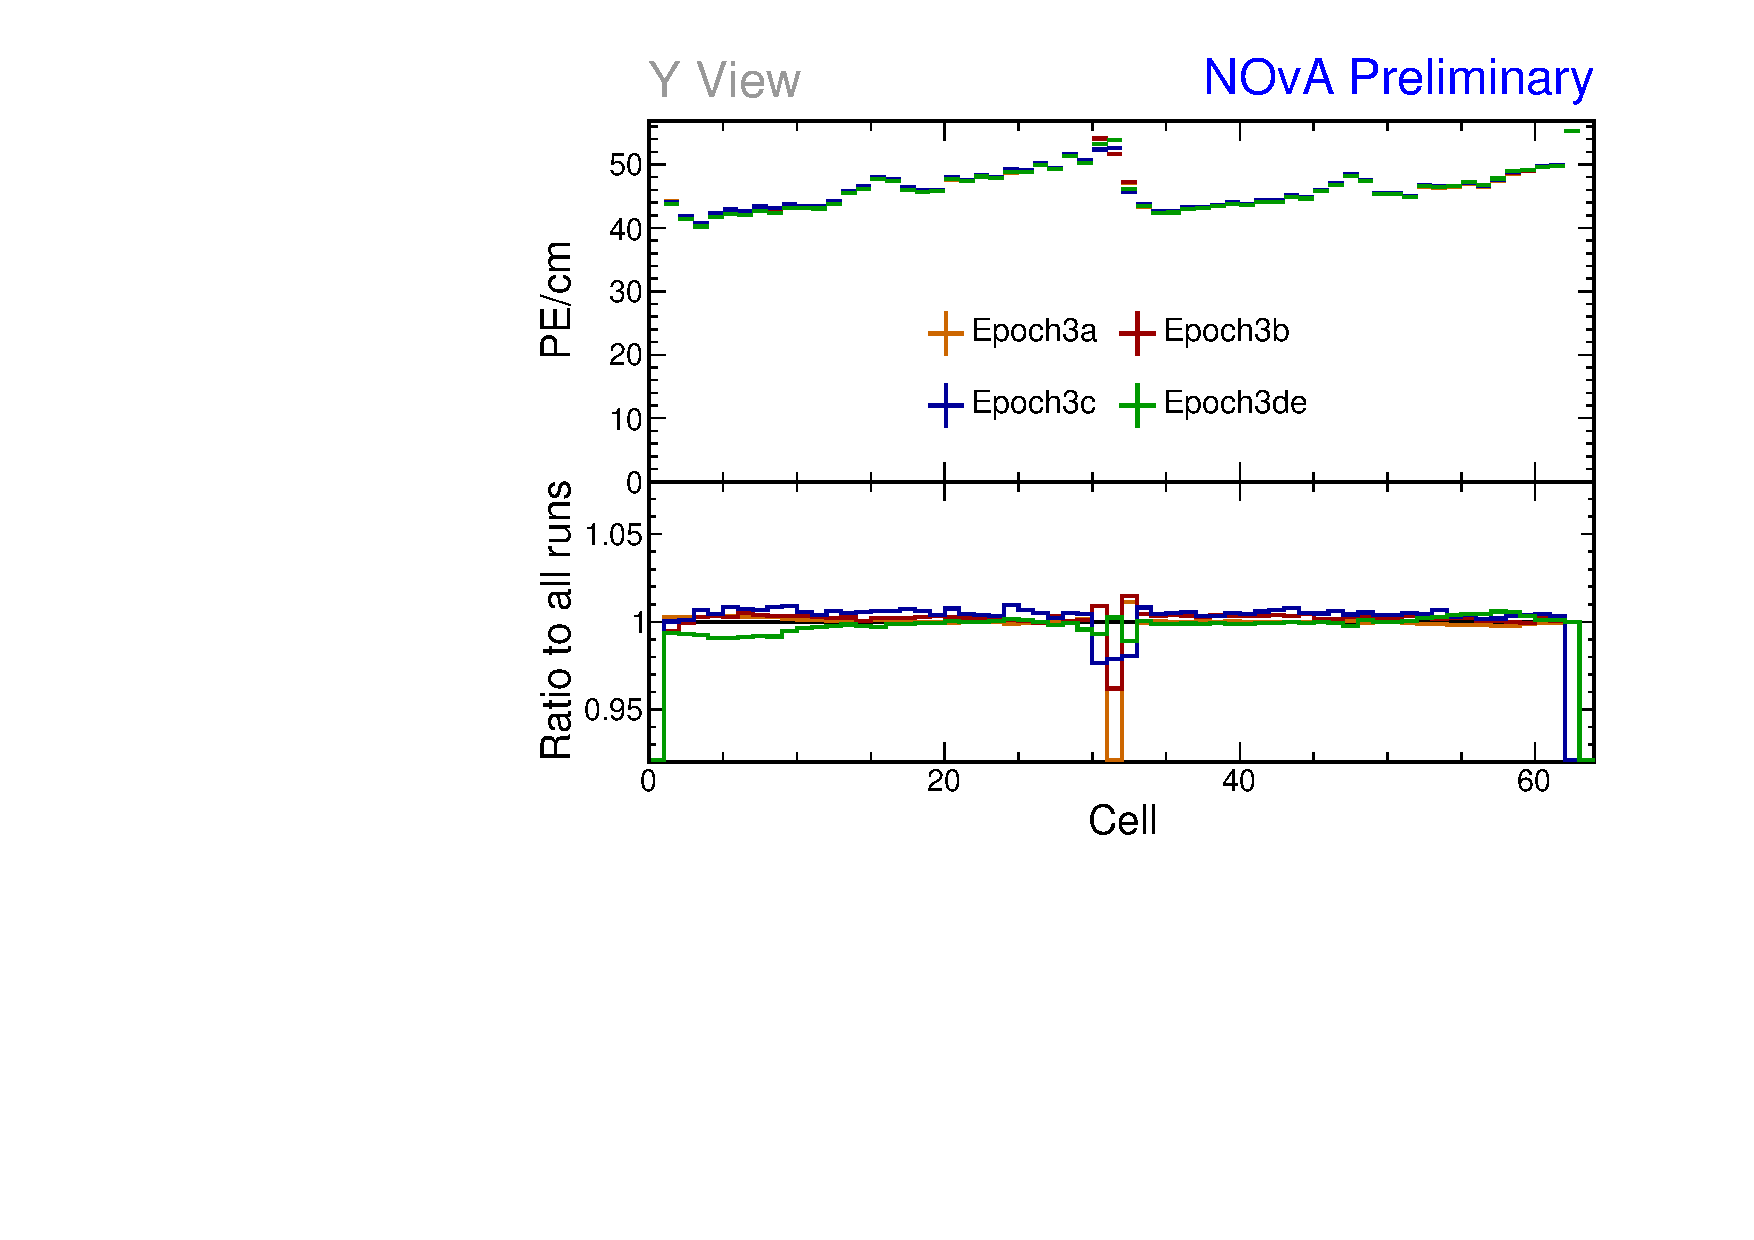
\includegraphics[width=\textwidth]{Plots/Attenprofs_P3Data_CellPE_Y_Combined.pdf}
\end{subfigure}
\caption{Uncorrected average energy response as a function of cells for epochs in period 3.}
\label{figCalibhistCellPE_period3}
\end{figure}

\begin{figure}[!hbtp]
\centering
\begin{subfigure}[b]{0.495\textwidth}
\centering
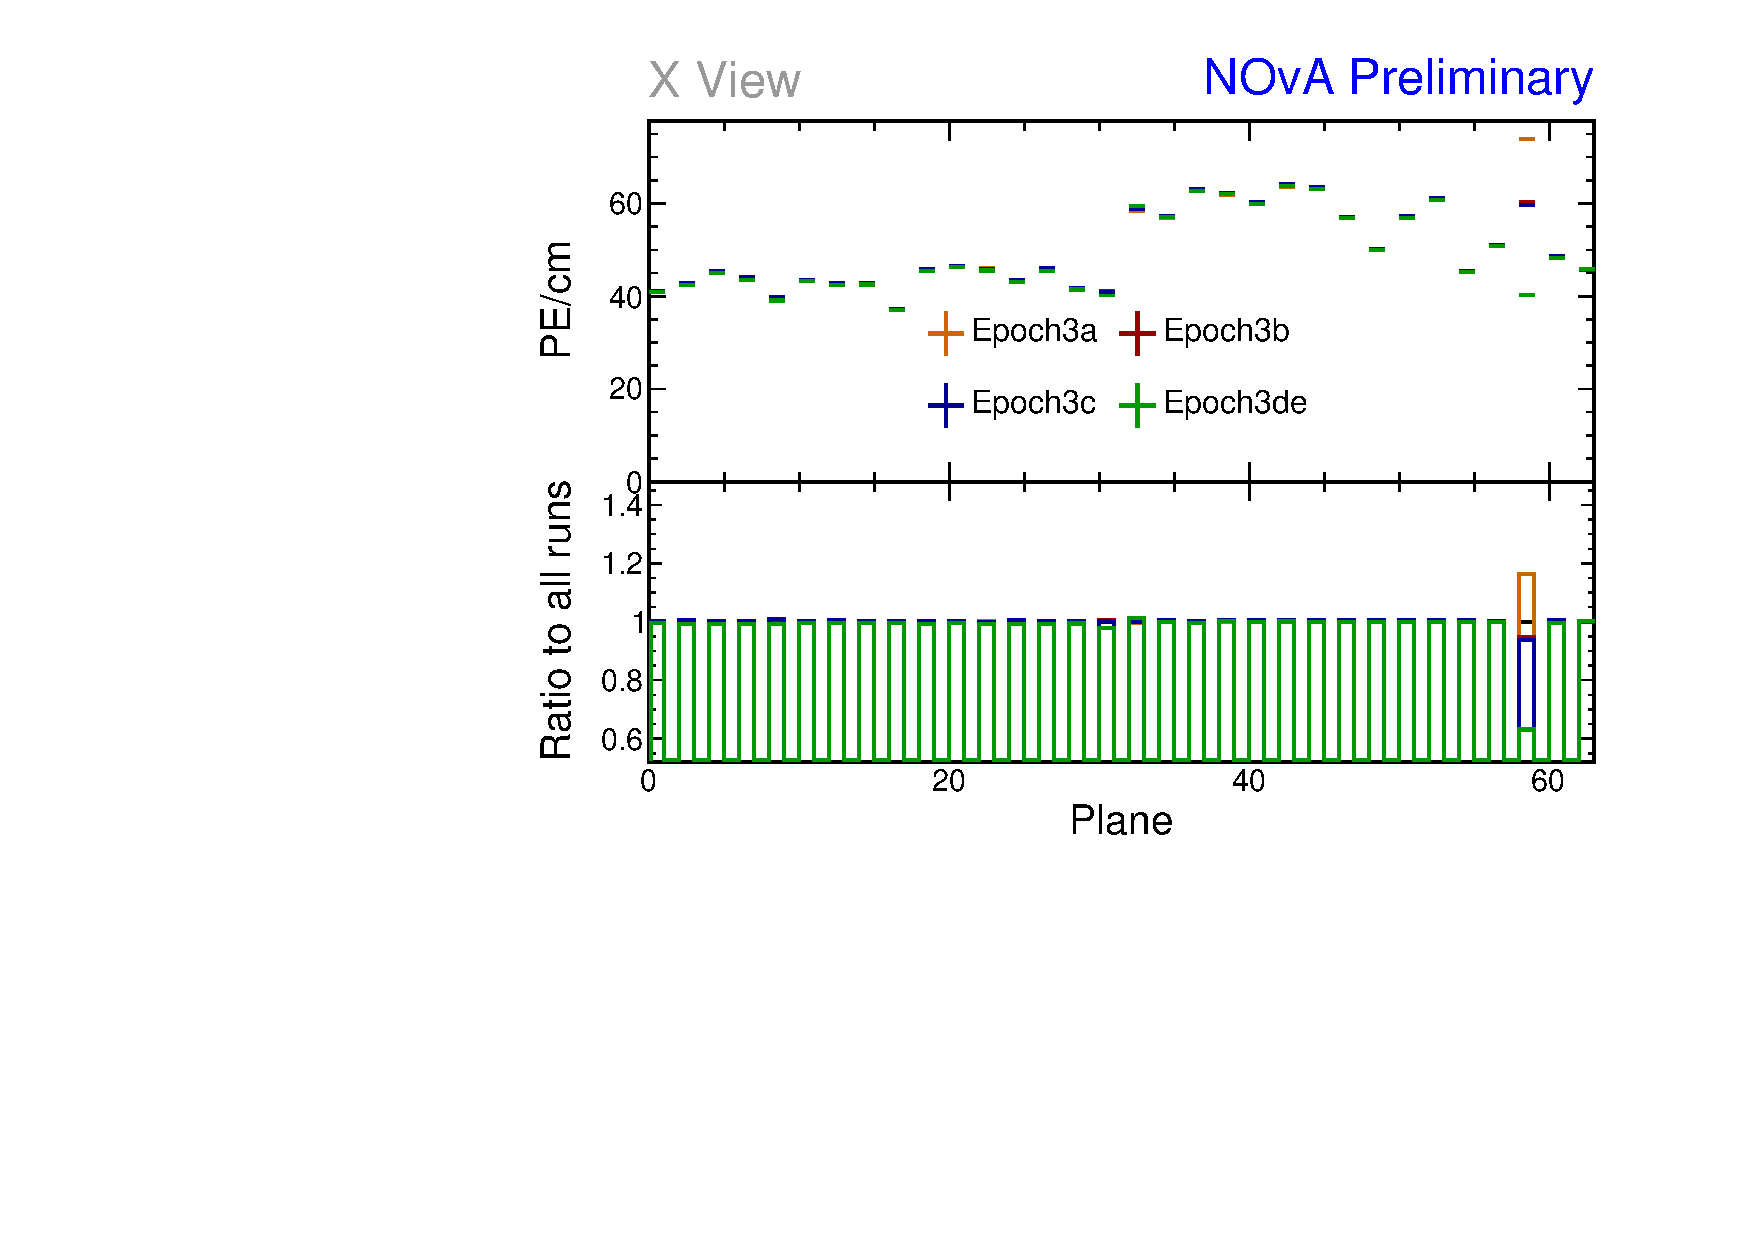
\includegraphics[width=\textwidth]{Plots/Attenprofs_P3Data_PlanePE_X_Combined.pdf}
\end{subfigure}
\begin{subfigure}[b]{0.495\textwidth}
\centering
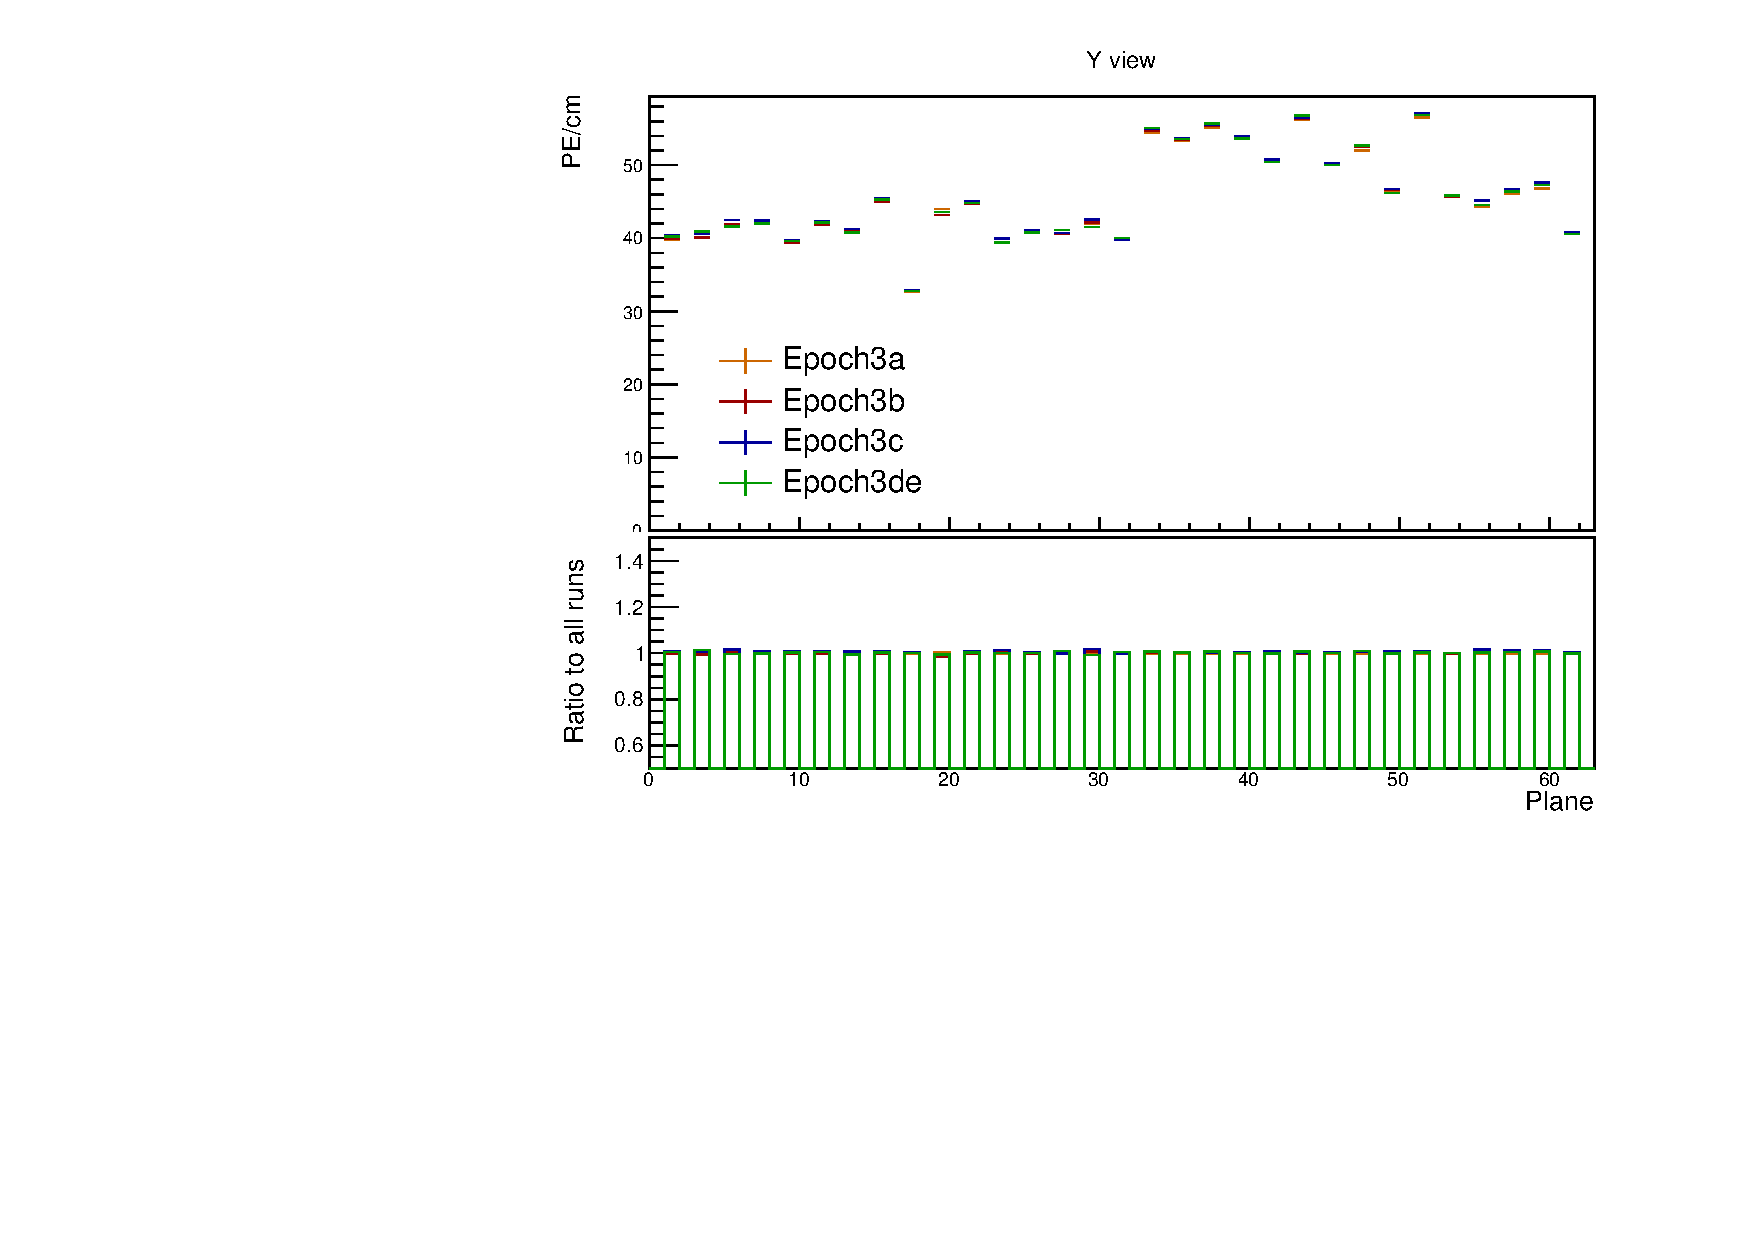
\includegraphics[width=\textwidth]{Plots/Attenprofs_P3Data_PlanePE_Y_Combined.pdf}
\end{subfigure}
\caption{Uncorrected average energy response as a function of planes for epochs in period 3.}
\label{figCalibhistPlanePE_period3}
\end{figure}

\subsubsection{Relative calibration results}

\subsubsection*{Combined epochs 3a, 3b and 3c}

\begin{figure}[!hbtp]
\centering
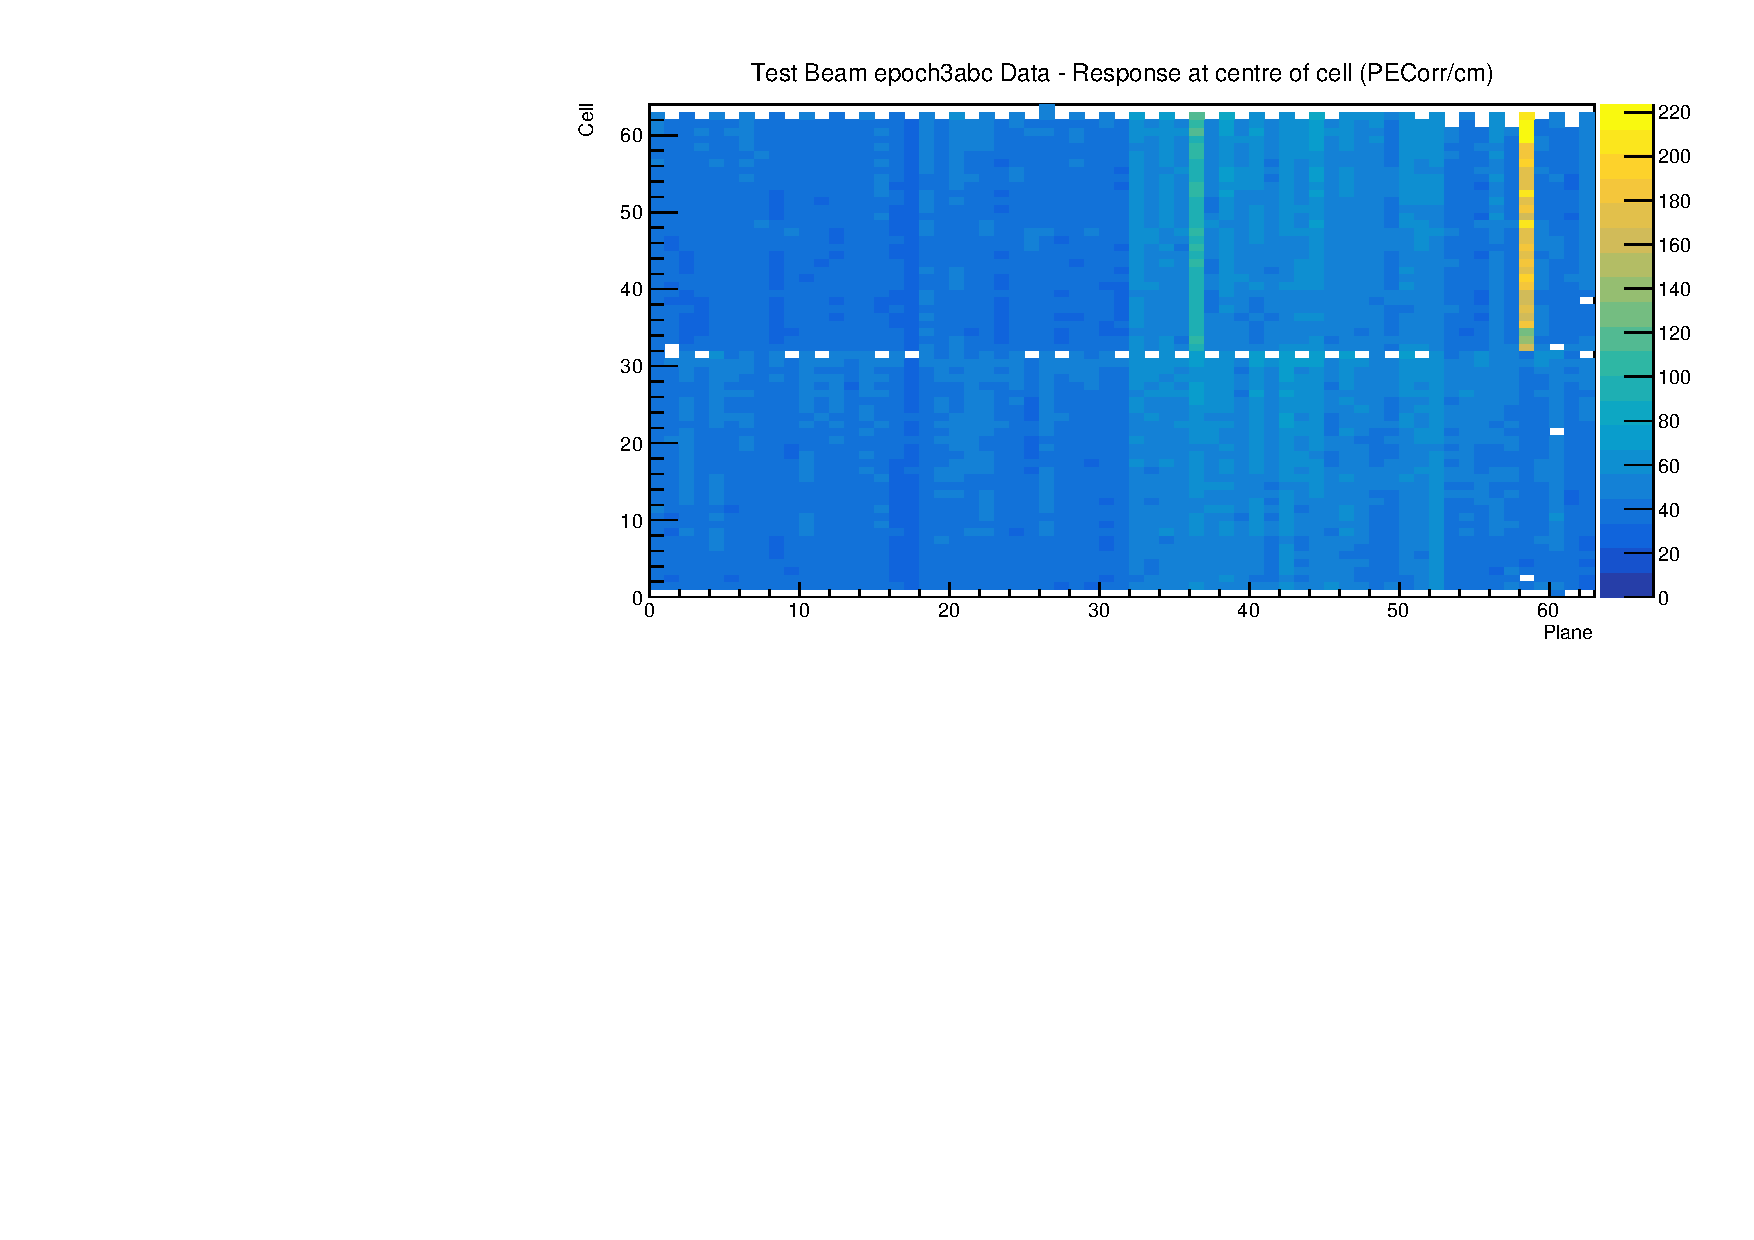
\includegraphics[width=\textwidth]{Plots/CellResponseAtCentre_epoch3abc.pdf}
\caption{Overview of the relative calibration results for the Teast Beam detector period 3, combined epochs 3a, 3b and 3c data. Each cell is represents the average corrected energy response (in PECorr/cm) in the centre of each cell. The blank cells are uncalibrated.}
\end{figure}

\subsubsection*{Combined epochs 3d and 3e}

\begin{figure}[!hbtp]
\centering
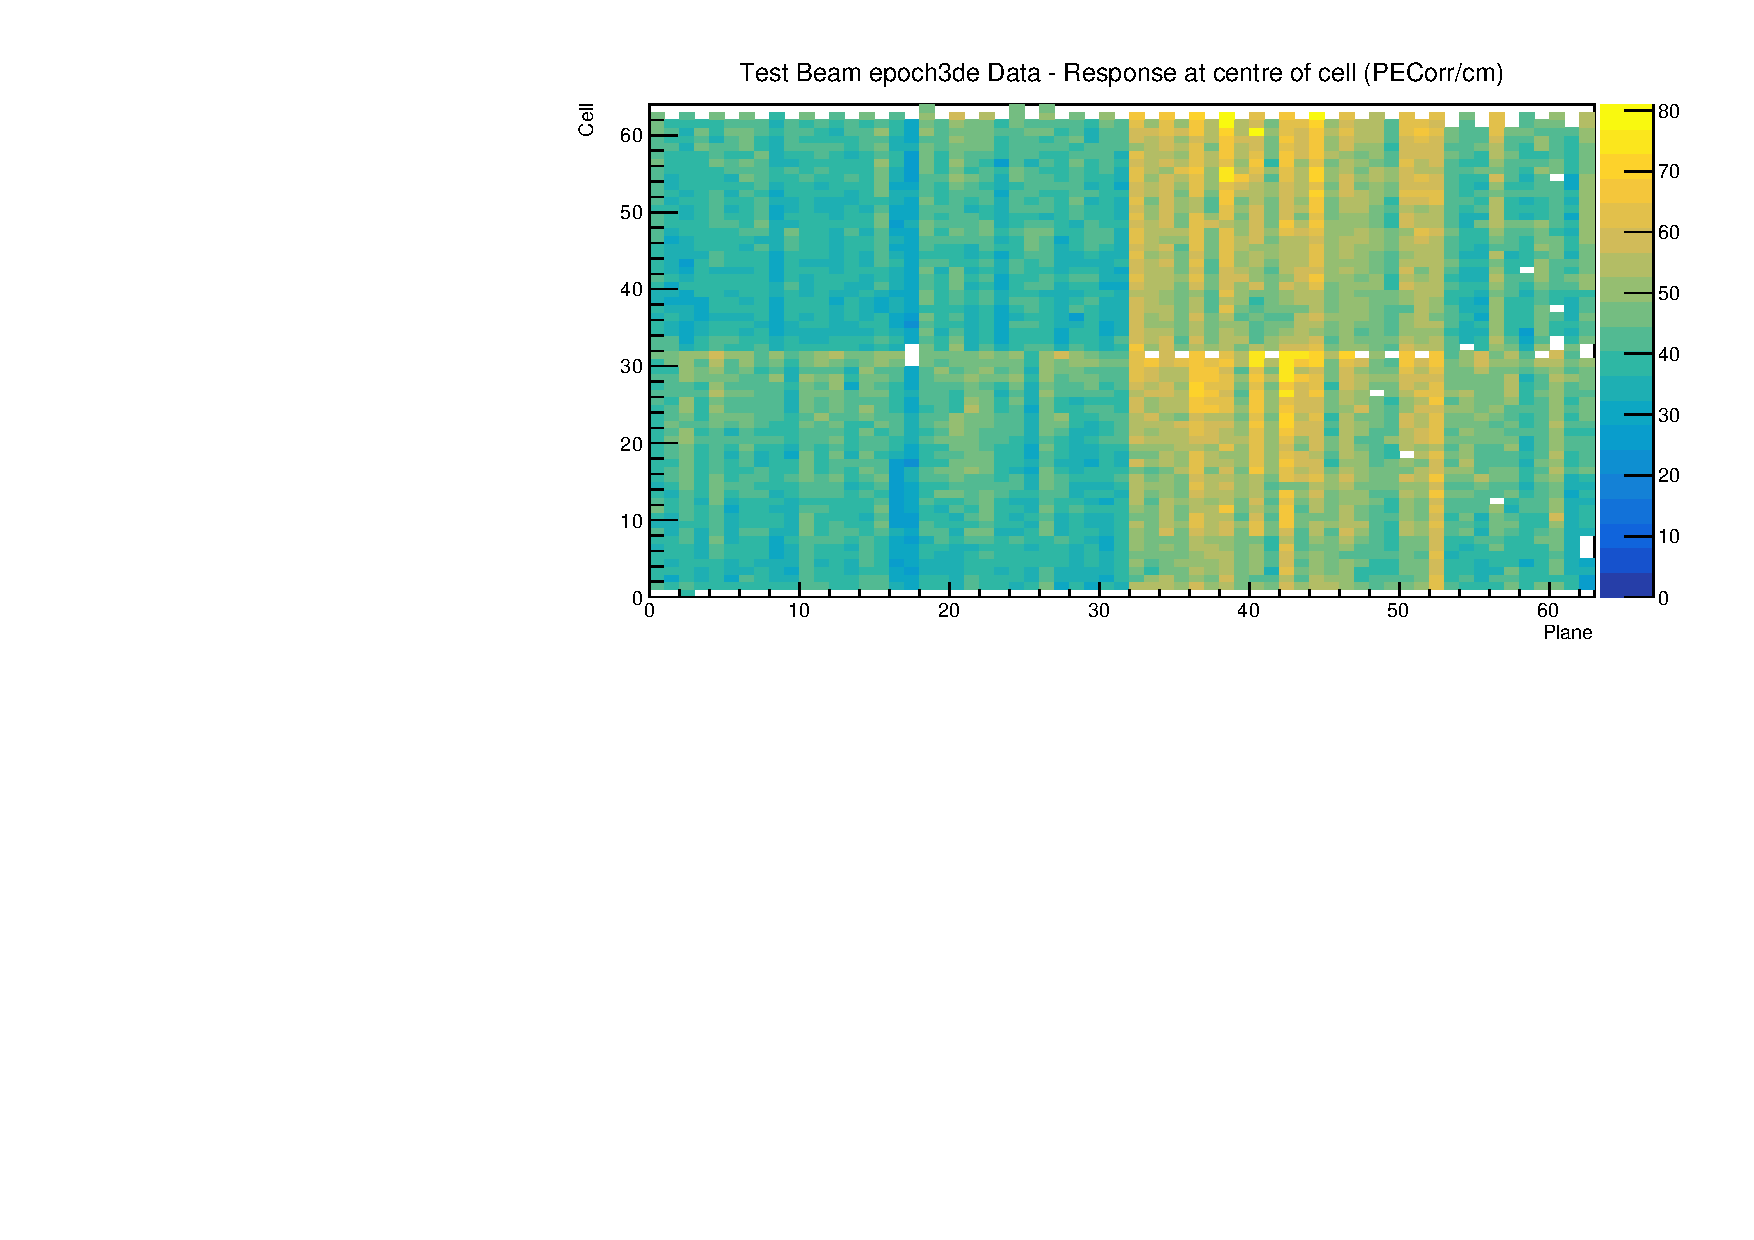
\includegraphics[width=\textwidth]{Plots/CellResponseAtCentre_epoch3de.pdf}
\caption{Overview of the relative calibration results for the Teast Beam detector period 3, combined epochs 3d and 3e data. Each cell is represents the average corrected energy response (in PECorr/cm) in the centre of each cell. The blank cells are uncalibrated.}
\end{figure}

\subsection{Period 4}

\begin{figure}[!hbtp]
\centering
\begin{subfigure}[b]{\textwidth}
\centering
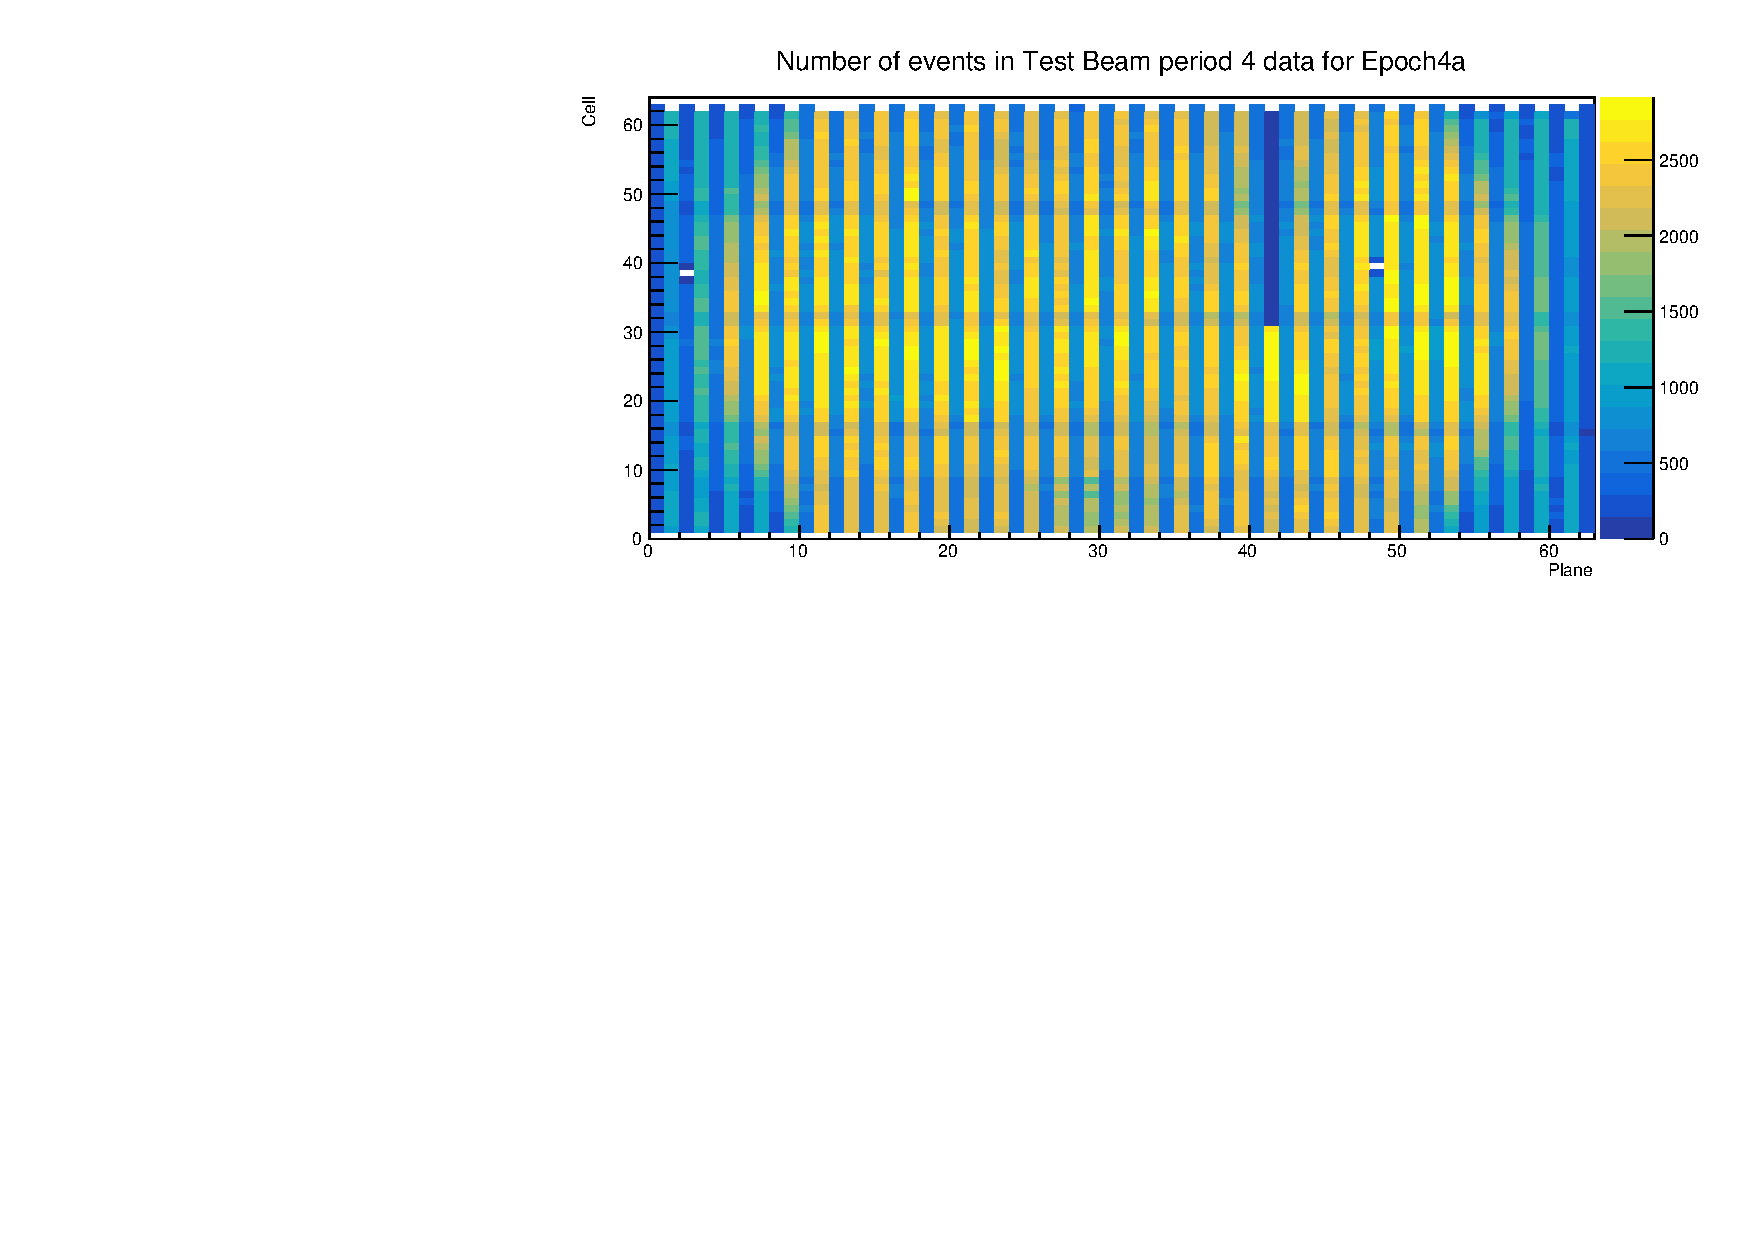
\includegraphics[width=.9\textwidth]{Plots/Attenprofs_P4Data_CellPlane_Epoch4a.pdf}
\end{subfigure}
\begin{subfigure}[b]{\textwidth}
\centering
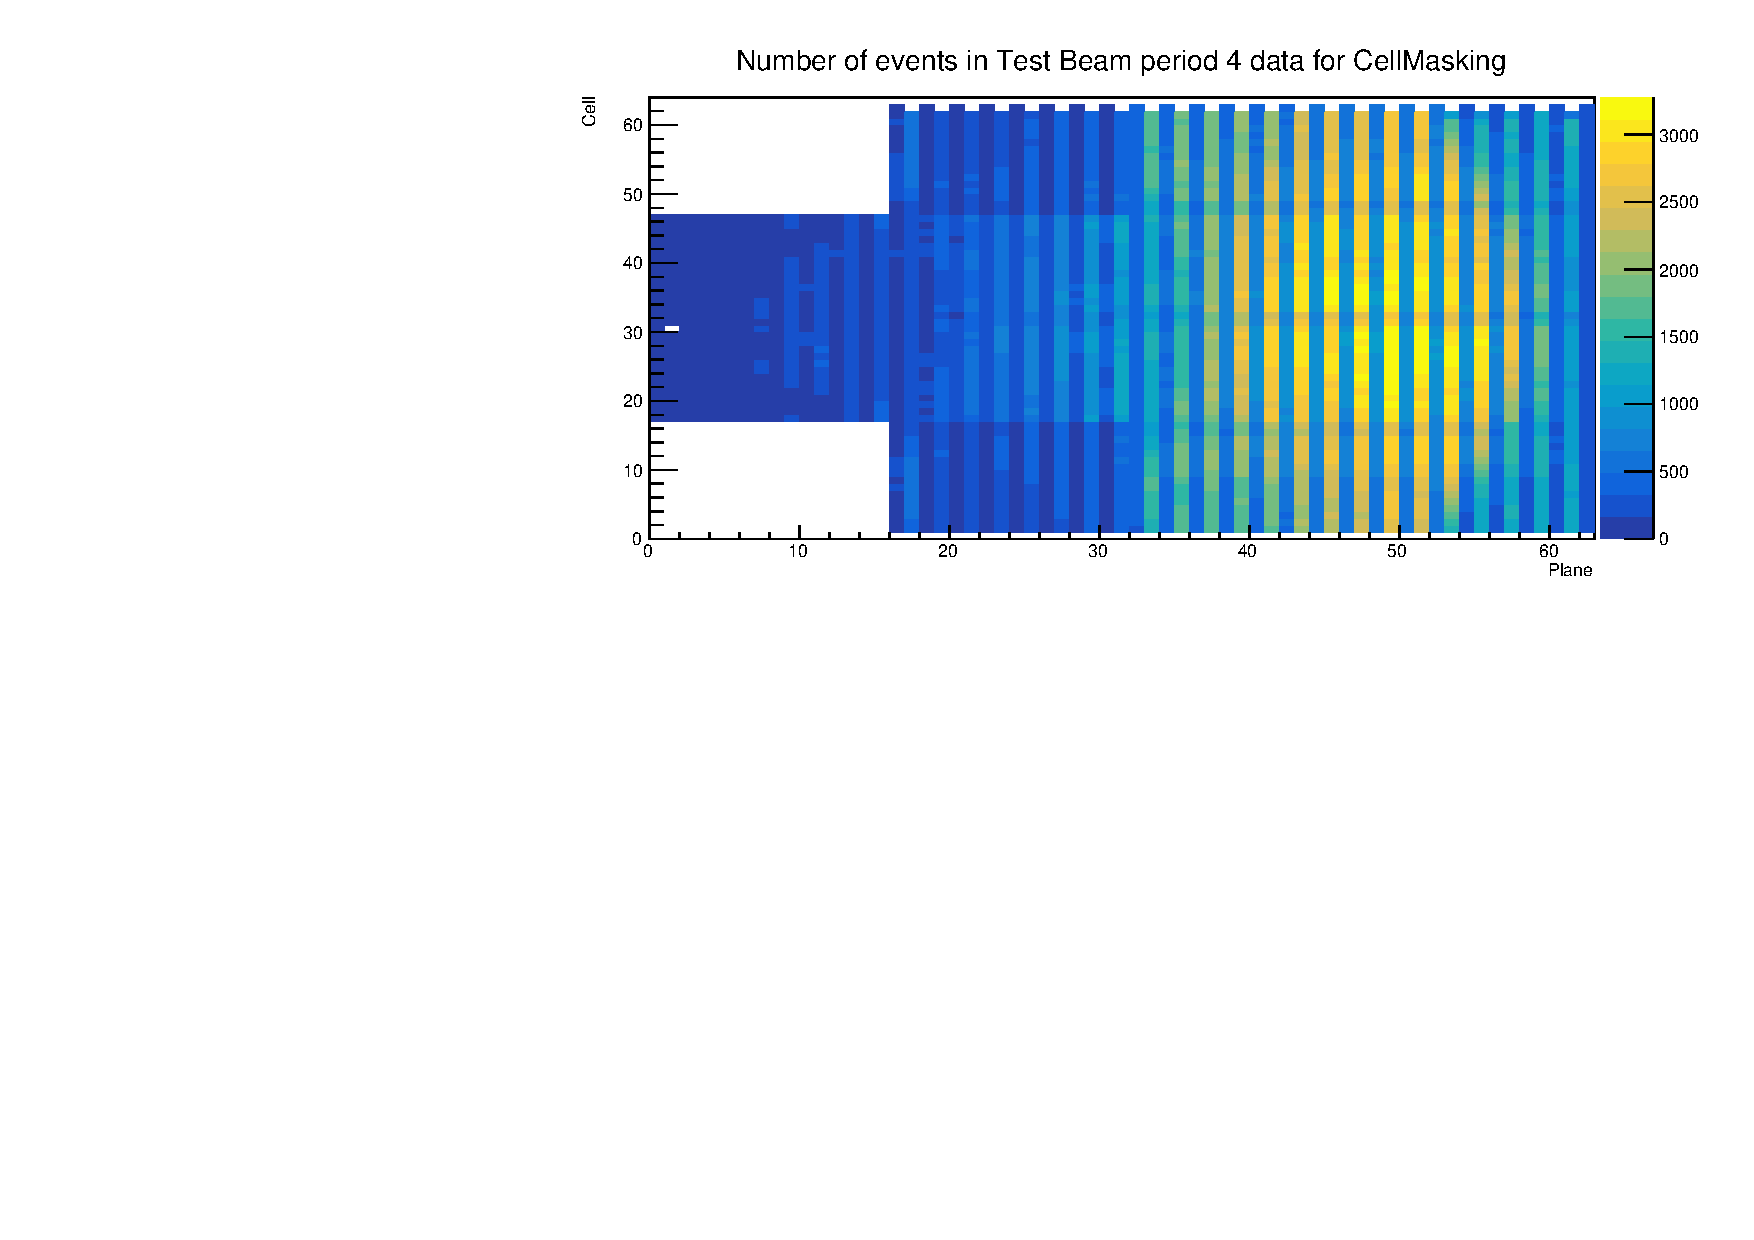
\includegraphics[width=.9\textwidth]{Plots/Attenprofs_P4Data_CellPlane_CellMasking.pdf}
\end{subfigure}
\begin{subfigure}[b]{\textwidth}
\centering
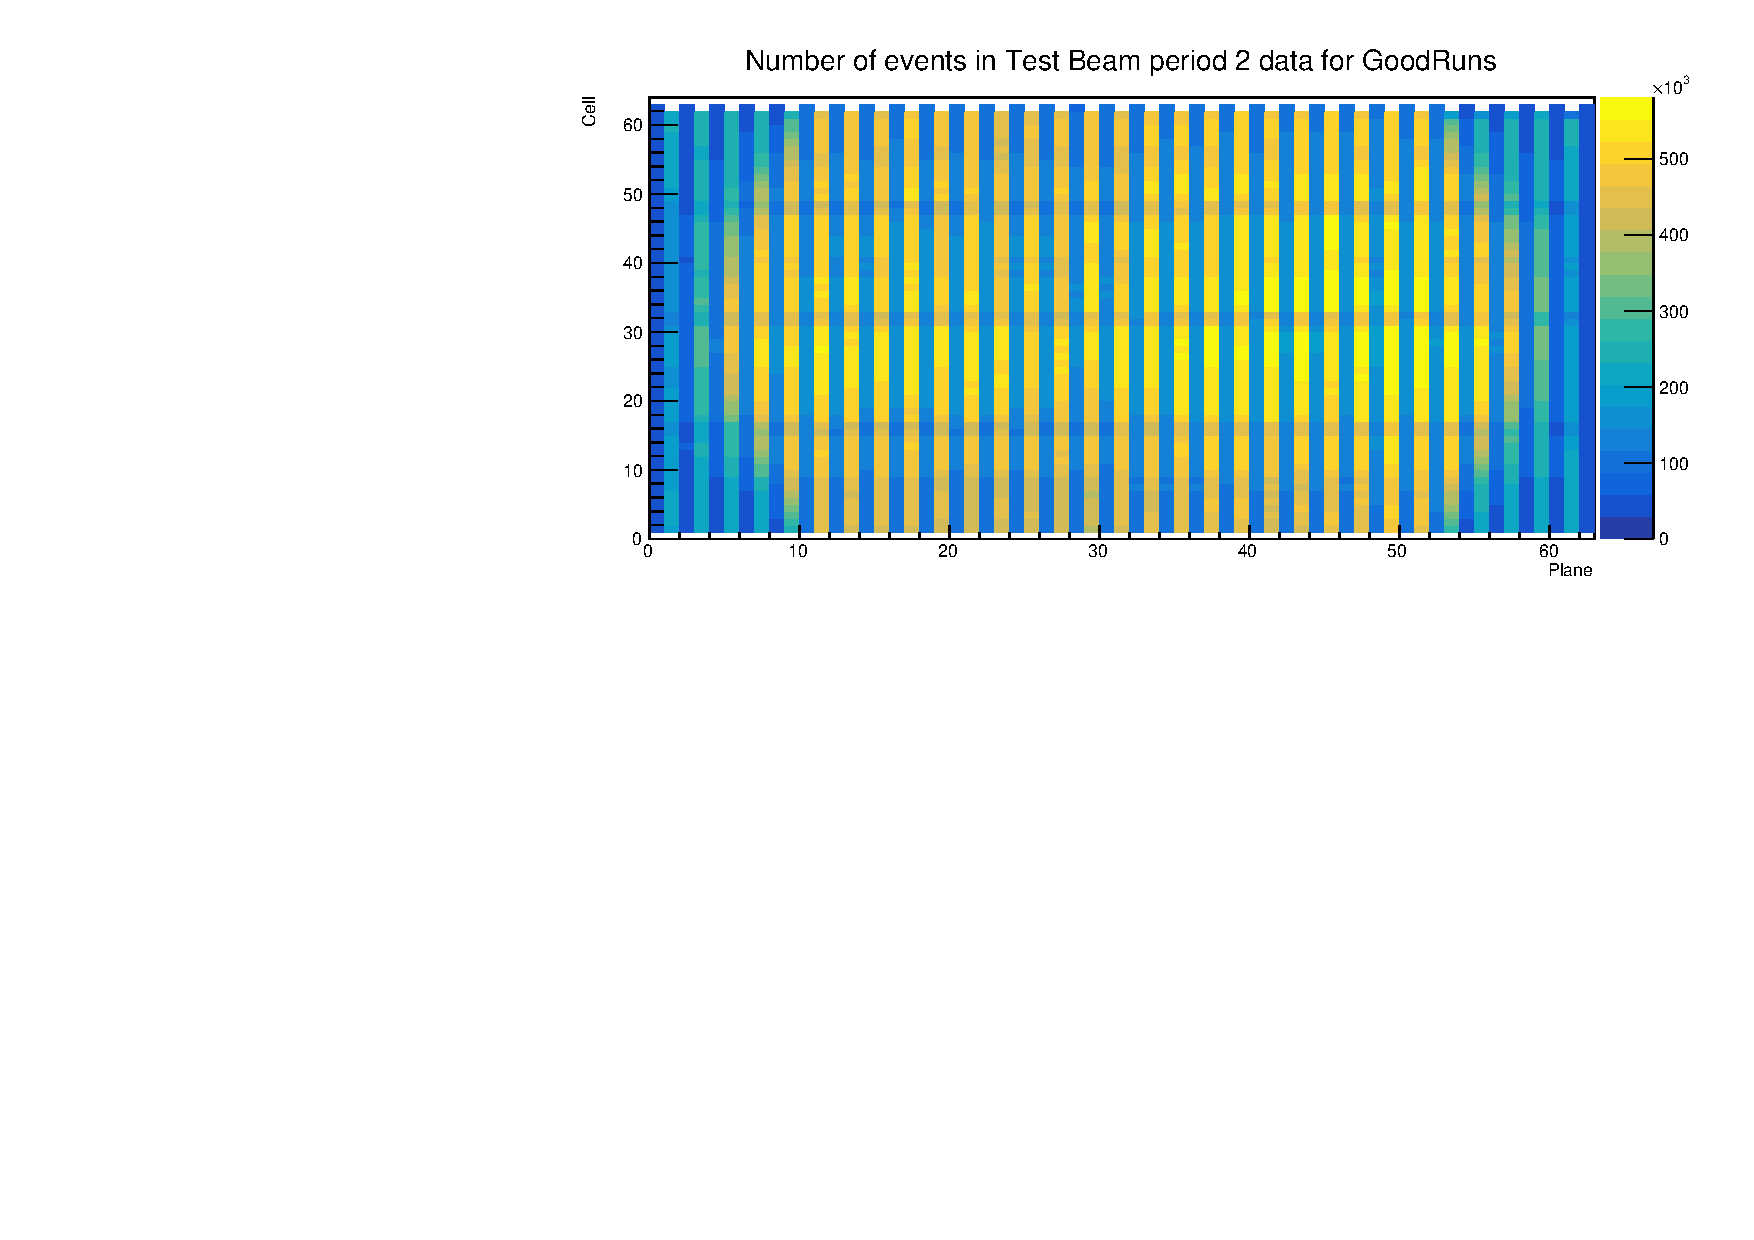
\includegraphics[width=.9\textwidth]{Plots/Attenprofs_P4Data_CellPlane_GoodRuns.pdf}
\end{subfigure}
\caption{Distribution of events in the Test Beam period 4 data calibration sample. The top plot shows the first three comissioning runs, the middle plot the status of the detector during the Cell Masking studies and the bottom plot shows the rest.}
\end{figure}

\begin{figure}[!hbtp]
\centering
\begin{subfigure}[b]{0.495\textwidth}
\centering
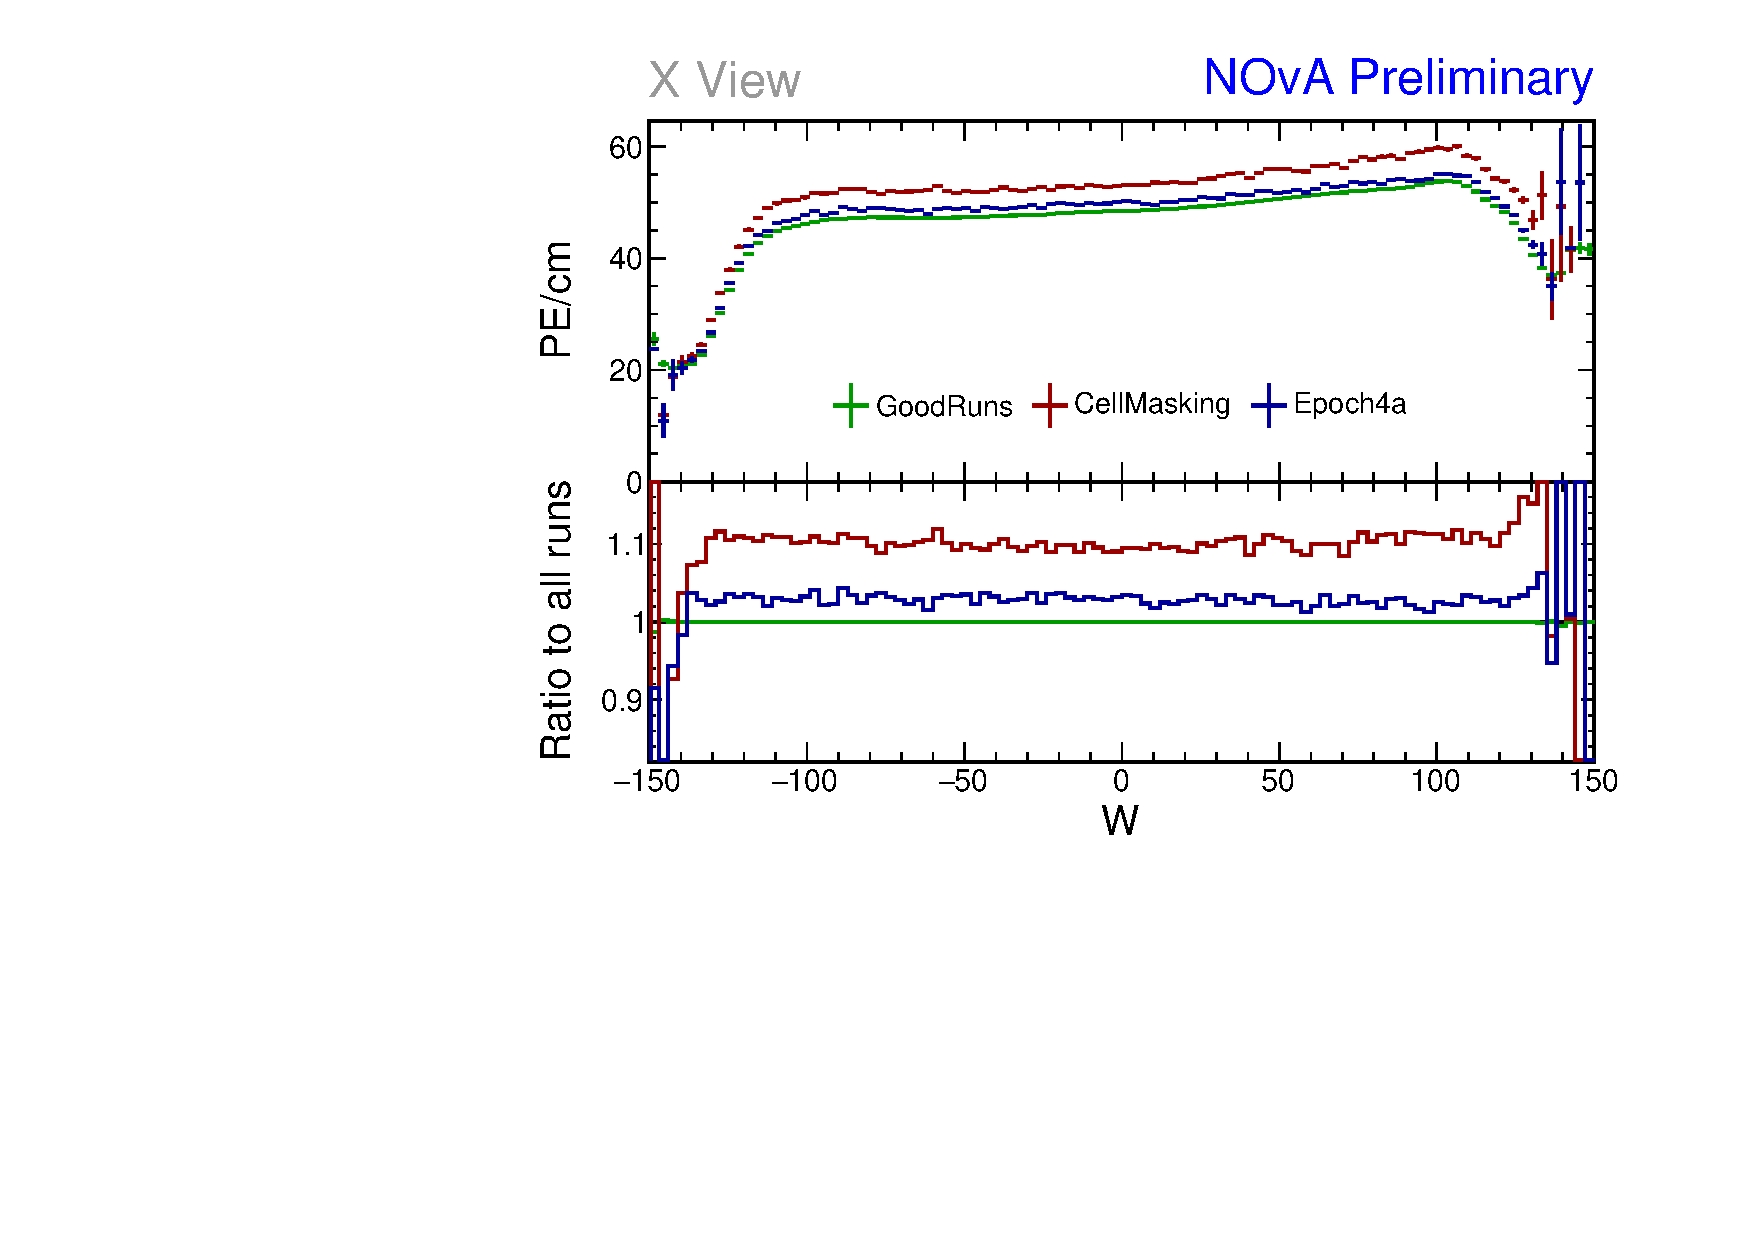
\includegraphics[width=\textwidth]{Plots/Attenprofs_P4Data_WPE_corr_xy_X_Combined.pdf}
\end{subfigure}
\begin{subfigure}[b]{0.495\textwidth}
\centering
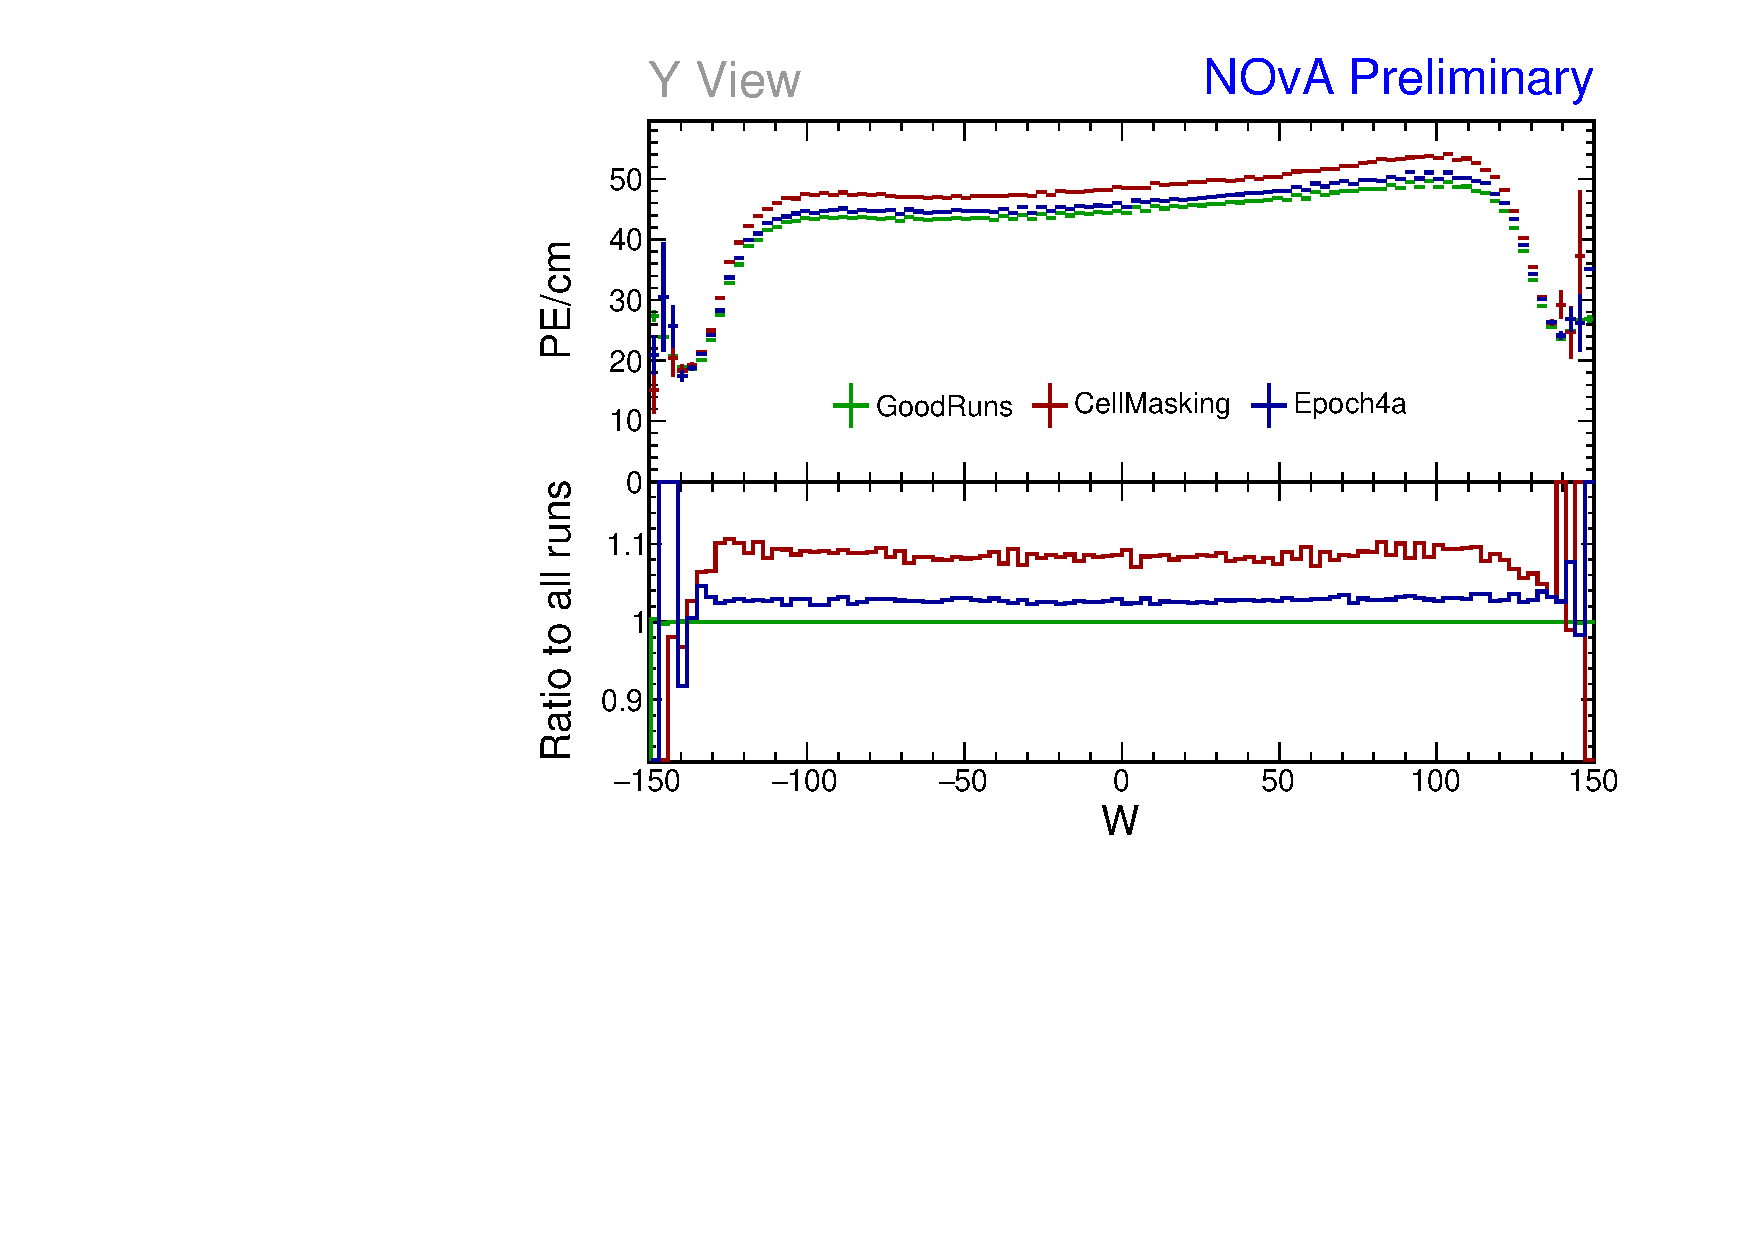
\includegraphics[width=\textwidth]{Plots/Attenprofs_P4Data_WPE_corr_xy_Y_Combined.pdf}
\end{subfigure}
\caption{Uncorrected average energy response as a function of the position within a cell (w) for epochs in period 4.}
\label{figCalibhistWPE_period4}
\end{figure}

\begin{figure}[!hbtp]
\centering
\begin{subfigure}[b]{0.495\textwidth}
\centering
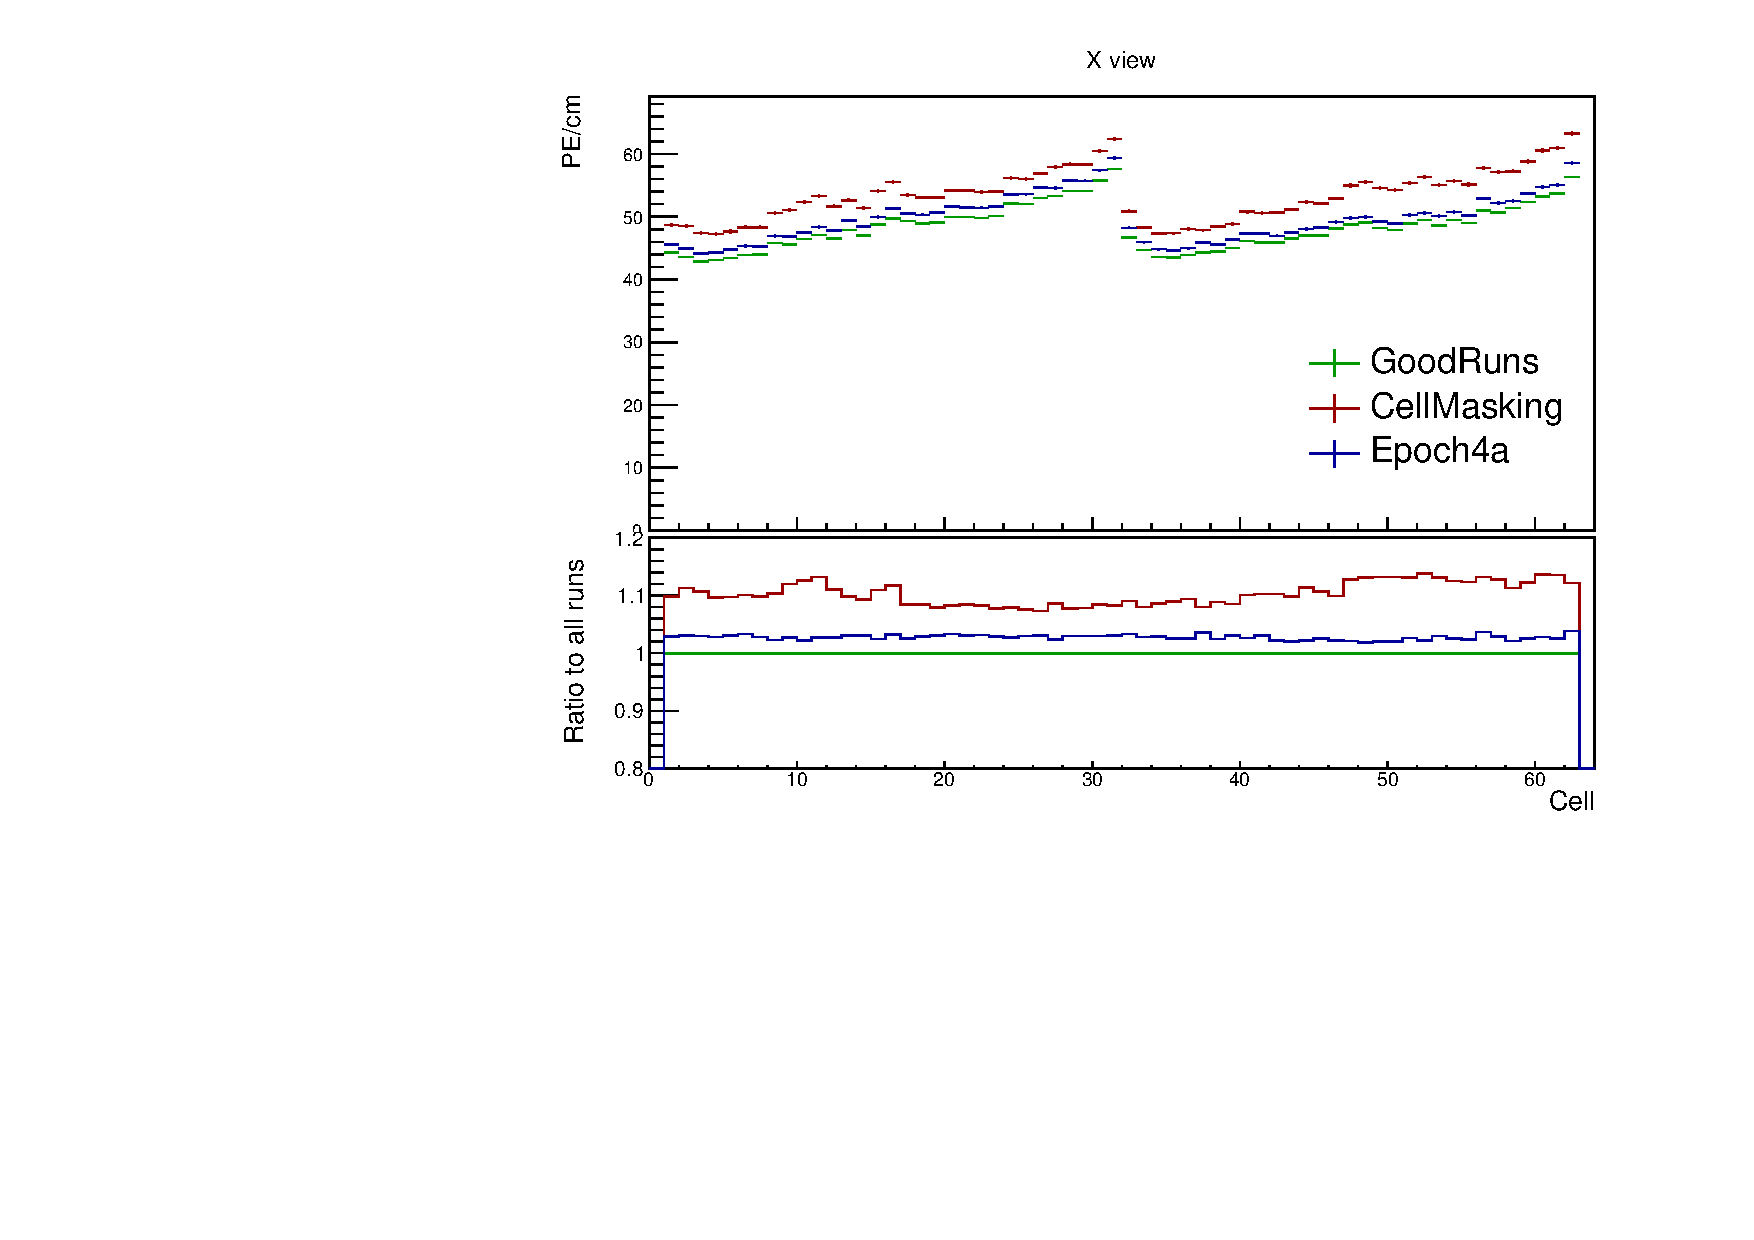
\includegraphics[width=\textwidth]{Plots/Attenprofs_P4Data_CellPE_X_Combined.pdf}
\end{subfigure}
\begin{subfigure}[b]{0.495\textwidth}
\centering
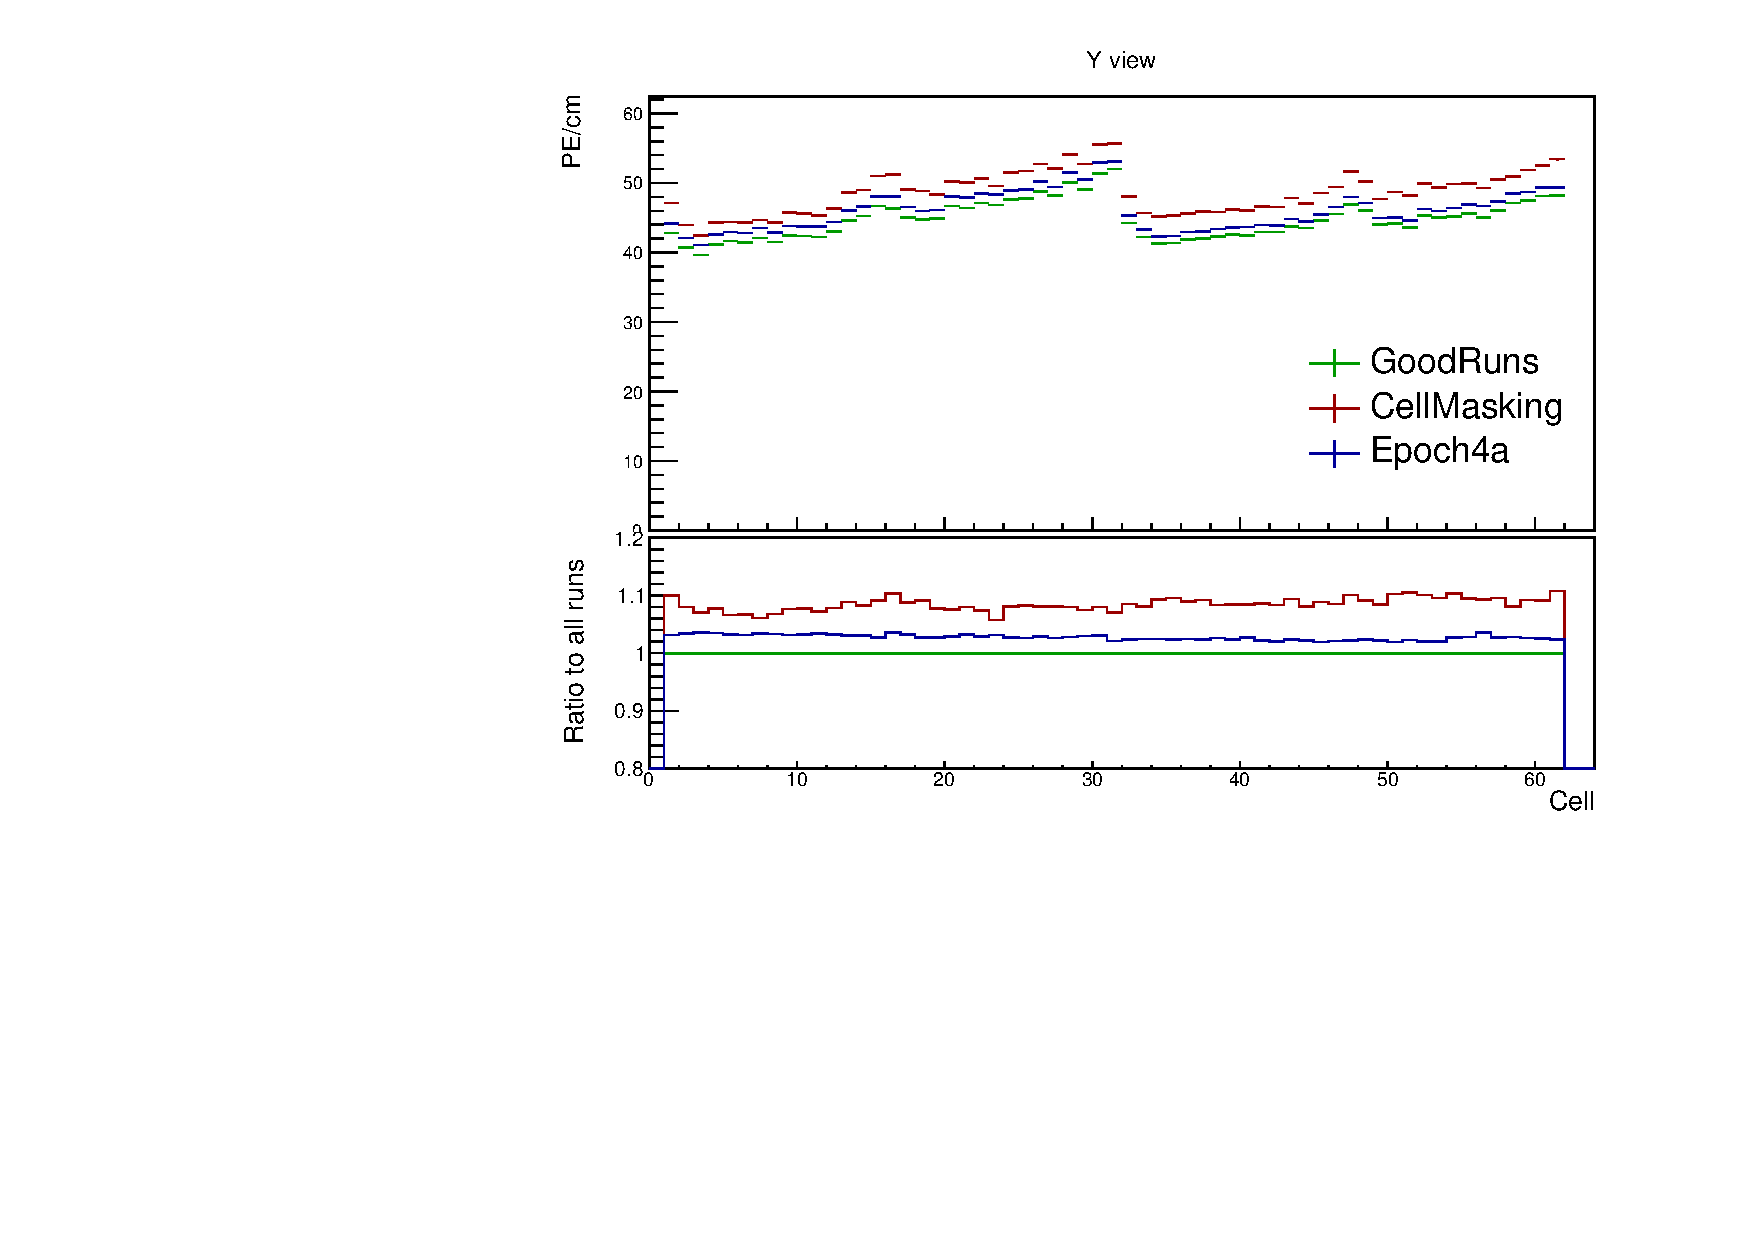
\includegraphics[width=\textwidth]{Plots/Attenprofs_P4Data_CellPE_Y_Combined.pdf}
\end{subfigure}
\caption{Uncorrected average energy response as a function of cells for epochs in period 4.}
\label{figCalibhistCellPE_period4}
\end{figure}

\begin{figure}[!hbtp]
\centering
\begin{subfigure}[b]{0.495\textwidth}
\centering
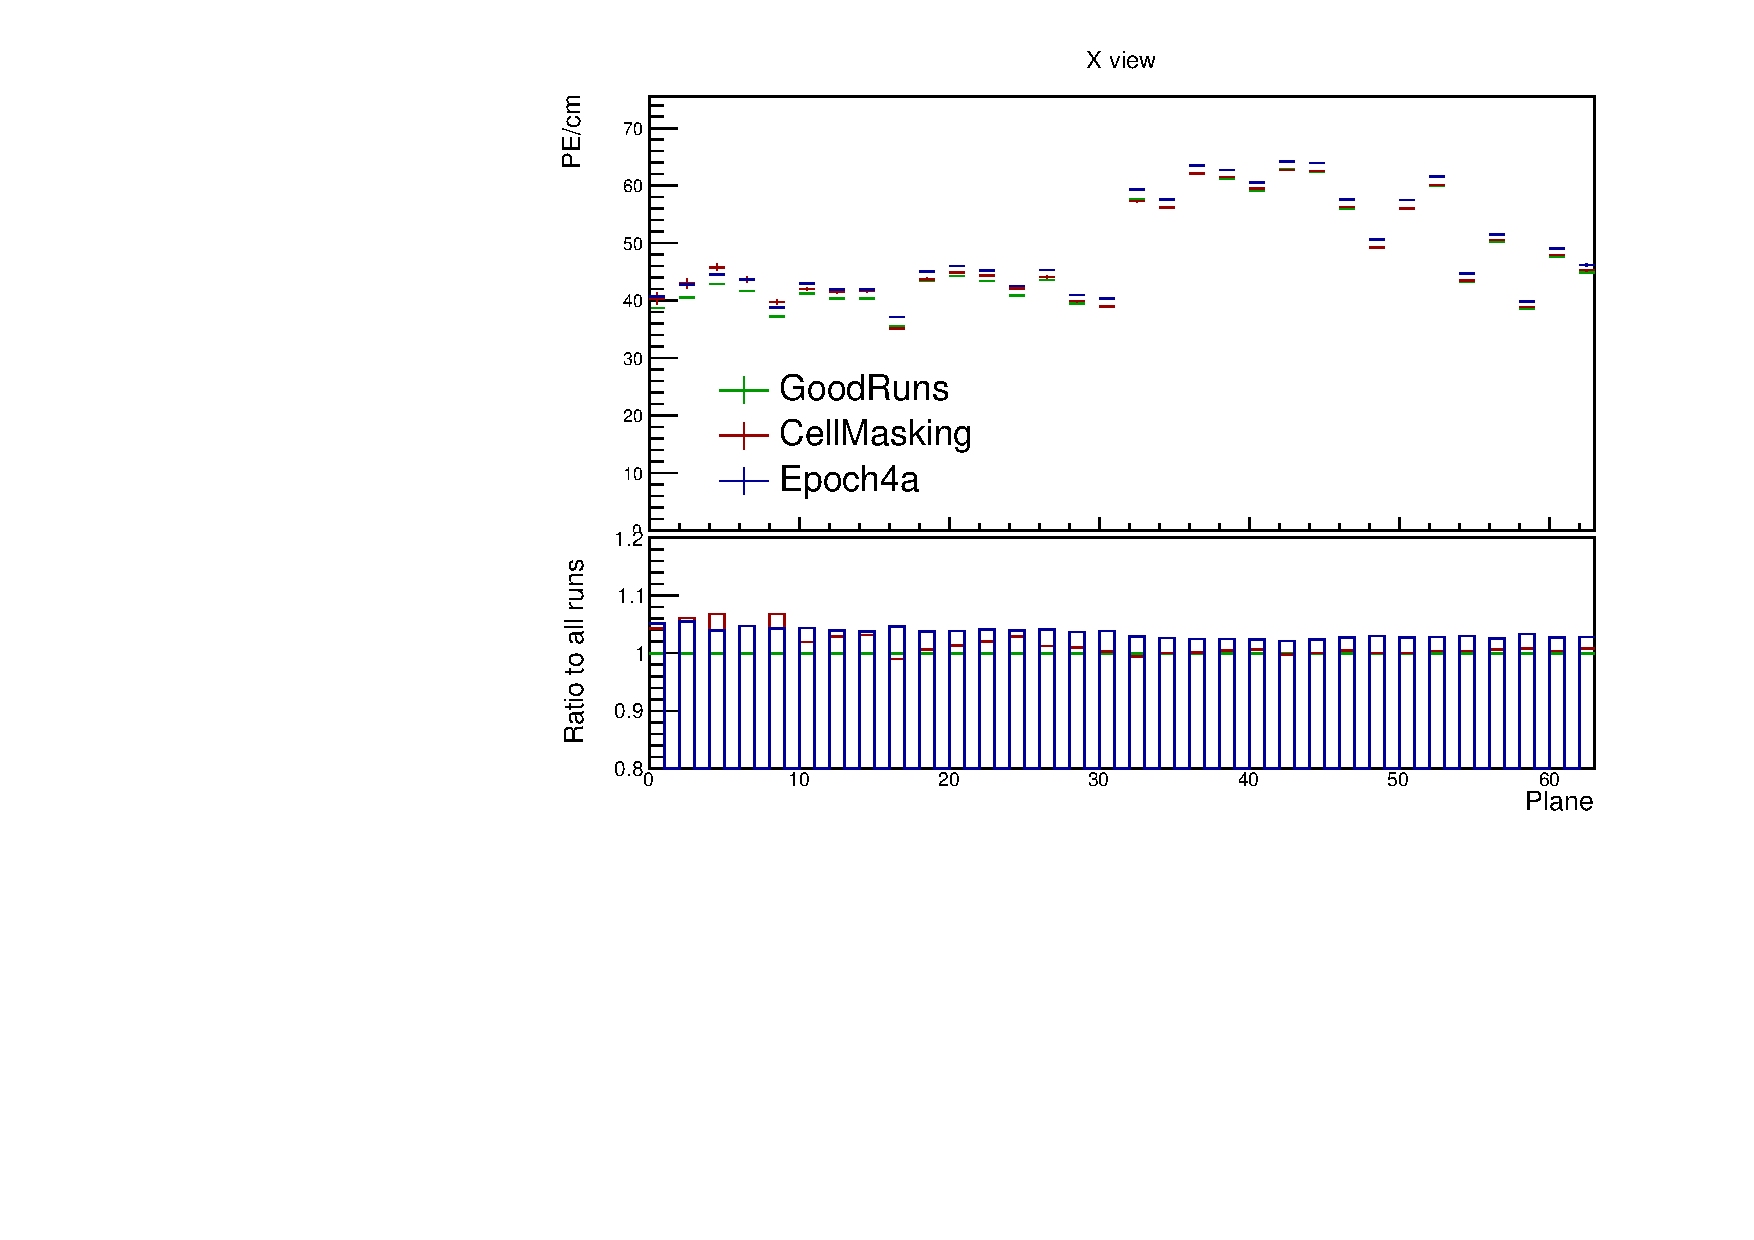
\includegraphics[width=\textwidth]{Plots/Attenprofs_P4Data_PlanePE_X_Combined.pdf}
\end{subfigure}
\begin{subfigure}[b]{0.495\textwidth}
\centering
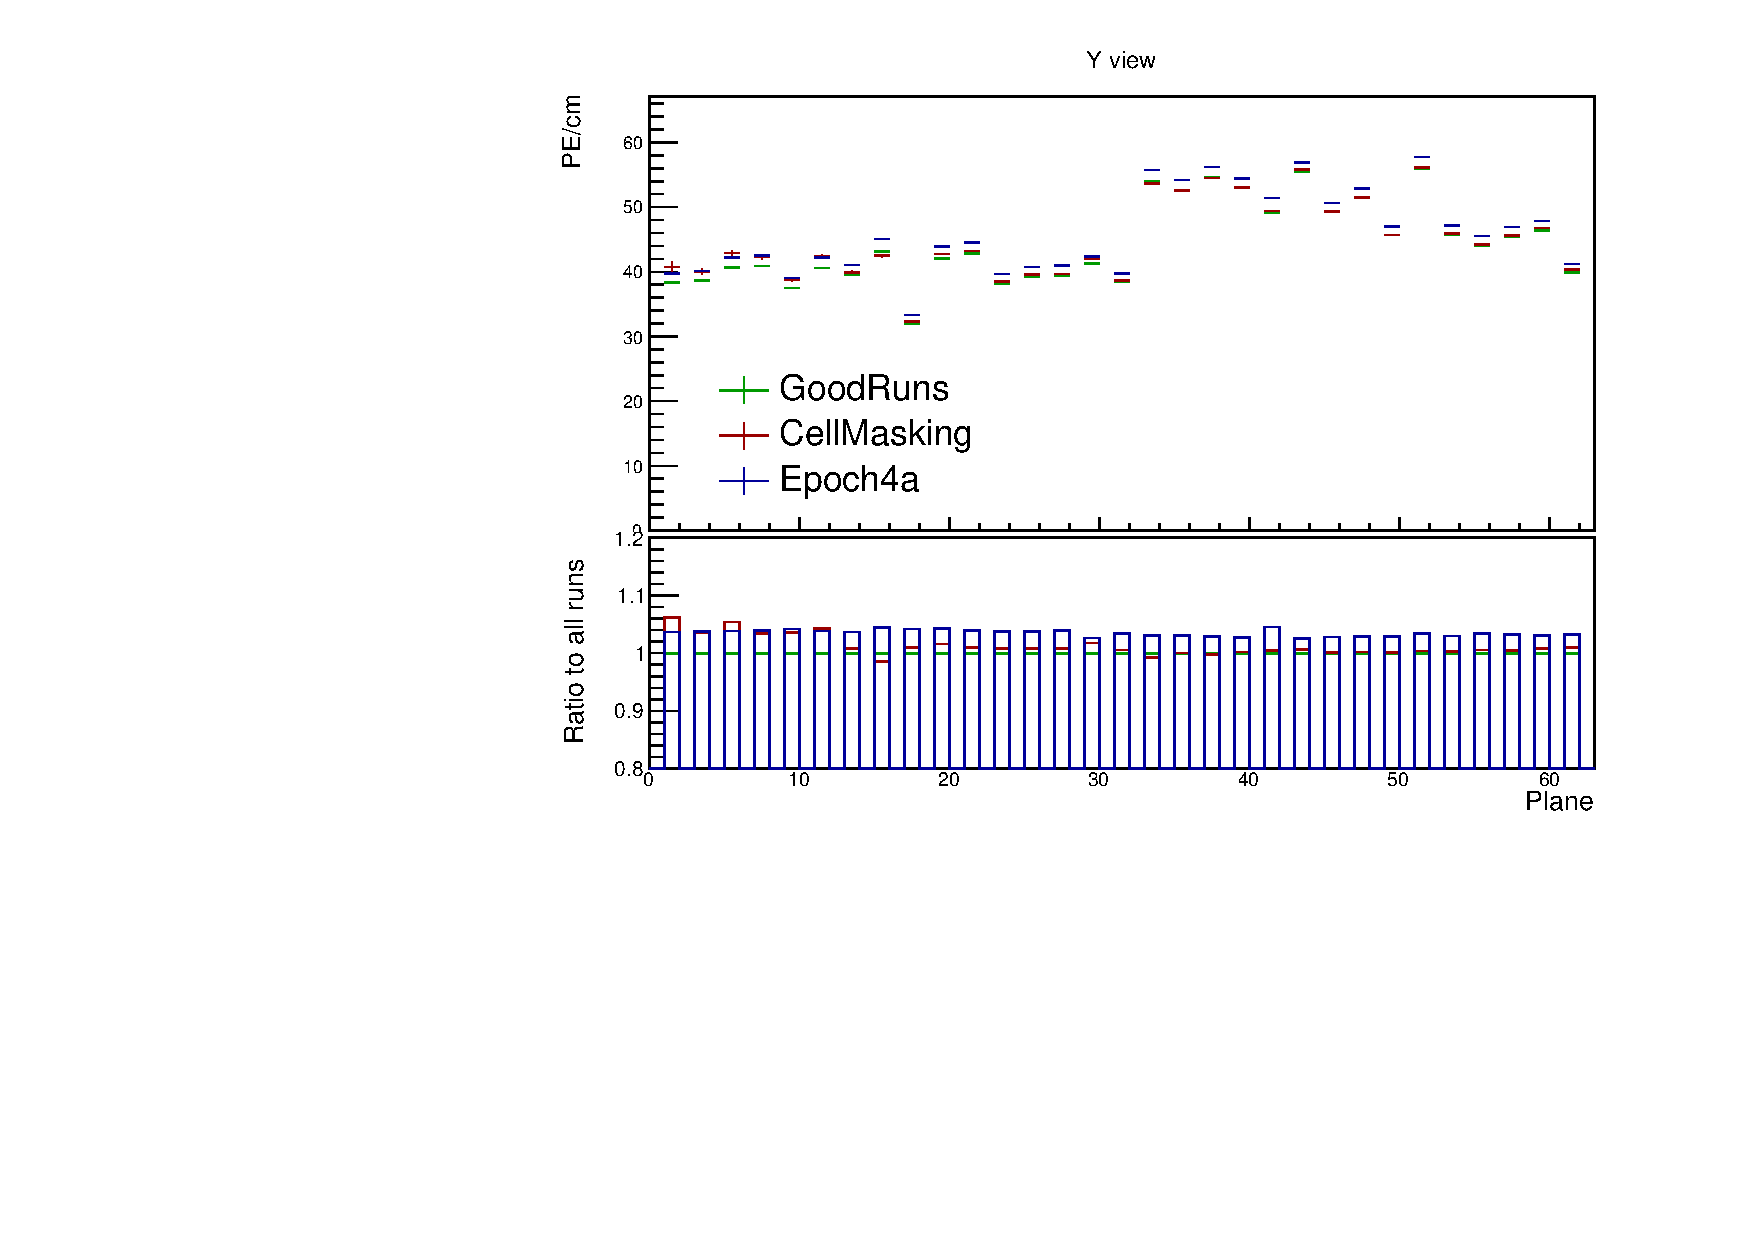
\includegraphics[width=\textwidth]{Plots/Attenprofs_P4Data_PlanePE_Y_Combined.pdf}
\end{subfigure}
\caption{Uncorrected average energy response as a function of planes for epochs in period 4.}
\label{figCalibhistPlanePE_period4}
\end{figure}

\subsubsection{Relative calibration results}

\begin{figure}[!hbtp]
\centering
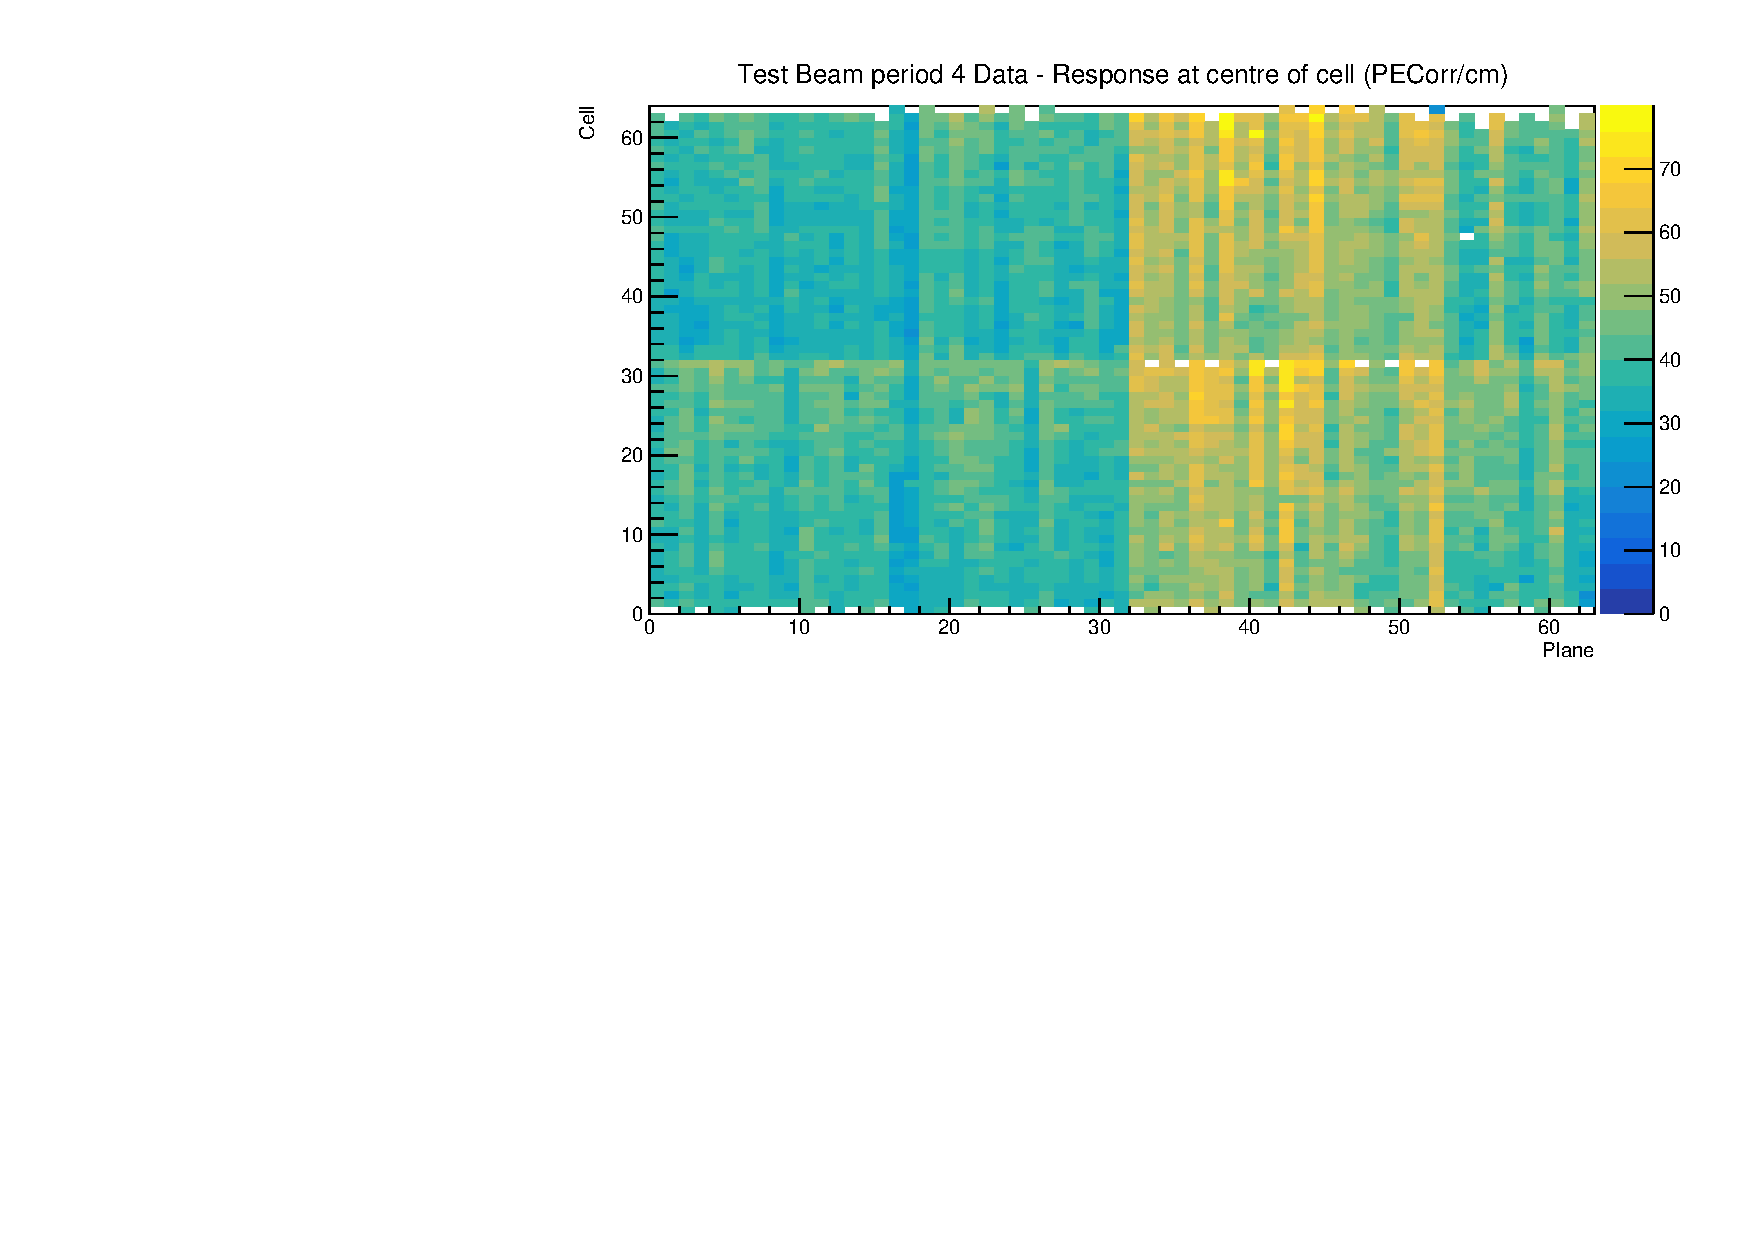
\includegraphics[width=\textwidth]{Plots/CellResponseAtCentre_period4.pdf}
\caption{Overview of the relative calibration results for the Teast Beam detector period 4 data. Each cell is represents the average corrected energy response (in PECorr/cm) in the centre of each cell. The blank cells are uncalibrated.}
\end{figure}


%%%%%%%%%%%%%%%%%%%%%%%%%%%%%%%%%%%%%%%%%%%%%%%%%%%%%%%%%%%%%%%%%%%%%%%%%%%%%%%
%%%%%%%%%%%%%%%%%%%%%%%%%%%%%%%%%%%%%%%%%%%%%%%%%%%%%%%%%%%%%%%%%%%%%%%%%%%%%%%
%%%
%%%                        Absolute calibration results
%%%
%%%%%%%%%%%%%%%%%%%%%%%%%%%%%%%%%%%%%%%%%%%%%%%%%%%%%%%%%%%%%%%%%%%%%%%%%%%%%%%
\subsection{Absolute calibration results}

Standard absolute calibration cuts: track window, flat-response W, positive pe, pecorr, and pathlenght reco\begin{center}
\begin{table}[h!]
\begin{tabular}{ |c|c|c|c|c|c|c|c|c|}

\hline
Sample & NHits$ x$ & MEU$ x$ & NHits$ y$ & MEU$ y$ & MEU & MEU Err & TrueE/dx & tE/dx Err\\ \hline
epoch 3abc data & 2.638e+05 & 38.49 & 1.621e+06 & 39.4 & 38.94 & 0.006758 & 1.772 & 0.000238\\ \hline
epoch 3de data & 1.049e+05 & 38.63 & 6.725e+05 & 39.42 & 39.02 & 0.01048 & 1.772 & 0.000238\\ \hline
period 2 data & 2.322e+05 & 38.7 & 1.413e+06 & 39.4 & 39.05 & 0.007252 & 1.772 & 0.000238\\ \hline
period 4 data & 5.268e+05 & 38.63 & 3.316e+06 & 39.4 & 39.01 & 0.004703 & 1.772 & 0.000238\\ \hline
simulation & 2.829e+05 & 40.17 & 1.842e+06 & 39.93 & 40.05 & 0.006418 & 1.772 & 0.000238\\ \hline
\end{tabular}
\label{tab:calib_summary_table}
\end{table}
\end{center}

\begin{figure}[h!]
  \begin{subfigure}{\textwidth}
  \centering
    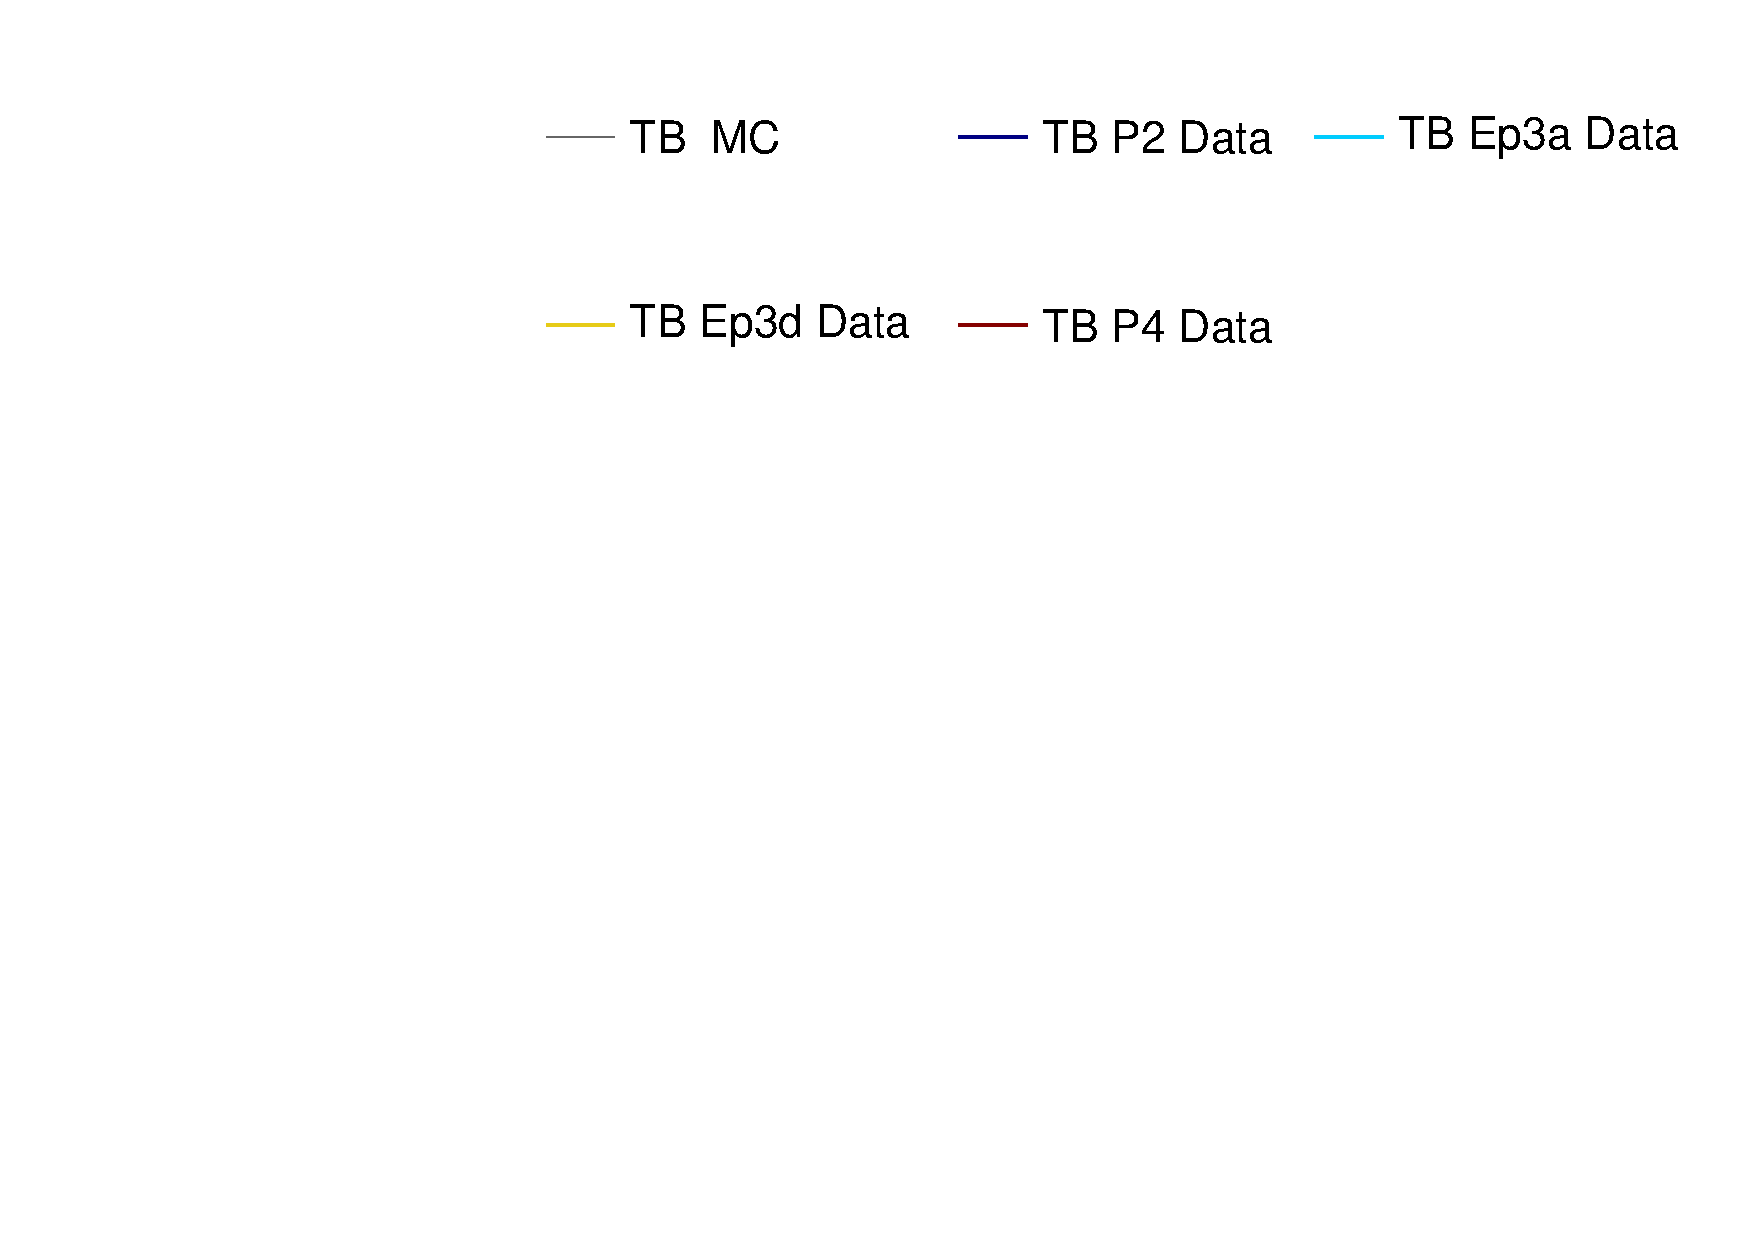
\includegraphics[height=0.2\linewidth]{essentialsec_tb/legend.pdf}
  \end{subfigure}
  \vspace*{2mm}
  
  \begin{subfigure}{0.5\textwidth}
    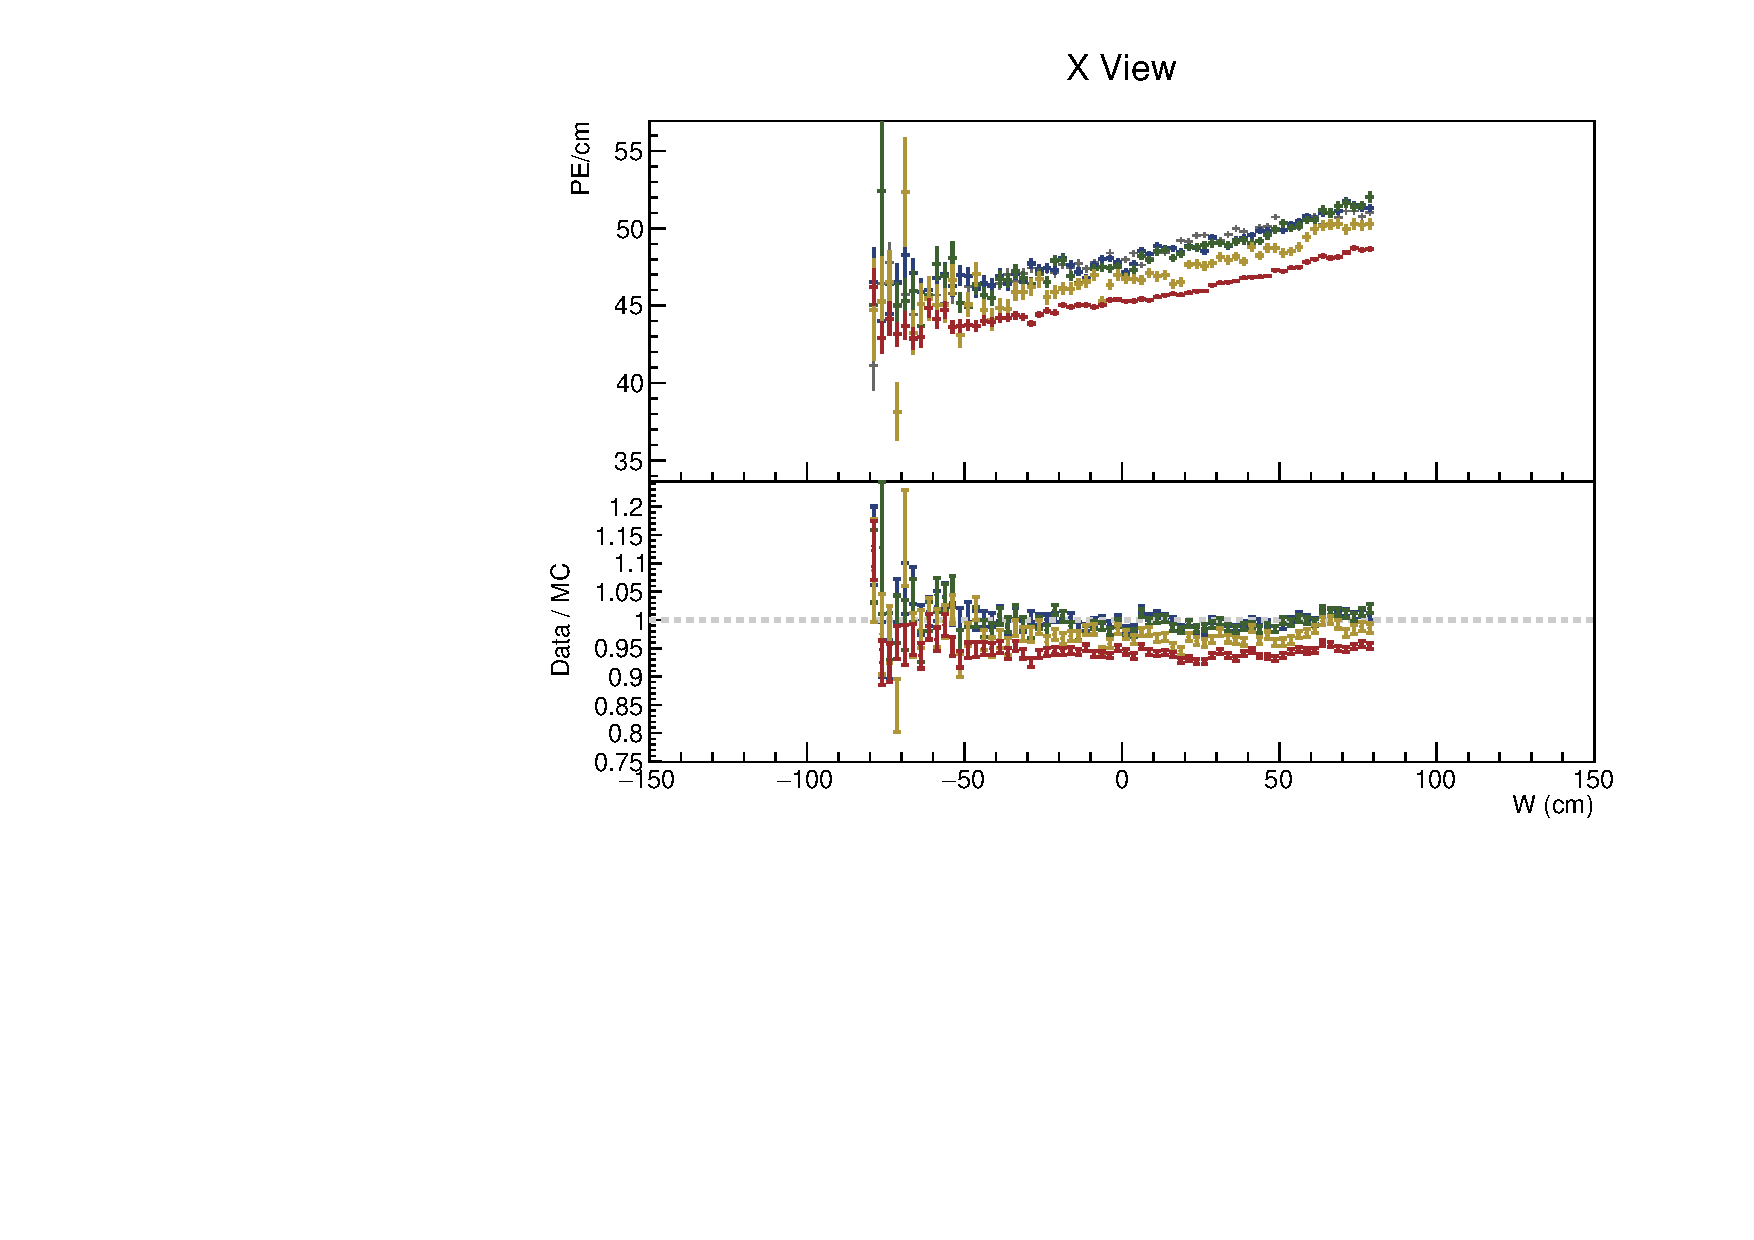
\includegraphics[width=\linewidth]{essentialsec_tb/pecm_w_x.pdf}
  \end{subfigure}
  \begin{subfigure}{0.5\textwidth}
    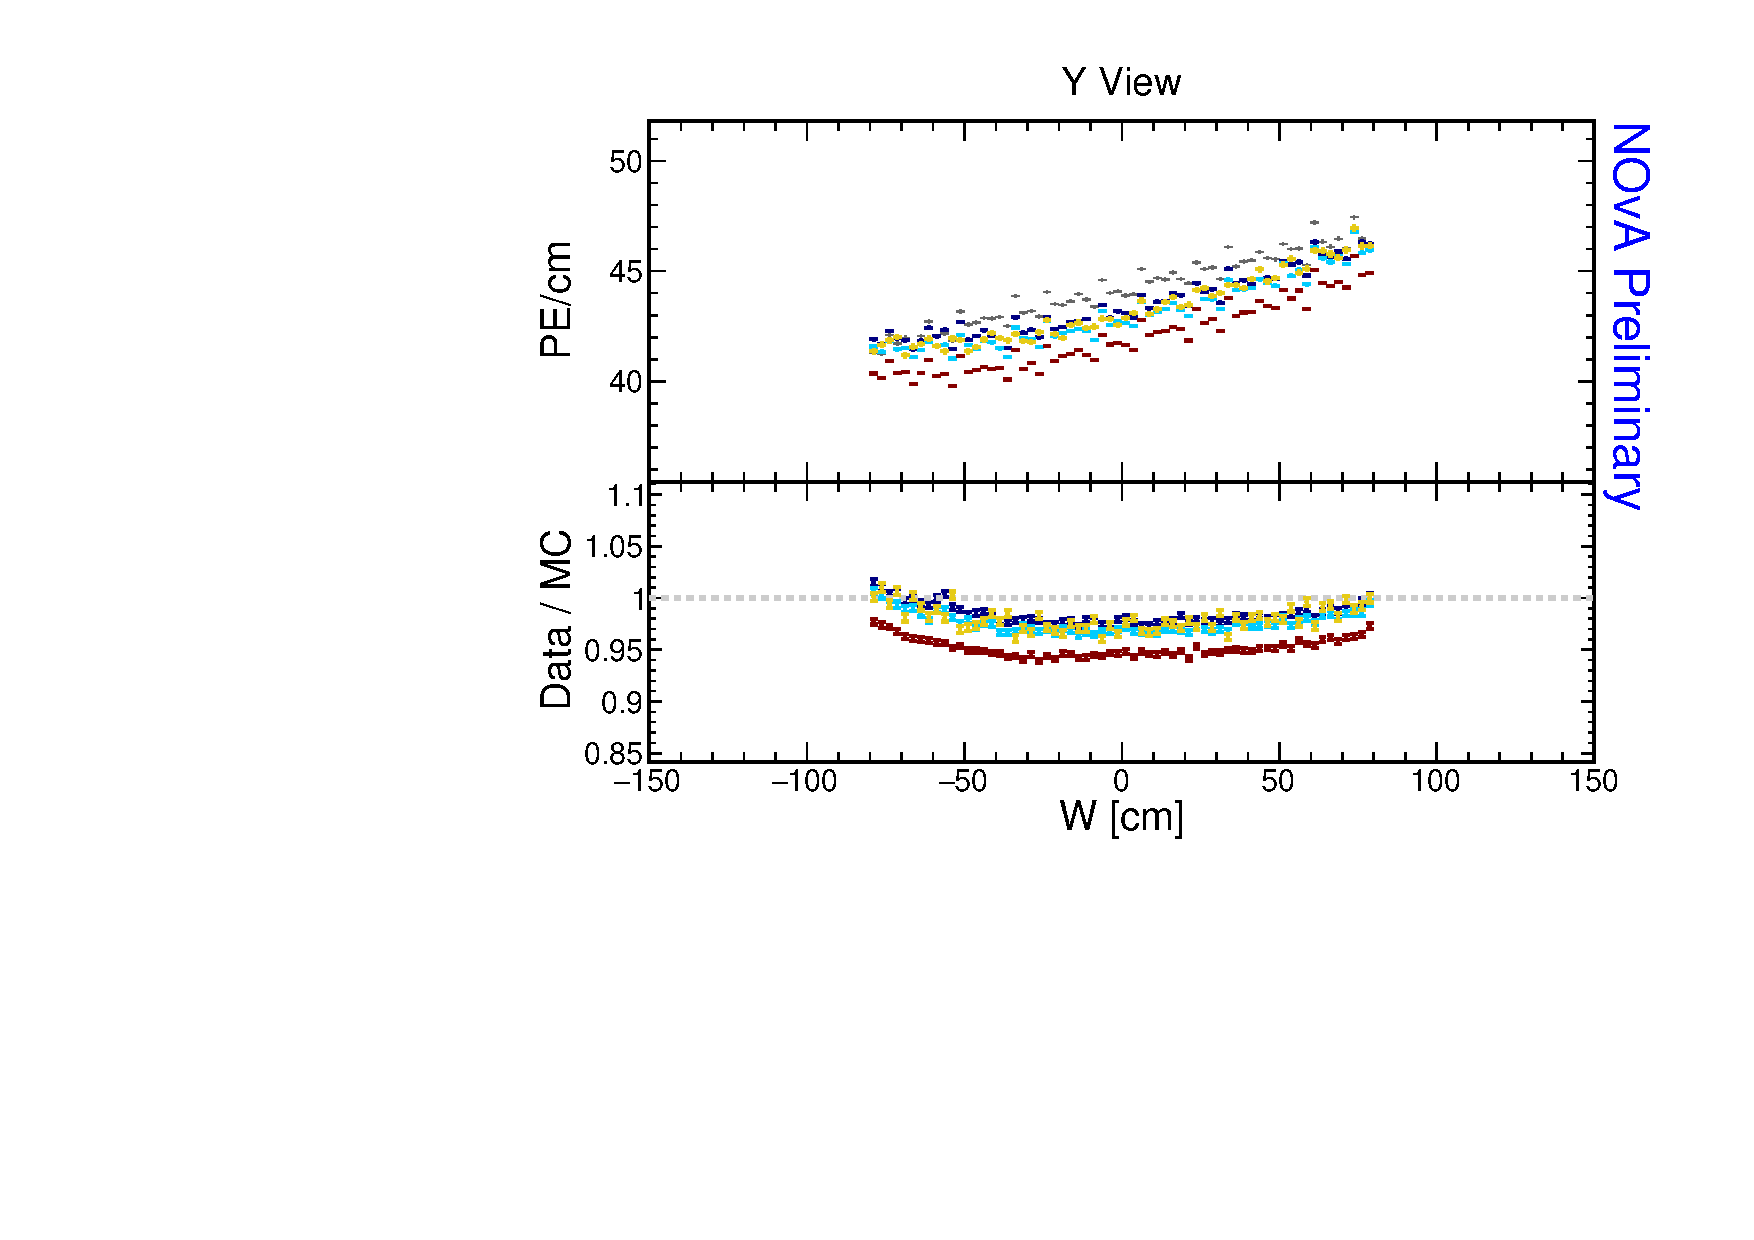
\includegraphics[width=\linewidth]{essentialsec_tb/pecm_w_y.pdf}
  \end{subfigure}
  \begin{subfigure}{0.5\textwidth}
    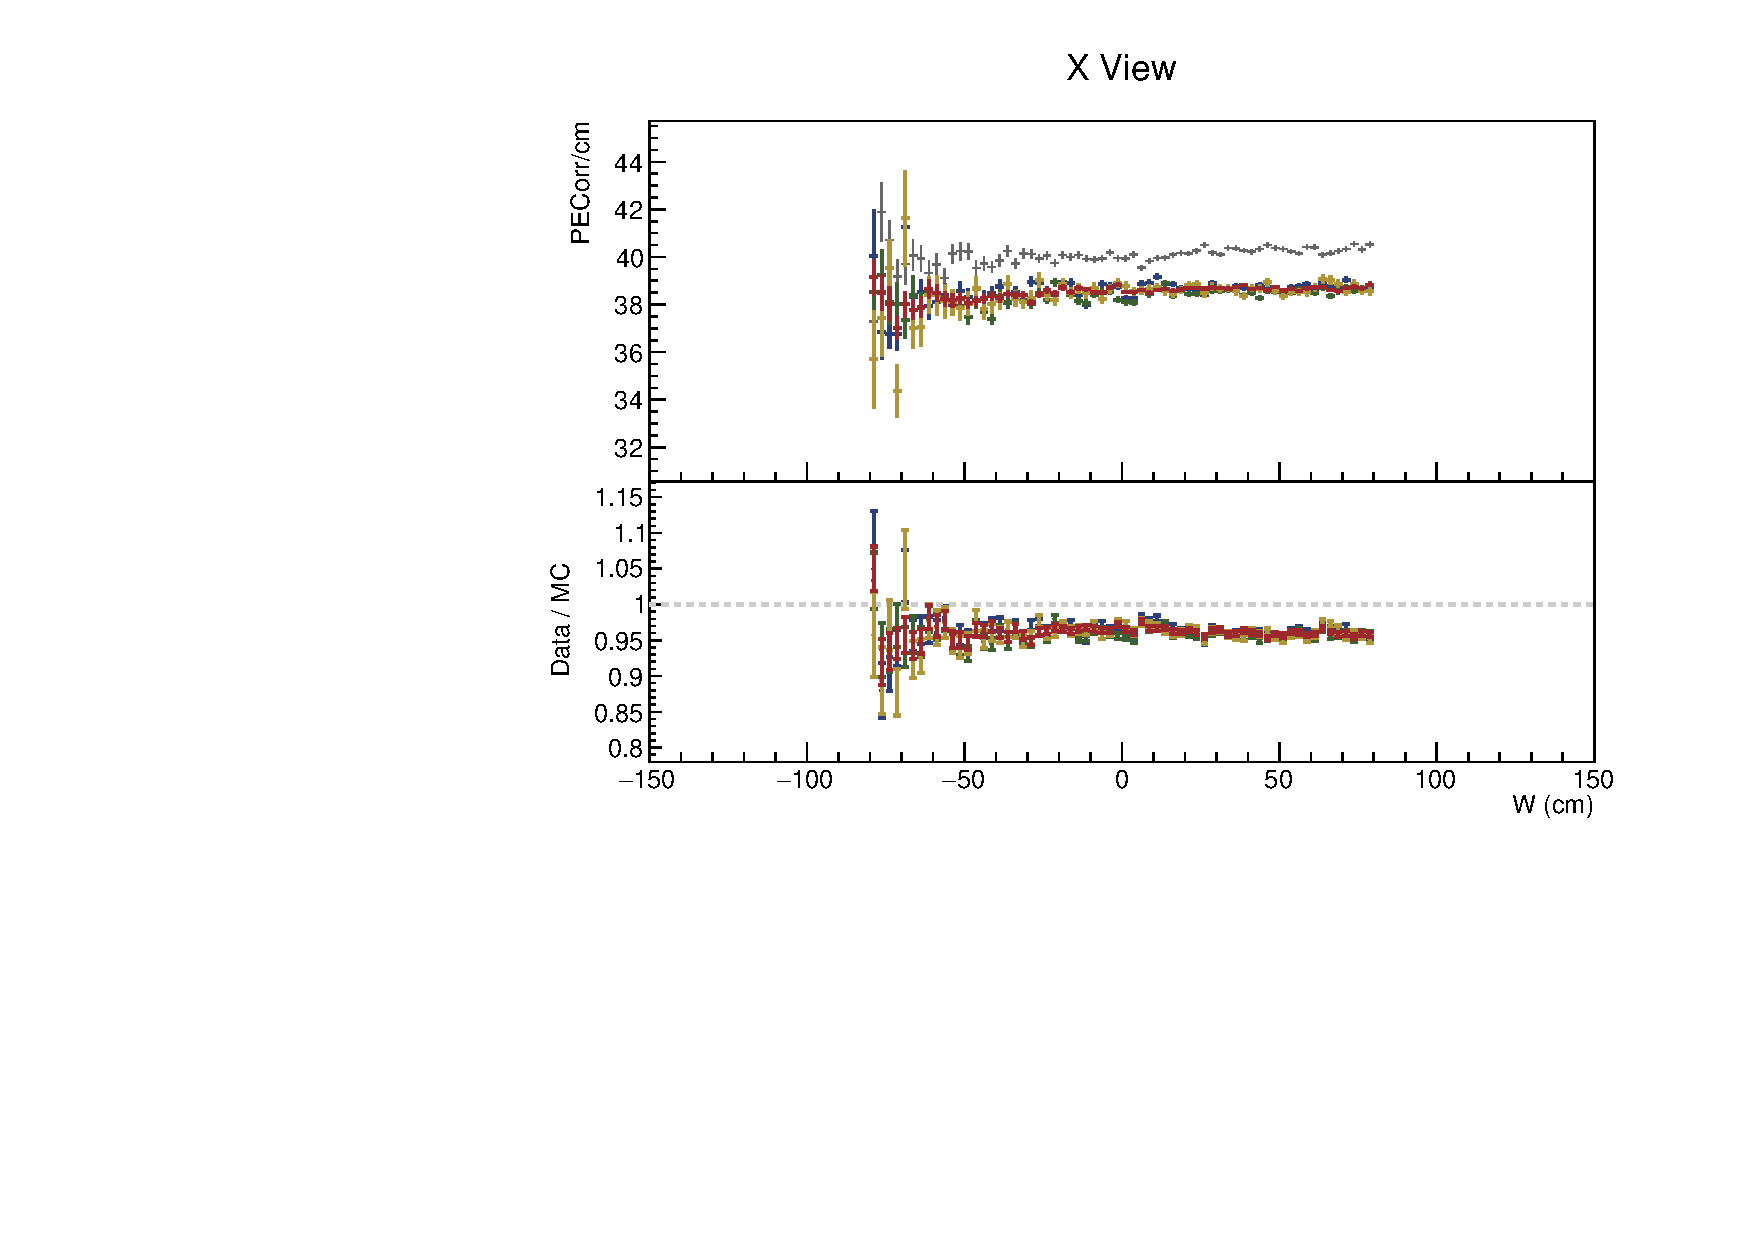
\includegraphics[width=\linewidth]{essentialsec_tb/pecorrcm_w_x.pdf}
  \end{subfigure}
  \begin{subfigure}{0.5\textwidth}
    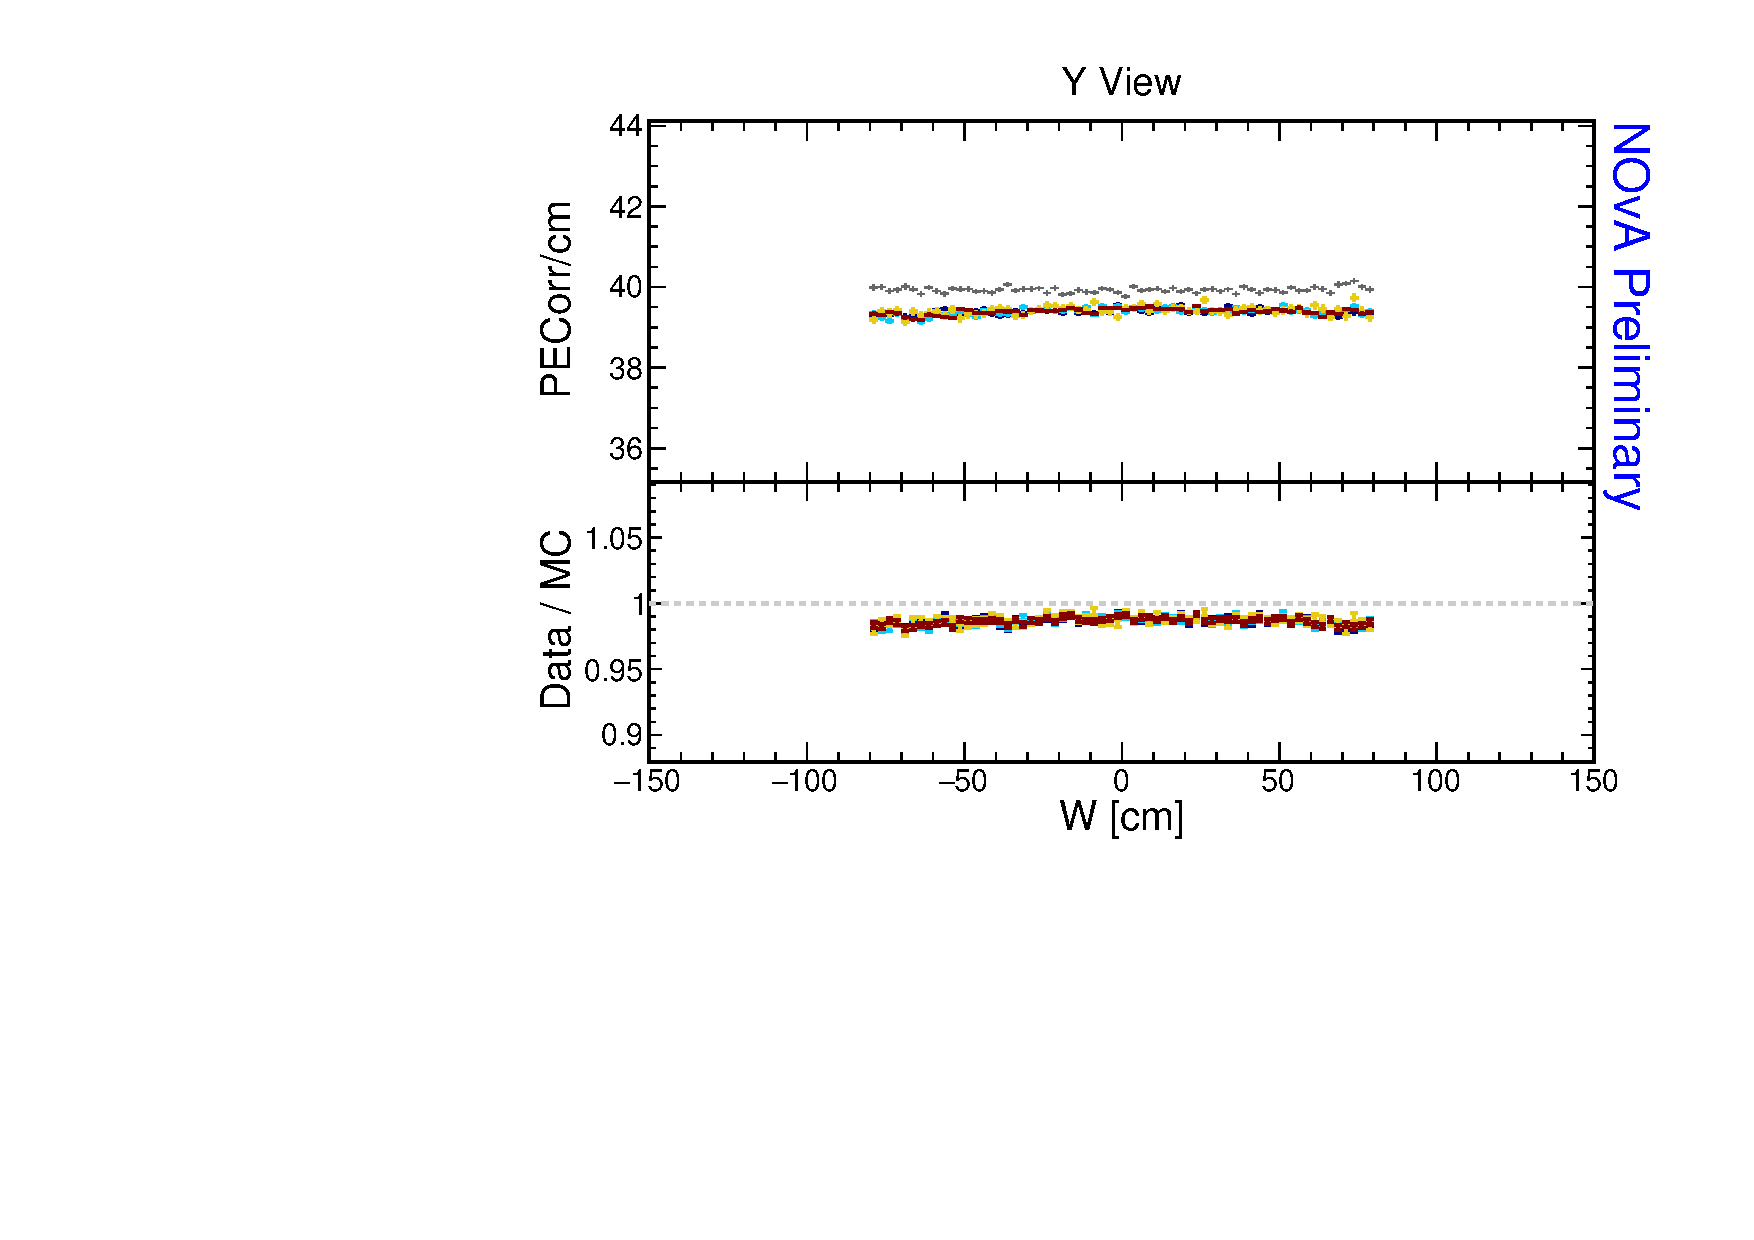
\includegraphics[width=\linewidth]{essentialsec_tb/pecorrcm_w_y.pdf}
  \end{subfigure}
  \caption{...}
  \label{figAbsCalibW1}
\end{figure}

\begin{figure}[h!]
  \begin{subfigure}{\textwidth}
  \centering
    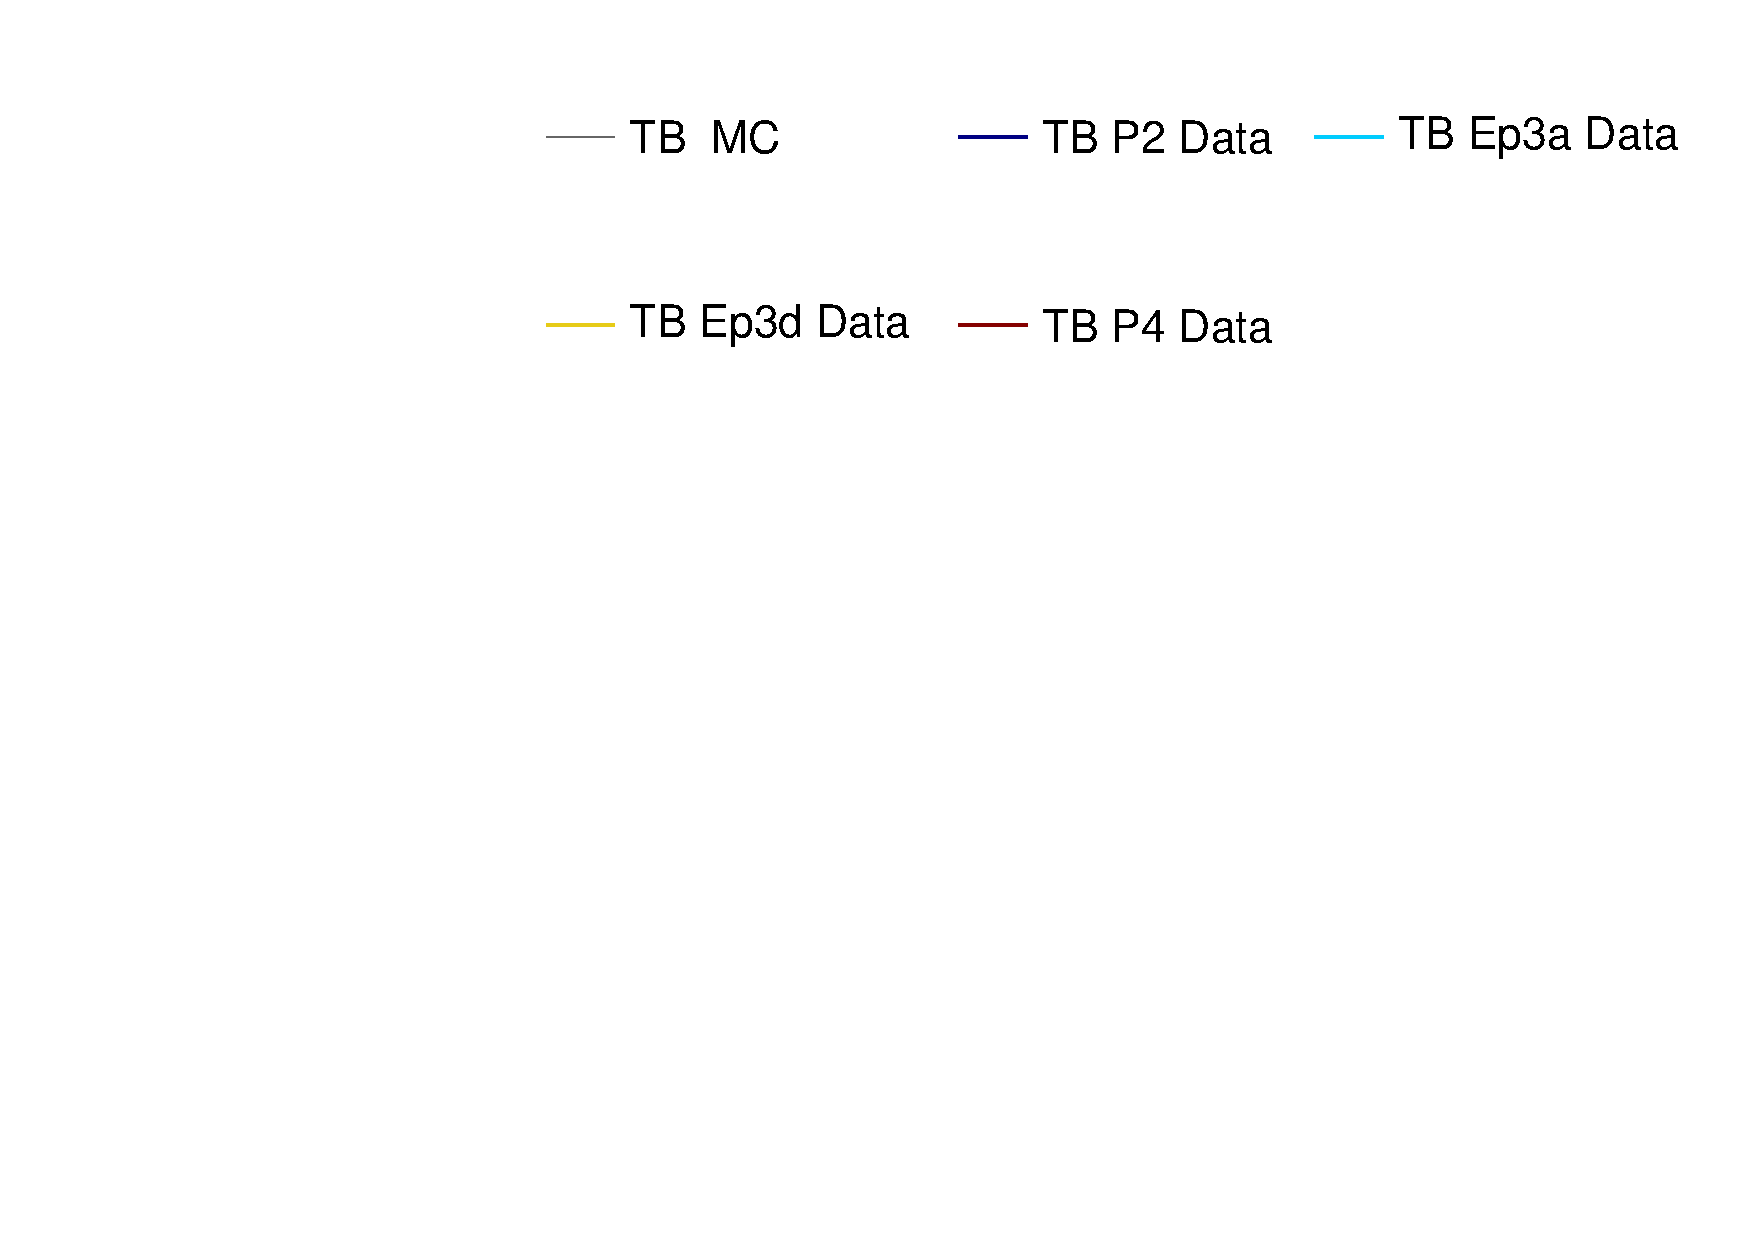
\includegraphics[height=0.2\linewidth]{essentialsec_tb/legend.pdf}
  \end{subfigure}
  \vspace*{2mm}

  \begin{subfigure}{0.5\textwidth}
    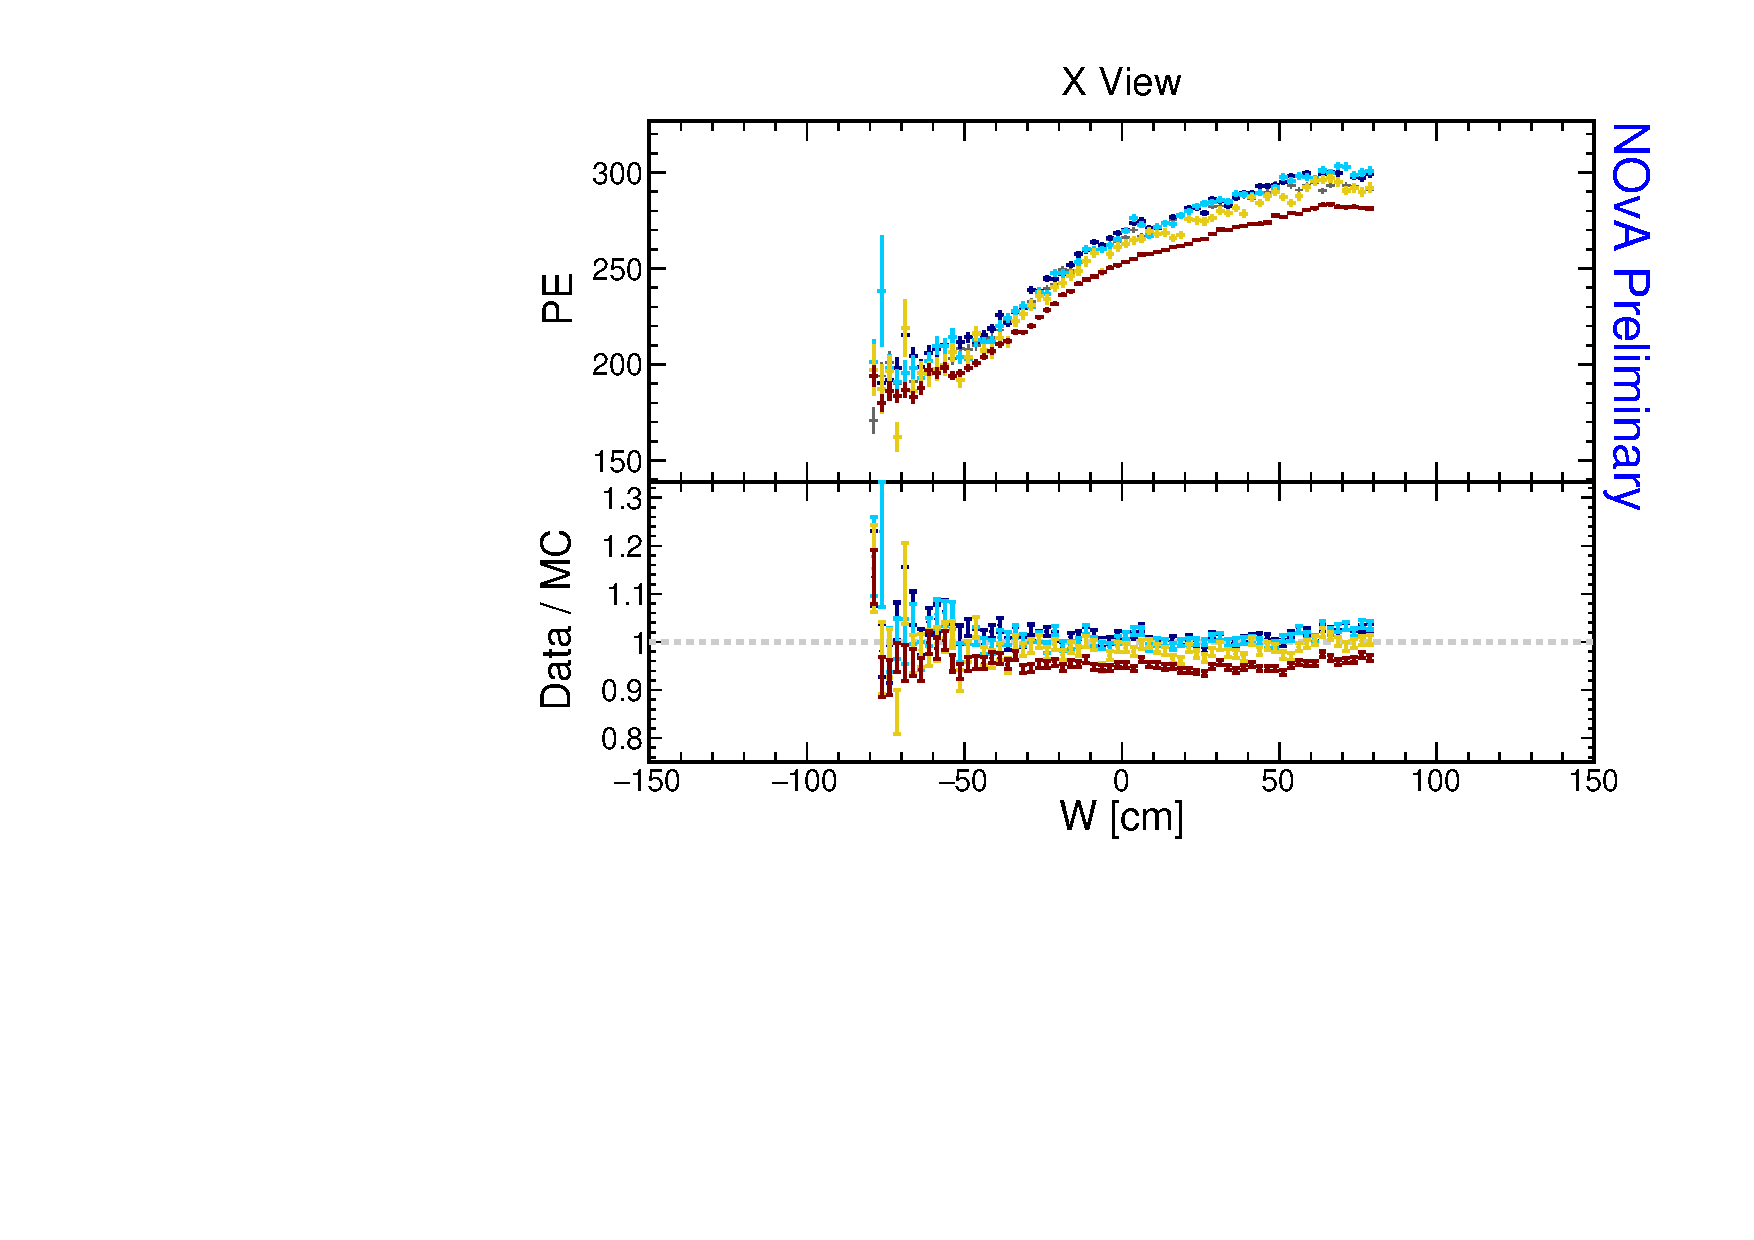
\includegraphics[width=\linewidth]{essentialsec_tb/pe_w_x.pdf}
  \end{subfigure}
  \begin{subfigure}{0.5\textwidth}
    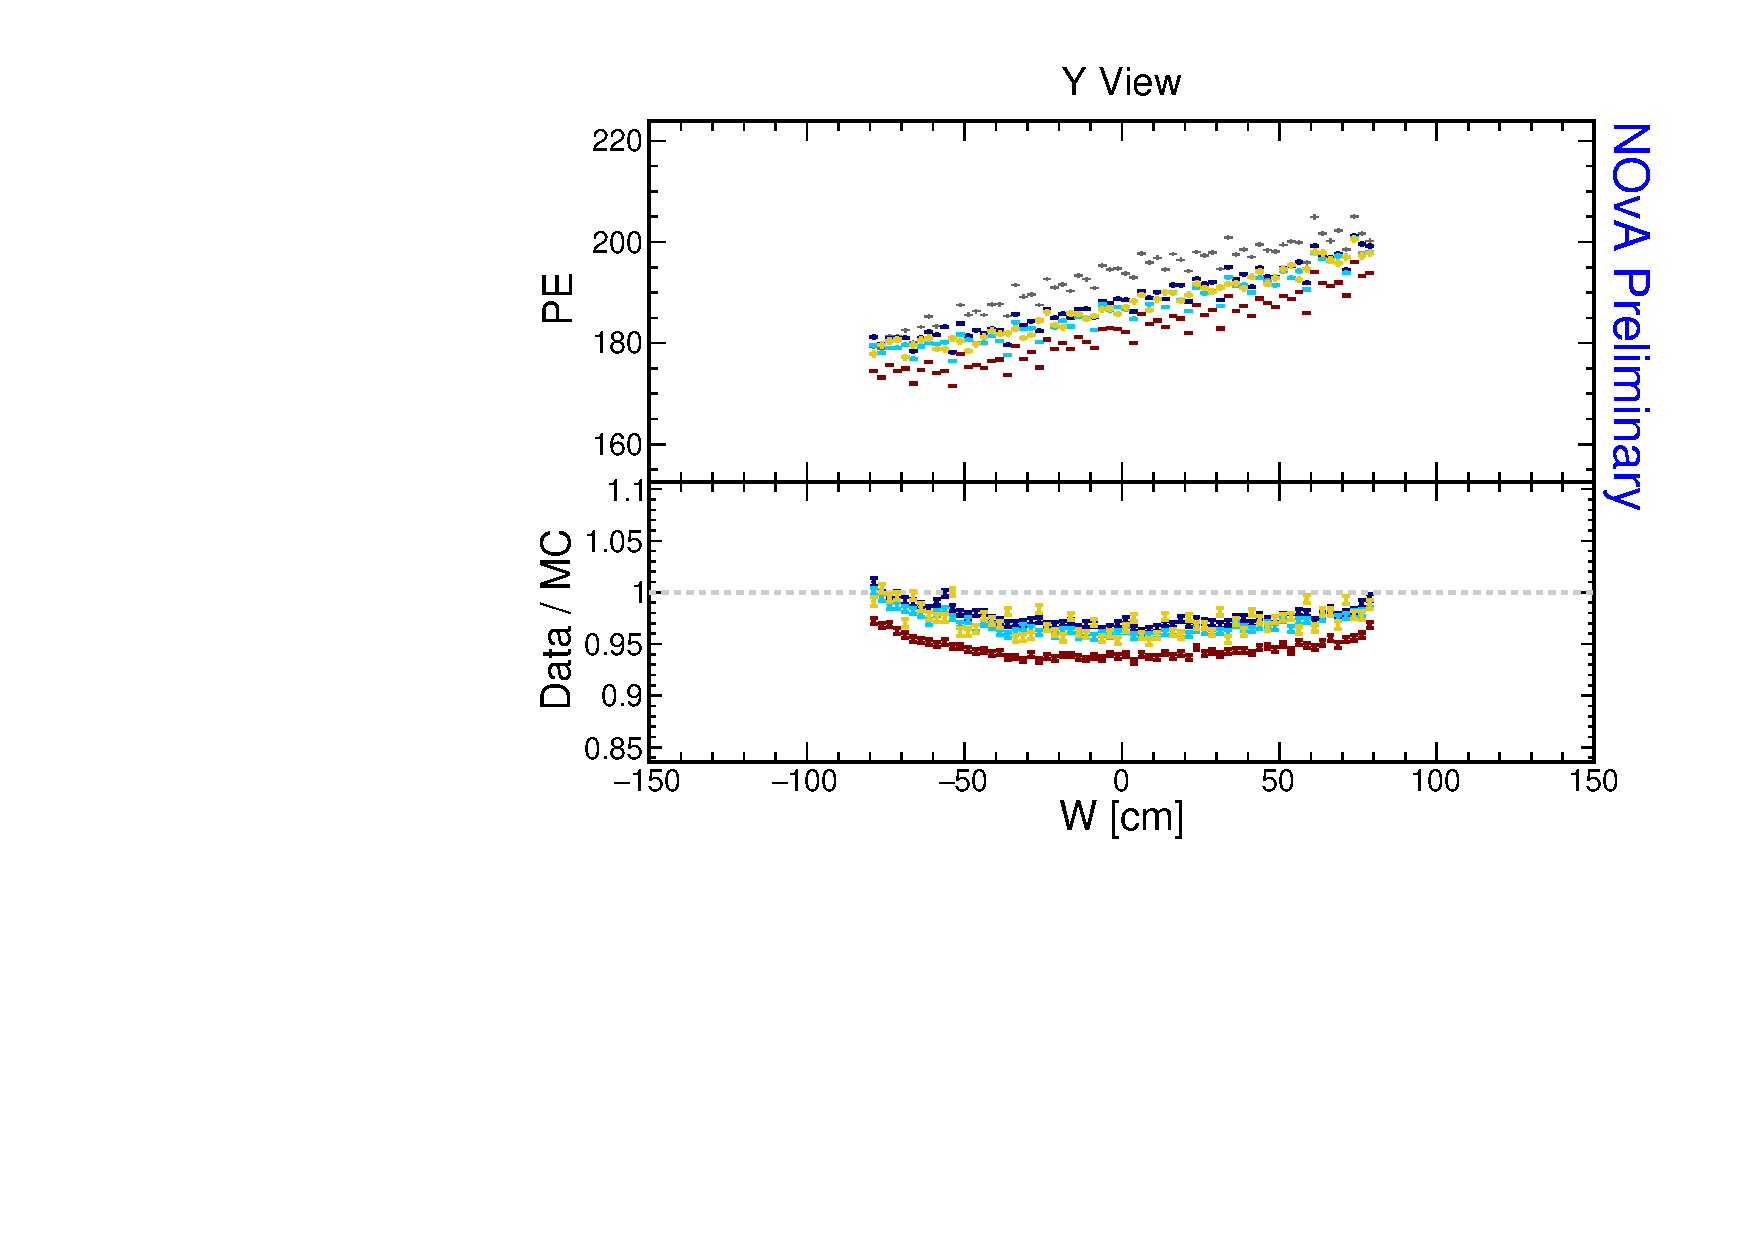
\includegraphics[width=\linewidth]{essentialsec_tb/pe_w_y.pdf}
  \end{subfigure}
  \begin{subfigure}{0.5\textwidth}
    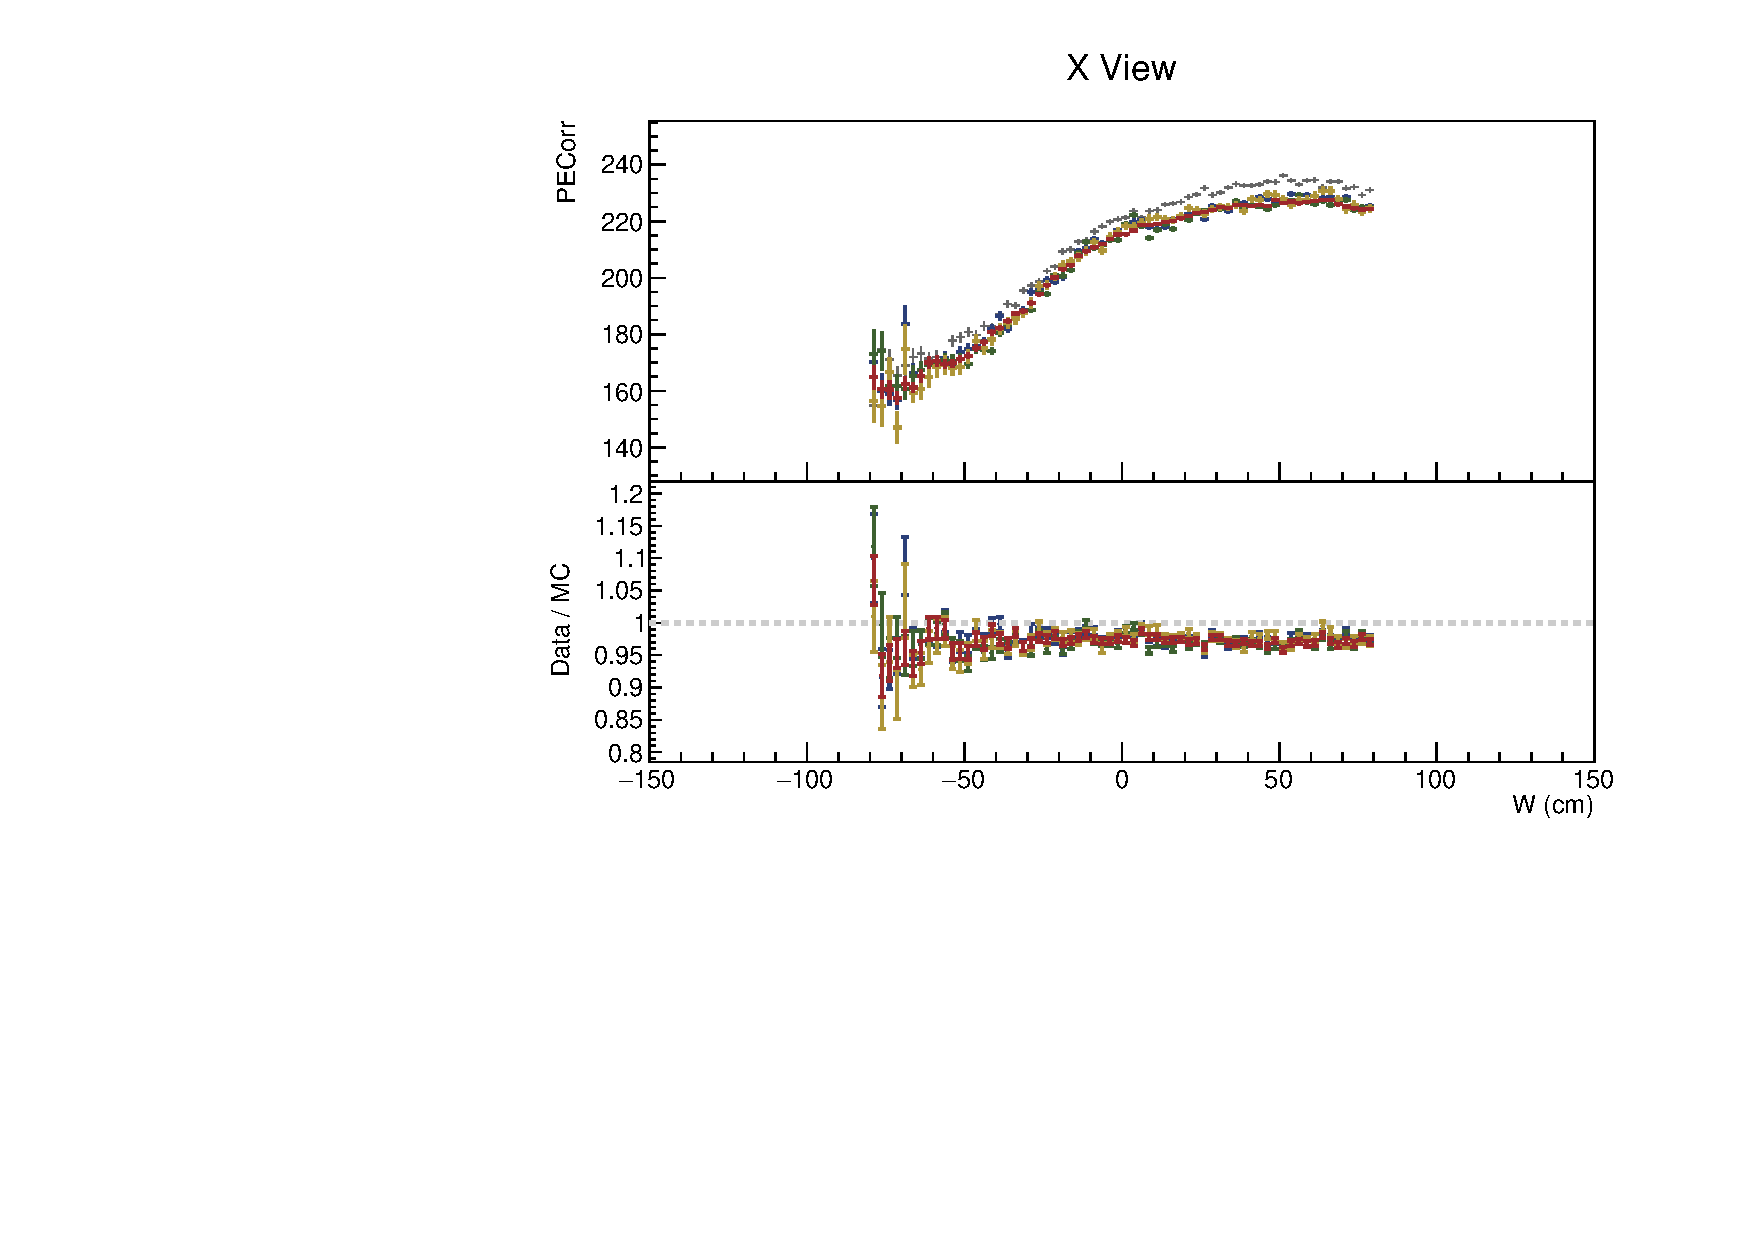
\includegraphics[width=\linewidth]{essentialsec_tb/pecorr_w_x.pdf}
  \end{subfigure}
  \begin{subfigure}{0.5\textwidth}
    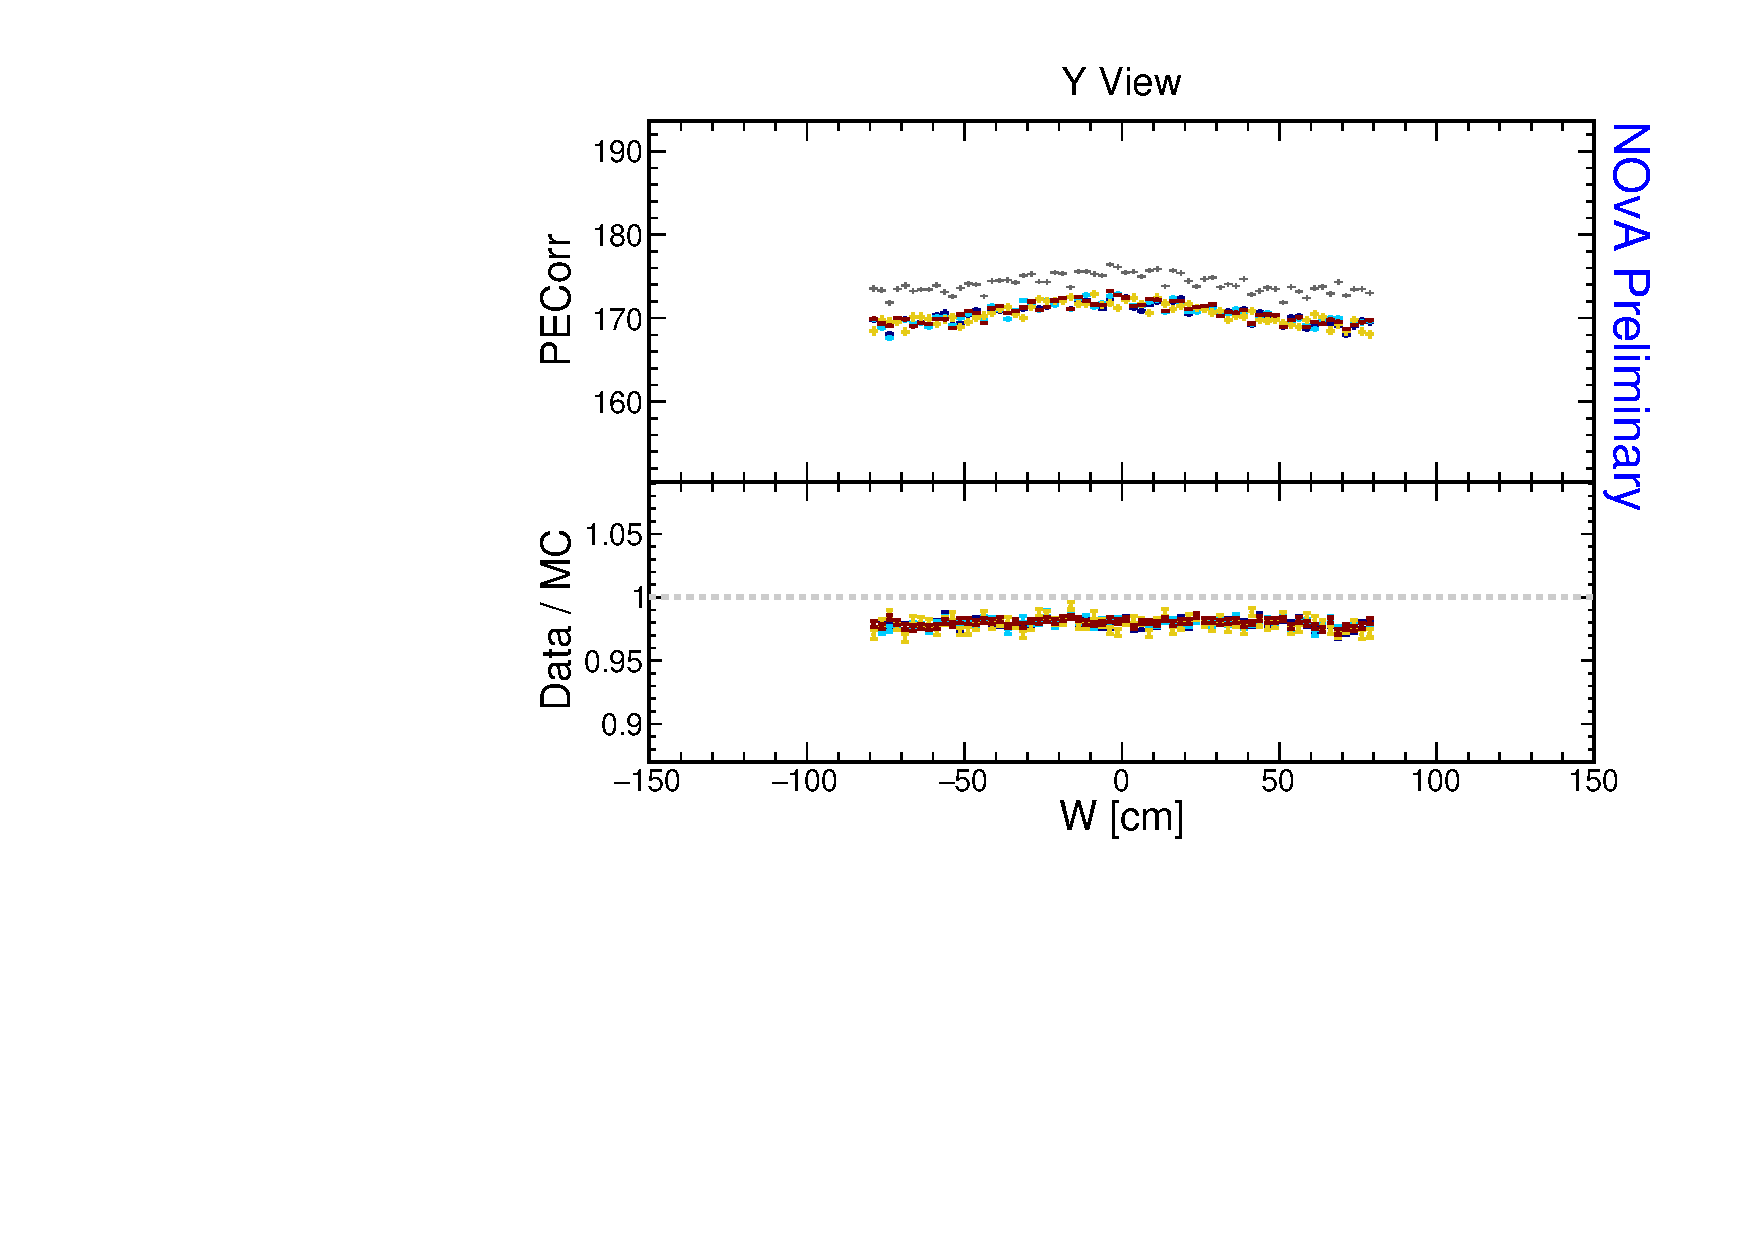
\includegraphics[width=\linewidth]{essentialsec_tb/pecorr_w_y.pdf}
  \end{subfigure}
  \begin{subfigure}{0.5\textwidth}
    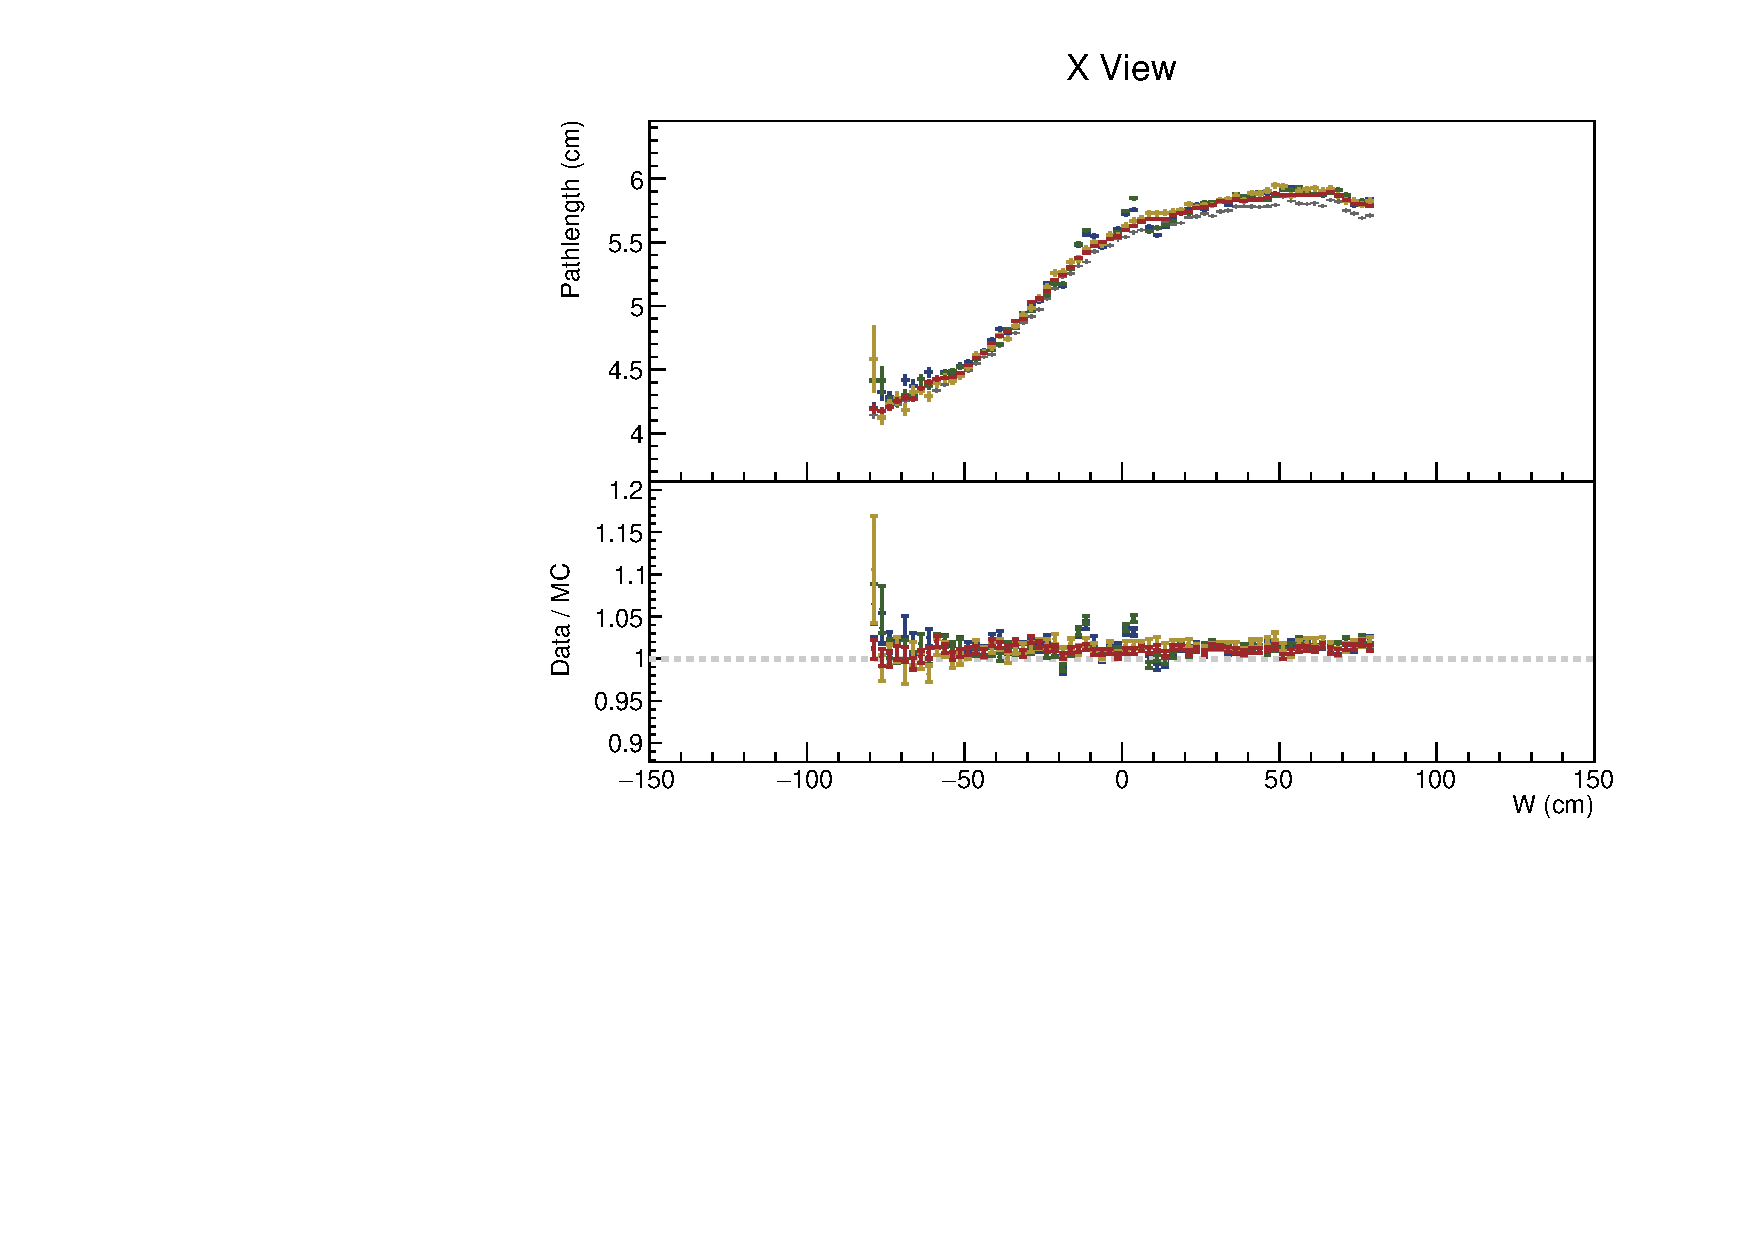
\includegraphics[width=\linewidth]{essentialsec_tb/cm_w_x.pdf}
  \end{subfigure}
  \begin{subfigure}{0.5\textwidth}
    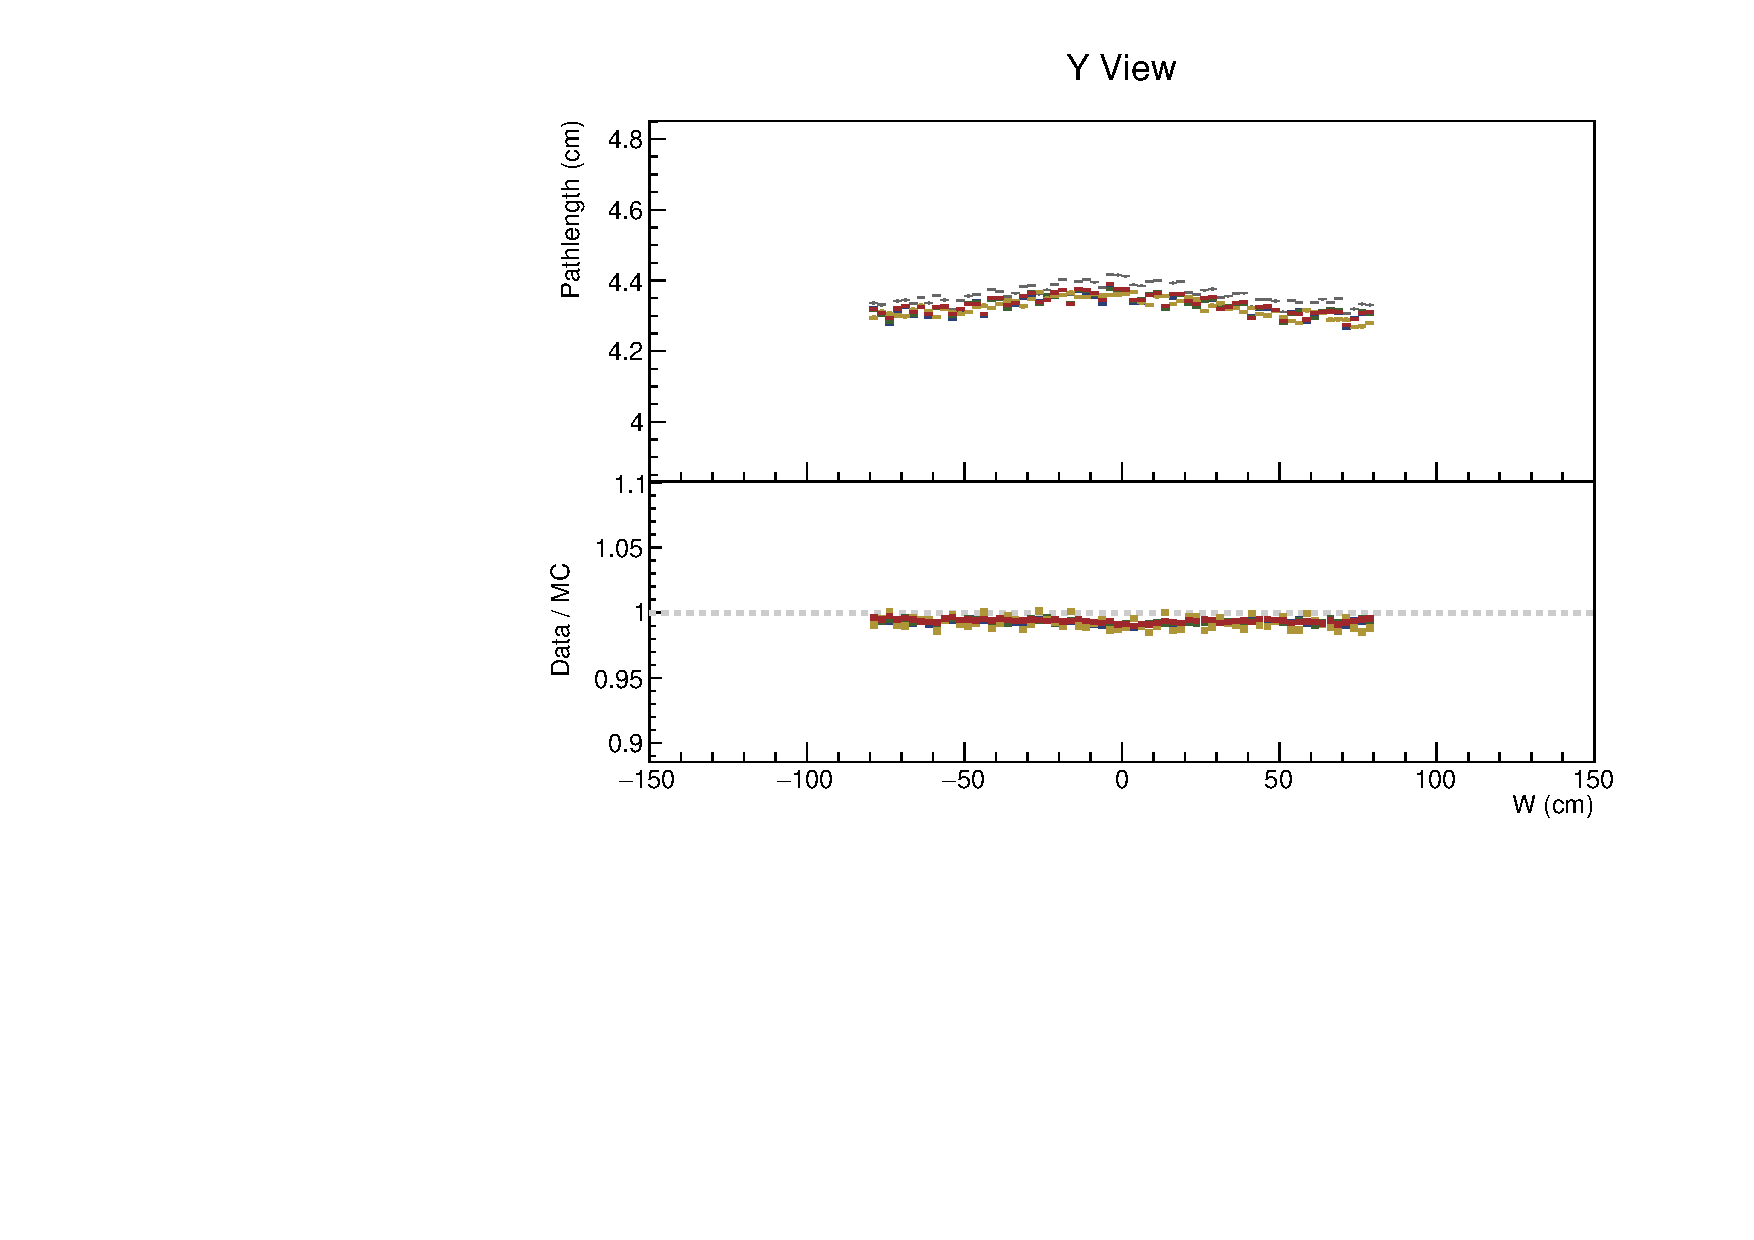
\includegraphics[width=\linewidth]{essentialsec_tb/cm_w_y.pdf}
  \end{subfigure}
  \caption{...}
  \label{figAbsCalibW2}
\end{figure}

\begin{figure}[h!]
  \begin{subfigure}{\textwidth}
  \centering
    \includegraphics[height=0.2\linewidth]{essentialsec_tb/legend.pdf}
  \end{subfigure}
  \vspace*{2mm}

  \begin{subfigure}{0.5\textwidth}
    \includegraphics[width=\linewidth]{essentialsec_tb/pecm_cell_x.pdf}
  \end{subfigure}
  \begin{subfigure}{0.5\textwidth}
    \includegraphics[width=\linewidth]{essentialsec_tb/pecm_cell_y.pdf}
  \end{subfigure}
  \begin{subfigure}{0.5\textwidth}
    \includegraphics[width=\linewidth]{essentialsec_tb/pecorrcm_cell_x.pdf}
  \end{subfigure}
  \begin{subfigure}{0.5\textwidth}
    \includegraphics[width=\linewidth]{essentialsec_tb/pecorrcm_cell_y.pdf}
  \end{subfigure}
  \caption{...}
  \label{figAbsCalibCell1}
\end{figure}

\begin{figure}[h!]
  \begin{subfigure}{\textwidth}
  \centering
    \includegraphics[height=0.2\linewidth]{essentialsec_tb/legend.pdf}
  \end{subfigure}
  \vspace*{2mm}

  \begin{subfigure}{0.5\textwidth}
    \includegraphics[width=\linewidth]{essentialsec_tb/pe_cell_x.pdf}
  \end{subfigure}
  \begin{subfigure}{0.5\textwidth}
    \includegraphics[width=\linewidth]{essentialsec_tb/pe_cell_y.pdf}
  \end{subfigure}
  \begin{subfigure}{0.5\textwidth}
    \includegraphics[width=\linewidth]{essentialsec_tb/pecorr_cell_x.pdf}
  \end{subfigure}
  \begin{subfigure}{0.5\textwidth}
    \includegraphics[width=\linewidth]{essentialsec_tb/pecorr_cell_y.pdf}
  \end{subfigure}
  \begin{subfigure}{0.5\textwidth}
    \includegraphics[width=\linewidth]{essentialsec_tb/cm_cell_x.pdf}
  \end{subfigure}
  \begin{subfigure}{0.5\textwidth}
    \includegraphics[width=\linewidth]{essentialsec_tb/cm_cell_y.pdf}
  \end{subfigure}
  \caption{...}
  \label{figAbsCalibCell2}
\end{figure}

\begin{figure}[h!]
  \begin{subfigure}{\textwidth}
  \centering
    \includegraphics[height=0.2\linewidth]{essentialsec_tb/legend.pdf}
  \end{subfigure}
  \vspace*{2mm}

  \begin{subfigure}{0.5\textwidth}
    \includegraphics[width=\linewidth]{essentialsec_tb/pecm_plane_x.pdf}
  \end{subfigure}
  \begin{subfigure}{0.5\textwidth}
    \includegraphics[width=\linewidth]{essentialsec_tb/pecm_plane_y.pdf}
  \end{subfigure}
  \begin{subfigure}{0.5\textwidth}
    \includegraphics[width=\linewidth]{essentialsec_tb/pecorrcm_plane_x.pdf}
  \end{subfigure}
  \begin{subfigure}{0.5\textwidth}
    \includegraphics[width=\linewidth]{essentialsec_tb/pecorrcm_plane_y.pdf}
  \end{subfigure}
  \caption{...}
  \label{figAbsCalibPlane1}
\end{figure}

\begin{figure}[h!]
  \begin{subfigure}{\textwidth}
  \centering
    \includegraphics[height=0.2\linewidth]{essentialsec_tb/legend.pdf}
  \end{subfigure}
  \vspace*{2mm}

  \begin{subfigure}{0.5\textwidth}
    \includegraphics[width=\linewidth]{essentialsec_tb/pe_plane_x.pdf}
  \end{subfigure}
  \begin{subfigure}{0.5\textwidth}
    \includegraphics[width=\linewidth]{essentialsec_tb/pe_plane_y.pdf}
  \end{subfigure}
  \begin{subfigure}{0.5\textwidth}
    \includegraphics[width=\linewidth]{essentialsec_tb/pecorr_plane_x.pdf}
  \end{subfigure}
  \begin{subfigure}{0.5\textwidth}
    \includegraphics[width=\linewidth]{essentialsec_tb/pecorr_plane_y.pdf}
  \end{subfigure}
  \begin{subfigure}{0.5\textwidth}
    \includegraphics[width=\linewidth]{essentialsec_tb/cm_plane_x.pdf}
  \end{subfigure}
  \begin{subfigure}{0.5\textwidth}
    \includegraphics[width=\linewidth]{essentialsec_tb/cm_plane_y.pdf}
  \end{subfigure}
  \caption{...}
  \label{figAbsCalibPlane2}
\end{figure}

\begin{figure}[h!]
  \begin{subfigure}{\textwidth}
  \centering
    \includegraphics[height=0.2\linewidth]{essentialsec_tb/legend.pdf}
  \end{subfigure}
  \vspace*{2mm}

  \begin{subfigure}{0.5\textwidth}
    \includegraphics[width=\linewidth]{PlotsAngularDistribution/pecm_cosx_x.pdf}
  \end{subfigure}
  \begin{subfigure}{0.5\textwidth}
    \includegraphics[width=\linewidth]{PlotsAngularDistribution/pecm_cosx_y.pdf}
  \end{subfigure}
  \begin{subfigure}{0.5\textwidth}
    \includegraphics[width=\linewidth]{PlotsAngularDistribution/pecorrcm_cosx_x.pdf}
  \end{subfigure}
  \begin{subfigure}{0.5\textwidth}
    \includegraphics[width=\linewidth]{PlotsAngularDistribution/pecorrcm_cosx_y.pdf}
  \end{subfigure}
  \caption{...}
  \label{figAbsCalibCosX1}
\end{figure}

\begin{figure}[h!]
  \begin{subfigure}{\textwidth}
  \centering
    \includegraphics[height=0.2\linewidth]{essentialsec_tb/legend.pdf}
  \end{subfigure}
  \vspace*{2mm}

  \begin{subfigure}{0.5\textwidth}
    \includegraphics[width=\linewidth]{PlotsAngularDistribution/pe_cosx_x.pdf}
  \end{subfigure}
  \begin{subfigure}{0.5\textwidth}
    \includegraphics[width=\linewidth]{PlotsAngularDistribution/pe_cosx_y.pdf}
  \end{subfigure}
  \begin{subfigure}{0.5\textwidth}
    \includegraphics[width=\linewidth]{PlotsAngularDistribution/pecorr_cosx_x.pdf}
  \end{subfigure}
  \begin{subfigure}{0.5\textwidth}
    \includegraphics[width=\linewidth]{PlotsAngularDistribution/pecorr_cosx_y.pdf}
  \end{subfigure}
  \begin{subfigure}{0.5\textwidth}
    \includegraphics[width=\linewidth]{PlotsAngularDistribution/cm_cosx_x.pdf}
  \end{subfigure}
  \begin{subfigure}{0.5\textwidth}
    \includegraphics[width=\linewidth]{PlotsAngularDistribution/cm_cosx_y.pdf}
  \end{subfigure}
  \caption{...}
  \label{figAbsCalibCosX2}
\end{figure}

\begin{figure}[h!]
  \begin{subfigure}{\textwidth}
  \centering
    \includegraphics[height=0.2\linewidth]{essentialsec_tb/legend.pdf}
  \end{subfigure}
  \vspace*{2mm}
  
  \begin{subfigure}{0.5\textwidth}
    \includegraphics[width=\linewidth]{PlotsAngularDistribution/pecm_cosy_x.pdf}
  \end{subfigure}
  \begin{subfigure}{0.5\textwidth}
    \includegraphics[width=\linewidth]{PlotsAngularDistribution/pecm_cosy_y.pdf}
  \end{subfigure}
  \begin{subfigure}{0.5\textwidth}
    \includegraphics[width=\linewidth]{PlotsAngularDistribution/pecorrcm_cosy_x.pdf}
  \end{subfigure}
  \begin{subfigure}{0.5\textwidth}
    \includegraphics[width=\linewidth]{PlotsAngularDistribution/pecorrcm_cosy_y.pdf}
  \end{subfigure}
  \caption{...}
  \label{figAbsCalibCosY1}
\end{figure}

\begin{figure}[h!]
  \begin{subfigure}{\textwidth}
  \centering
    \includegraphics[height=0.2\linewidth]{essentialsec_tb/legend.pdf}
  \end{subfigure}
  \vspace*{2mm}

  \begin{subfigure}{0.5\textwidth}
    \includegraphics[width=\linewidth]{PlotsAngularDistribution/pe_cosy_x.pdf}
  \end{subfigure}
  \begin{subfigure}{0.5\textwidth}
    \includegraphics[width=\linewidth]{PlotsAngularDistribution/pe_cosy_y.pdf}
  \end{subfigure}
  \begin{subfigure}{0.5\textwidth}
    \includegraphics[width=\linewidth]{PlotsAngularDistribution/pecorr_cosy_x.pdf}
  \end{subfigure}
  \begin{subfigure}{0.5\textwidth}
    \includegraphics[width=\linewidth]{PlotsAngularDistribution/pecorr_cosy_y.pdf}
  \end{subfigure}
  \begin{subfigure}{0.5\textwidth}
    \includegraphics[width=\linewidth]{PlotsAngularDistribution/cm_cosy_x.pdf}
  \end{subfigure}
  \begin{subfigure}{0.5\textwidth}
    \includegraphics[width=\linewidth]{PlotsAngularDistribution/cm_cosy_y.pdf}
  \end{subfigure}
  \caption{...}
  \label{figAbsCalibCosY2}
\end{figure}

\begin{figure}[h!]
  \begin{subfigure}{\textwidth}
  \centering
    \includegraphics[height=0.2\linewidth]{essentialsec_tb/legend.pdf}
  \end{subfigure}
  \vspace*{2mm}
  
  \begin{subfigure}{0.5\textwidth}
    \includegraphics[width=\linewidth]{PlotsAngularDistribution/pecm_cosz_x.pdf}
  \end{subfigure}
  \begin{subfigure}{0.5\textwidth}
    \includegraphics[width=\linewidth]{PlotsAngularDistribution/pecm_cosz_y.pdf}
  \end{subfigure}
  \begin{subfigure}{0.5\textwidth}
    \includegraphics[width=\linewidth]{PlotsAngularDistribution/pecorrcm_cosz_x.pdf}
  \end{subfigure}
  \begin{subfigure}{0.5\textwidth}
    \includegraphics[width=\linewidth]{PlotsAngularDistribution/pecorrcm_cosz_y.pdf}
  \end{subfigure}
  \caption{...}
  \label{figAbsCalibCosZ1}
\end{figure}

\begin{figure}[h!]
  \begin{subfigure}{\textwidth}
    \centering
    \includegraphics[height=0.2\linewidth]{essentialsec_tb/legend.pdf}
  \end{subfigure}
  \vspace*{2mm}
  
  \begin{subfigure}{0.5\textwidth}
    \includegraphics[width=\linewidth]{PlotsAngularDistribution/pe_cosz_x.pdf}
  \end{subfigure}
  \begin{subfigure}{0.5\textwidth}
    \includegraphics[width=\linewidth]{PlotsAngularDistribution/pe_cosz_y.pdf}
  \end{subfigure}
  \begin{subfigure}{0.5\textwidth}
    \includegraphics[width=\linewidth]{PlotsAngularDistribution/pecorr_cosz_x.pdf}
  \end{subfigure}
  \begin{subfigure}{0.5\textwidth}
    \includegraphics[width=\linewidth]{PlotsAngularDistribution/pecorr_cosz_y.pdf}
  \end{subfigure}
  \begin{subfigure}{0.5\textwidth}
    \includegraphics[width=\linewidth]{PlotsAngularDistribution/cm_cosz_x.pdf}
  \end{subfigure}
  \begin{subfigure}{0.5\textwidth}
    \includegraphics[width=\linewidth]{PlotsAngularDistribution/cm_cosz_y.pdf}
  \end{subfigure}
  \caption{...}
  \label{figAbsCalibCosZ2}
\end{figure}

\subsection{Drift in TB data}

\begin{figure}[h!]
  \begin{subfigure}{\textwidth}
    \centering
    \includegraphics[height=0.2\linewidth]{essentialsec_tb/legend.pdf}
  \end{subfigure}
  \vspace*{2mm}
  
  \begin{subfigure}{0.5\textwidth}
    \includegraphics[width=\linewidth]{driftsec_tb/pecm_time_x.pdf}
  \end{subfigure}
  \begin{subfigure}{0.5\textwidth}
    \includegraphics[width=\linewidth]{driftsec_tb/pecm_time_y.pdf}
  \end{subfigure}
  \begin{subfigure}{0.5\textwidth}
    \includegraphics[width=\linewidth]{driftsec_tb/pecorrcm_time_x.pdf}
  \end{subfigure}
  \begin{subfigure}{0.5\textwidth}
    \includegraphics[width=\linewidth]{driftsec_tb/pecorrcm_time_y.pdf}
  \end{subfigure}
  \caption{...}
  \label{figAbsCalibDrift1}
\end{figure}

\begin{figure}[h!]
  \begin{subfigure}{\textwidth}
    \centering
    \includegraphics[height=0.2\linewidth]{essentialsec_tb/legend.pdf}
  \end{subfigure}
  \vspace*{2mm}
  
  \begin{subfigure}{0.5\textwidth}
    \includegraphics[width=\linewidth]{driftsec_tb/pe_time_x.pdf}
  \end{subfigure}
  \begin{subfigure}{0.5\textwidth}
    \includegraphics[width=\linewidth]{driftsec_tb/pe_time_y.pdf}
  \end{subfigure}
  \begin{subfigure}{0.5\textwidth}
    \includegraphics[width=\linewidth]{driftsec_tb/pecorr_time_x.pdf}
  \end{subfigure}
  \begin{subfigure}{0.5\textwidth}
    \includegraphics[width=\linewidth]{driftsec_tb/pecorr_time_y.pdf}
  \end{subfigure}
  \begin{subfigure}{0.5\textwidth}
    \includegraphics[width=\linewidth]{driftsec_tb/cm_time_x.pdf}
  \end{subfigure}
  \begin{subfigure}{0.5\textwidth}
    \includegraphics[width=\linewidth]{driftsec_tb/cm_time_y.pdf}
  \end{subfigure}
  \caption{...}
  \label{figAbsCalibDrift2}
\end{figure}

%%%%%%%%%%%%%%%%%%%%%%%%%%%%%%%%%%%%%%%%%%%%%%%%%%%%%%%%%%%%%%%%%%%%%%%%%%%%%%%
%%%%%%%%%%%%%%%%%%%%%%%%%%%%%%%%%%%%%%%%%%%%%%%%%%%%%%%%%%%%%%%%%%%%%%%%%%%%%%%
%%%
%%%                      Final results and conclusions
%%%
%%%%%%%%%%%%%%%%%%%%%%%%%%%%%%%%%%%%%%%%%%%%%%%%%%%%%%%%%%%%%%%%%%%%%%%%%%%%%%%
\subsection{Results}
Table of final results.
Final CSVs are locate in the \path{/nova/ana/testbeam/calibration} and they have been included in the vXX.XX calibration tag.

Plots of absolute calibration results

\subsection{Validation}
Comparisons with older version of calibration and maybe with the FD and ND


\bibliographystyle{unsrturl}
\bibliography{TestBeamCalibrationTechNoteLiterature}
\end{document}